\documentclass[letterpaper,12pt]{report}
\usepackage[utf8]{inputenc}
\usepackage{graphicx}
\usepackage{fullpage}
\usepackage[autostyle, english = american]{csquotes}
\usepackage{enumitem}
\usepackage{amssymb,amsmath}
\usepackage[usenames,dvipsnames]{xcolor}
\usepackage[hidelinks]{hyperref}
\usepackage{pgfplots}
\usepackage[font=small,labelfont=bf]{caption}
\usepackage{booktabs}
\usepackage{caption}
\usepackage{subcaption}
\usepackage{pgf-pie}
\usepackage{float}
%\pgfplotsset{width=6in}
\usepgfplotslibrary{statistics}
\usepgfplotslibrary{fillbetween}
\addtolength{\jot}{1ex}

\usepackage{sectsty}
\chapterfont{\sffamily \color{BrickRed}}
\sectionfont{\sffamily \color{BrickRed}}


\setlist[enumerate, 1]{after={\bigskip}, leftmargin = \labelsep, label={\color{olive}\textbf{\arabic*.}}}
\setlist[itemize]{after={\bigskip}}

\usepackage{mathtools}

\newcommand\Myperm[2][^n]{\prescript{#1\mkern-2.5mu}{}P_{#2}}
\newcommand\Mycomb[2][^n]{\prescript{#1\mkern-0.5mu}{}C_{#2}}
\newcommand\ddfrac[2]{\frac{\displaystyle #1}{\displaystyle #2}}
\pagenumbering{gobble}

\includeonly{./TeX_files/chapter11.tex, ./TeX_files/chapter10.tex}



\begin{document}

\author{Anirudh Krishnan}
\title{Introduction to Probability and Statistics \\ for Engineers and Scientists \\ \textit{\textcolor{blue}{Sheldon M Ross}} \\ Notes and Exercises}
\date{\today}

\maketitle
\tableofcontents

\chapter{Introduction to Statistics}

\begin{flushright}
	\textit{``Sorry, your sampling is biased."} 
\end{flushright}

\textbf{Descriptive Statistics} : gather and describe data using summary measures. Covered by school-level classes.

\textbf{Inferential Statistics} : drawing conclusions from statistics using statistical models. Is the observed trend mere chance or is it a significant result worthy of more scrutiny. The right set of assumptions making up a \textit{probability model}, are not always apparent given the dataset.

\textbf{Popluation} : the set of all possible elements that can be scrutinized. In real-world examples, the population is usually too large to be analyzed in full.

\textbf{Sample} : a small subsection of the population that is supposedly a good representation of the properties of the population itself. Random sampling is crucial for the inferred population statistics to be useful.

\textbf{Applications throughout history} : Surveying populations in order to calculate men available for military enlistment, taxable populations, and insurance contracts. Astronomy, physics, anthropology, demography, sociology and many other contemporary fields of study depend on the advancements in statistics over the $ 18^{th} $ and $19^{th}$ centuries.

\textbf{Relation to probability theory} : probability theory was largely divorced from statistics until the late $ 19^{th} $ century. The study of probability was necessary to develop inferential statistics and begin to apply statistics to business, medicine, and politics.

\newpage


\chapter{Descriptive Statistics}


\begin{flushright}
	\textit{``I will skim through these topics since you've already covered them in school."} 
\end{flushright}

\textbf{Descriptive Statistics} : learn how to summarize and concisely represent a dataset. Explore the features of a probability distribution after it is generated from a dataset.

\textbf{Frequency table} : represents a catergorical dataset with a small number of categories using a table listing the categories and the number of corresponding occurrences. Most commpnly visualized as a bar graph.

\textit{Frequency Polygon} is a bar graph with invisible bars and the data points themselves connected using straight line segments.

\textit{Relative frequency} : Commonly seen as a percentage pie-chart. 
	\begin{align}
	x_{i} = \frac{\text{current frequency}}{\text{sum of all frequencies}} = \dfrac{f_{i}}{ \sum_{i} f_{i}} 
	\end{align}

\textbf{Grouped frequencies} : A frequency table can have categories that are intervals instead of discrete categories. Visualized using histograms and related plots. Histograms are bar plots with the categories being \textit{class intervals}, which use the left-end inclusive convention $[a, b)$. How many class intervals to choose is a delicate balance between not revealing trends in the data (too few CI) vs. not enough frequency for each entry (too many CI).

\textbf{Ogive} : A histogram using cumulative instead of absolute frequency for each datapoint. Useful to know the fraction of all entries that are smaller than some threshold.

\textbf{Stem and Leaf plot} : Every data point is grouped into categories (stems) based on some common factor, such as the higher digits with entries within each group (leaves) representing the lower digits. Ex : group numbers using common tens digit and use ones digit as leaf entries.

\textbf{Summary statistics} : Operating on the data to obtain summary measures in an attempt to understand the dataset, especially when it is very large.

\textit{Mean} : the arithmetic average of a dataset.
\begin{align}
	\bar{x} = \frac{\text{sum of entries}}{\text{number of entries}} = \dfrac{1}{n} \sum\limits_{i = 1}^{n} x_{i} 
\end{align}

If $ y = ax + b $ for some constants $ a $ and $ b $, then the variable transformation implies 
\begin{align}
	\bar{y} = a \bar{x} + b
\end{align}

For a frequency table of data with categories $ \{v_k\} $ each having frequency $ \{f_k\} $, the overall mean is a weighted average of the categories. 

\begin{align}
	\bar{x} = \frac{f_{1}}{n} v_{1} + \frac{f_{2}}{n} v_{2} + \frac{f_{3}}{n} v_{3} + ... = \frac{1}{n} \sum\limits_{i = 1}^{n} f_{i}v_{i}
\end{align}

\textit{Median} : When a data set is arranged in ascending order, the middle value (for an odd number of entries) or the average of the two middle values (for an even number of entries) is called the median. This is a special case of percentile (50th percentile with half of all entries greater and the other half lesser than itself).

\textit{Mode} : The entry occurring with the highest frequency. If many such entries exist they are jointly called modal values.

\textit{Variance} : Tries to indicate how far spread the data points are by comparing their distance from the sample mean. The denominator is $ (n - 1) $ because of convention.

\begin{align}
	s^2 = \frac{1}{(n-1)}\sum\limits_{i = 1}^{n}(x_{i} - \bar{x})^2
\end{align}

A useful identity to calculate variance using the definition of the mean

\begin{align}
	\sum\limits_{i = 1}^{n}(x_{i} - \bar{x})^2 = \sum\limits_{i = 1}^{n} x_{i}^2 - n \bar{x}^2
\end{align}

If $ y = ax + b $ for some constants $ a $ and $ b $, then $ \bar{y} = a + b \bar{x} $ and the variance is transformed using
\begin{align}
	s_{y}^{2} = b^{2} s_{x}^{2}
\end{align}

\textit{Standard Deviation} : square root of the variance, measured in the same units as the data points themselves.

\textit{Percentiles} : $ p $ fraction of the data set being smaller and $ (1 - p) $ fraction being greater than a data point makes it the $ 100 \times p $ percentile. $ p = 0.5 $ reproduces the definition of the sample median. Quartiles correspond to $ p = $ 0.25, 0.5 and 0.75. If multiple data points satisfy such a condition, their average is declared the percentile value.

 A box plot is used to visualize the three quartiles by first drawing a line segment from the smallest to the largest data points, and overlaying a box stretching from the first to third quartile and finally overlaying a marker for the median.

\begin{figure}
	\centering
	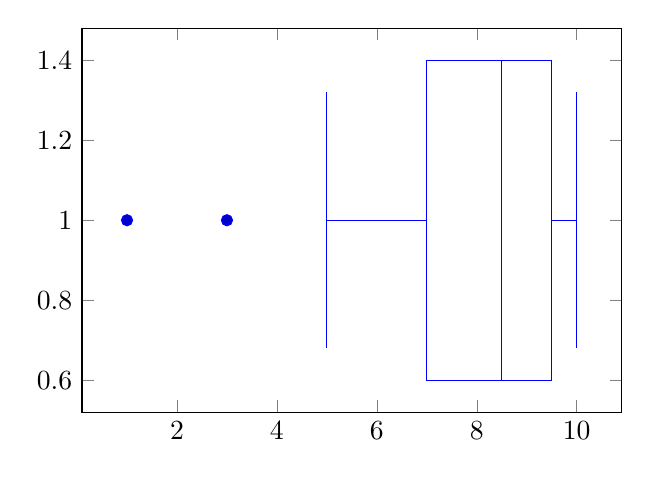
\begin{tikzpicture}
		\begin{axis}[
			y=2in,
			]
			\addplot+ [
			boxplot prepared={
				lower whisker=5,
				lower quartile=7,
				median=8.5,
				upper quartile=9.5,
				upper whisker=10,
			},
			]
			table [row sep=\\,y index=0] {
				data\\ 1\\ 3\\
			};
		\end{axis}
	\end{tikzpicture}
	\caption{Sample box plot, with outliers shown as scatters. The upper and lower whiskers show the data range, and the box shows the interquartile range.}
\end{figure}

\textbf{Chebyshev's inequality} : An inequality that measures the fraction of all data points that are a certain distance away from the sample mean. Given a dataset $ \{x_k\} $ with sample mean $ \bar{x} $ and standard deviation $ s $, the inequality gives a lower limit for the fraction of all data that is within $ [ \bar{x} - ks, \bar{x} + ks ] $ for $ k \geq 1$ and $ s > 0 $.

\begin{align}
	\frac{|S_{k}|}{n} \ \geq \ 1 - \frac{1}{k^{2}} 
\end{align}

For example, with $k = 2$, at least 75 \% of the data is within 2 standard deviations of the mean. The inequality is universal and this fraction may be much larger for tightly grouped datasets.

\textit{One-sided Chebyshev's inequality} : A stronger result can be used to find the fraction of data lying outside the interval  $ [ \bar{x} - ks, \bar{x} + ks ] $ with the above constraints on $ k, s $.

\begin{align}
	\frac{|N_{k}|}{n} \ \leq \ \frac{1}{1 + k^{2}} 
\end{align}

\textbf{Normally distributed datasets} : Most real-life datasets happen to be normally distributed. This is one of the most studied and extensively analysed probability distributions as a result. A normal distribution has approximately equal mean and median, and is not skewed left or right of its center.

For data obeying an approximately normal distribution, the fraction of all data points that lie within $ 1,\ 2 $ or $ 3 $ standard deviations from the mean is equal to 68\%, 95\%, and 99.7\% respectively.

Data sampled from a population that consists of subgroups that are not necessarily normally distributed ends up also not being normally distributed. Such data may be \textit{bimodal}, or \textit{multi-modal}, corresponding to two or more normal distributions being superposed to form a summed distribution.

\textbf{Correlation coefficient} : Two or higher dimensional datasets can be represented by an ordered set of data points $ \{x_i, y_i, ...\} $. The relationship between the individual dimensions is understood through the correlation $ r $. Commonly visualized using scatter plots.

Let a two dimensional data set have $ n $ data points $ \{x_i, y_i\} $. The mean and standard deviation for each dimension are $ \bar{x},\ \bar{y},\ s_x,\ s_y $ respectively. The sample correlation coefficient is defined as 

\begin{align}
	r \ =\ \frac{\sum\limits_{i = 1}^{n} (x_i - \bar{x}) (y_i - \bar{y})}{(n - 1) s_x s_y}
\end{align}

Some useful properties of $ r $ : 
\begin{align}
	-1 \leq r \leq 1
\end{align}
 
The extreme values are reached when the dimensions $ x $ and $ y $ are related by a straight-line equation $ y = a + bx $ depending on the sign of $ b $.

The value of $ r $ does not depend on the scale of the dimensions $ x $ or $ y $. This means that transforming $ \{x_i , y_i\} $ to $ \{a + b x_i , c + d y_i\} $ with $ bd > 0 $ will not change $ r $. This is equivalent to displacing or stretching the scatter plot along either of the axes.

The magnitude and sign or $ r $ respectively show the strength and the direction (positive or negative) of the correlation between the dimensions $ x $ and $ y $. Correlation does not imply causation. An underlying hidden variable is usually the cause for an observed correlation in all but the simplest of systems.

\textbf{Lorenz Curve} : This curve is meant to compare the contribution of the sum of the bottom $ j $ terms of a series to the sum of all terms of the series. Consider an ascending-sorted series of n entries $ \{x_i\} $. Using $ L(0) = 0 $ as a convention,  

\begin{align}
	L(j/n) = \frac{\text{sum of first $ j $ terms}}{\text{sum of all terms}}
\end{align}

\textbf{Gini Index} : Using the effect on the sample mean upon adding an additional large entry to a dataset, 

\begin{align}
	L(j/n) \leq j / n
\end{align}

A lorenz curve always lies to the bottom of the straight line with slope 1, unless all the entries in the dataset are equal. The deviation from this ideal condition is measured by relating the area under the Lorenz curve ($ B $), to the area under the reference line (1/2). The Gini Index ($ G $) is defined as

 \begin{align}
 	G = 1 - 2B
 \end{align}

\newpage


\chapter{Elements of Probability}


\begin{flushright}
	\textit{``You have to look at it from a Bayesian perspective."} 
\end{flushright}

\textbf{Interpretations of Probability} : A probability can be understood as either an inference based on many observations of similar events in the past, or as a quantitative estimate of the experimenter's belief in a hypothesis.

\textit{Frequentist} : Repeating the same experiment many times and observing the set of all outcomes enables one to assign a probability to a future outcome of that experiment as a property attached to the outcome itself. This probability is independent of the observer and is an inherent feature of the outcome and the underlying experiment.

\textit{Subjective / Bayesian} : This is a number indicating a person's belief in the outcome and is inherently subjective. Common in philosophy and economic theory.

\textbf{Sample Space} : set of all possible outcomes of an experiment (denoted by $ S $). An \textit{event} is a subset of the sample space containing one or more elements. It is commonly used to denote the outcome of an experiment.

The union of two events ($ E \cup F $) as well as their intersection ($ E \cap F $) are defined using the usual set theory norms. An intersection of two events with no common elements is the null event $ \varnothing $ (same notation as null set).

If $ E \cap F = \varnothing $, the events E and F are called \textit{mutually exclusive}.

From set theory, the complement of an event is the set of all elements in the sample space not contained in the event. $ E^{\complement}  = S - E$, making an event mutually exclusive with its complement. It follows that $ S^{\complement} = \varnothing $.

If one event contains all of the elements of another, then they are related by a subset-superset relationship. This is denoted by $ E \subset F $ or by $ F \supset E $. When two events are subsets of each other, they are considered identical or equal events.

\begin{align}
	\text{If} \qquad E \subset F \qquad \text{and} \qquad F \subset E \qquad \text{then, } \qquad E = F
\end{align}

Boolean algebra may be invoked to define the set operations on more than two events, as an extension of the above. The basic associative law, commutative law and distributive law of sets applies here to events trivially.

\textit{De-Morgan's Law} is a useful relation between the complements of unions or intersections of sets. 

\begin{align}
	(E \cup F)^{\complement} &= E^\complement \cap F^\complement \\
	%
	(E \cap F)^{\complement} &= E^\complement \cup F^\complement 
\end{align}

The above relations can be verified using \textit{Venn Diagrams}, which are the easiest way to graphically represent set algebra.

\textbf{Axioms of Probability} : For any experiment repeatedly conducted under identical conditions, the probability of an event will approach a fixed number asymptotically. This is the empirical probability ($ P $) of that event.

\begin{align}
	0 \leq P(E) \leq 1 \\
	%
	P(S) = 1 
\end{align}

For a set of mutually exclusive events $ \{ E_i \} $, 

\begin{align}
	P \left( \bigcup_{i = 1}^{n} E_i \right) &= \sum\limits_{i = 1}^{n} P(E_i) \\
	%
	P \left( \bigcap_{i = 1}^{n} E_i \right) &= 0
\end{align}

Using the fact that an event is mutually exclusive with its complement, 

\begin{align}
	P(E^\complement) = 1 - P(E)
\end{align}

\begin{figure}[H]
	\centering
	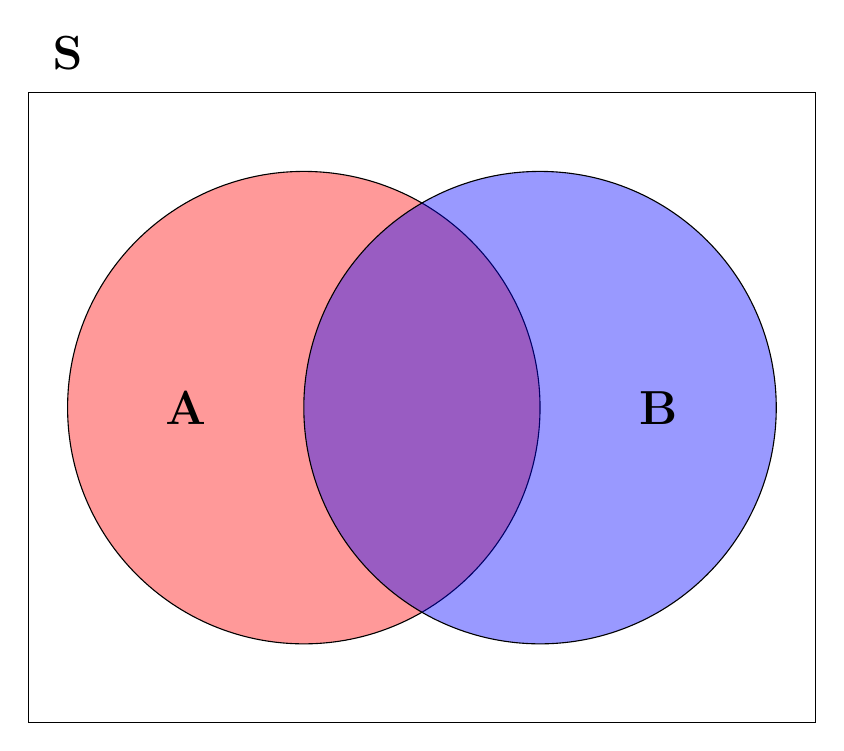
\begin{tikzpicture}
		%% You can adjust the opacity here. For venn diagrams it is convenient to have a low opacity so that you can see intersections
		\begin{scope} [fill opacity = .4]
			%% The draw command knows a lot of shapes. To make a rectangle you just need to specify two diagonal corners. Make sure you always have a semicolon at the end of your draw commands, otherwise latex flips out.
			\draw (-5,4) rectangle (5,-4);
			%% Similarly, you can make a circle by specifying the center and then the radius. You can also add a fill color, but if you're printing in black and white you'll probably want to remove that line.
			\draw[fill=red, draw = black] (-1.5,0) circle (3);
			\draw[fill=blue, draw = black] (1.5,0) circle (3);
			%% We can use the node command to label points. If you put your cursor on "LARGE" or "textbf" a box will drop down with size and text style options.
			\node at (-4.5,4.5) [text opacity = 1] {\LARGE\textbf{S}};
			\node at (-3,0) [text opacity = 1] {\LARGE\textbf{A}};
			\node at (3,0) [text opacity = 1] {\LARGE\textbf{B}};
		\end{scope}
		%% And now you have a venn diagram. Yay!
		%\draw[help lines](-5,5) grid (5,-6);    This line can draw the grid lines to help guide you. I use these when I'm writing the code and then delete this line when I publish the pdf.
	\end{tikzpicture}
	\caption{The purple area at the intersection of A and B is counted twice when naively adding the areas of A and B.} 
\end{figure} 

The probability of $ E \cup F $ is not the naive sum of the two individual probabilities, as seen in the Venn diagram here.

\begin{align}
	P(E \cup F) = P(E) + P(F) - P(E \cap F)
\end{align}

\textit{Odds} : the odds of an event is defined as a measure how much more likely an event is to occur compared to its complement. 

\begin{align}
	\frac{P(A)}{P(A^\complement)} = \frac{P(A)}{1 - P(A)}
\end{align}

\textbf{Equally likely outcomes} : It is common in real world experiments that every element of the sample space is equally likely. (Dice roll, coin flip, Lottery etc.). This special case simplifies the probability of an event to : 

\begin{align}
	P(E) = \frac{\text{number of element in E}}{\text{number of total elements}}
\end{align}

\textbf{Basic principles of counting} : For $ k $ repetitions of an experiment each with outcomes $ \{ n_1, n_2, ...., n_k \} $ respeectively, the total number of outcomes of the set of $ k $ repetitions is $ \left( \prod n_i  \right)$ 

\textit{Permutation} : The number of ways of selecting $ k $ out of $ n $ elements with sequence being relevant.

\begin{align}
	\Myperm{k} = \frac{n!}{(n-k)!} = \Mycomb{k} \ k! 
\end{align}

\textit{Combination} : The number of ways of selecting $ k $ out of $ n $ elements without regard to sequence. By convention, $ \Mycomb{0} = 1 $, using the fact that $ 0! = 1 $

\begin{align}
	\Mycomb{k} = \frac{n!}{(n-k)! \ k!} = \binom{n}{k}
\end{align}

\textbf{Conditional probability} : Useful when part of the outcome is known but not the full details. It looks at the probability of one event ($ A $) occurring, given another event ($ B $) has occurred. If the event $ B $ has occurred, then the sample space is now $ B $ instead of the initial $ S $. The desirable set of events now becomes the subset of elements in $ A $ that also happen to be in $ B $. This leads to the definition :

\begin{align}
	P(A|B) = \frac{P(A \cap B)}{P(B)}
\end{align}

Rearranging the above definition provides a convenient way to calculate the probability of the intersection of two events. 

\begin{align}
	P(A \cap B) = P(A|B)\ P(B)
\end{align}

\textbf{Bayes' theorem} : To find the probability of an event occurring, it is often useful to 'condition' it on the occurrence of another event. Using the definition of the complement of an event, 

\begin{align}
	P(A) &= P(A \cap B) + P(A \cap B^\complement) \\
	%
	P(A) &= P(A|B)\ P(B) + P(A|B^\complement)\ P(B^\complement)\\
	%
	P(A) &= P(B) \ P(A|B) + (1 - P(B))\ P(A|B^\complement)
\end{align}

Note that $ P(A) $ above becomes a linear interpolation between the two edges $ P(A|B) $ and $ P(A|B^\complement) $ with the sliding parameter being $ P(B) $. This is a useful perspective for many real-world problems.

An important pillar of Bayesian probability is the notion of updating a prior probability estimate after incorporating new (usually incomplete) information about the outcome.

The generalization of the conditional probability formula to more than two events is called Bayes' theorem. Let the set of mutually exclusive events $ \{ B_i \} $ be such that exactly one of them must occur.

\begin{align}
	\bigcup_{i = 1}^{n} B_i &= S \qquad \text{and} \qquad B_i \cap B_j = \varnothing \quad \forall \quad i \neq j \\
	%
	P(B_k|A) &= \frac{P(A \cap B_k)}{P(A)} = \frac{P(A | B_k) \ P(B_k)}{\sum_{i}P(A | B_i) \ P(B_i)}
\end{align}

The historical use of this formula was to update the probabilities of various hypotheses $ {B_i} $ after an experiment provides additional evidence $ A $.

\textbf{Independent events} : Two events are independent if the occurrence of one event does not affect the occurrence of the other event. 

\begin{align}
	P(A \cap B) &= P(A) \ P(B) \\
	%
	P(A|B) &= \frac{P(A \cap B)}{P(B)} = P(A)
\end{align}

If $ A $ and $ B $ are independent events, then so are $ A $ and $ B^\complement $. The above result extends to more than two events if any possible subset of the events is also independent. 

\newpage


\chapter{Random Variables and Expectation}


\begin{flushright}
	\textit{``Ch4 quote here"} \\
\end{flushright}

\textbf{Random Variables} : Some result of an experiment that the experimenter is interested in observing. This may not necessarily be the full details of the experiment. Ex : number of heads observed when tossing 10 coins, without worrying about the outcomes of the individual coin-tosses themselves. \\

Conventionally denoted by uppercase letters. A random variable can either be discrete or continuous. It is constrained by the same normalization condition as any other set of events making up a sample space. For the simple case of an integer valued random variable which ranges from $ \left[1, n\right] $\\

\begin{align}
	P(S) = P \left( \bigcup_{i = 1}^{n}\left\{X = i\right\} \right) = \sum_{1}^{n} P \left\{X = i\right\} = 1
\end{align} \\

\textit{Indicator random variable} : acts a Boolean flag indicating whether or not an event happens. Usually takes on two discrete values, 0 or 1. \\

\textbf{Cumulative distribution function} : For a continuous random variable, it is possible to define a function that measures the probability that this random variable $ (X) $ is lesser than or equal to some real value $ (x) $.\\

\begin{align}
	F(x) = P \left\{ X \leq x \right\}
\end{align} \\

Shorthand notation $ F ~ X $ is used to denote the fact that $ F $ is the distribution function for the random variable $ X $. Using the monotonically increasing nature of $ F $, for some real numbers $ b \geq a $

\begin{align}
	P \left\{ a < X \leq b \right\} = F(b) - F(a)
\end{align} \\

\textbf{Probability Mass function} : For a discrete random variable, this attempts to assign a probability to each of the distinct possible outcomes. There is an implicit assumption that the discrete values are mutually exclusive outcomes. Let the random variable $ X $ take on one of the possible values $ \left\{x_i\right\} $

\begin{align}
	p(a) &= P \left\{X = a\right\} \\
	%
	p(x) &\geq 0 \quad \forall \quad x \in \left\{x_i\right\} \\
	%
	p(x) &= 0 \quad \text{otherwise}
\end{align} \\

The equivalent normalization condition for the probability mass distribution is : 
\begin{align}
	\sum\limits_{i = 1} p(x_i) = 1
\end{align} \\

\textit{Discrete cumulative distribution function} : The equivalent of the above CDF for the special case of discrete random variables is : 

\begin{align}
	F(a) = \sum\limits_{x \leq a} p(x_i)
\end{align}

Notice that a discrete probability mass function looks like a bar plot while the corresponding CDF looks like a step function with the vertical step size being $ p(x_i) $ at every $ x = x_i $. \\

\textbf{Probability density function} : The analog of the PMF for a continuous random variable, using the fact that integration is the generalized version of summation. Consider a continuous random variable $ X $, and a set of real numbers $ B $.

\begin{align}
	P \left\{X \in B \right\} = \int\limits_{x \in B} f(x) \ \mathrm{d}x
\end{align}\\

The normalization condition on a PDF is that the area under the PDF curve over the entire real line sums to $ 1 $. : 

\begin{align}
	P \left\{X \in \left(-\infty , \infty \right) \right\} = \int\limits_{-\infty}^{\infty} f(x) \ \mathrm{d}x = 1
\end{align} \\

Even though the probability that a continuous random variable will assume a particular discrete value is zero, it does have a finite probability of assuming a value in a finite-sized continuous set. \\

\begin{align}
	P \left\{X = a \right\} &= 0 \\
	%
	P \left\{ a \leq X \leq b \right\} &= \int\limits_{a}^{b} f(x) \ \mathrm{d}x
\end{align}\\

The above relation can be used to infer that the probability of a random variable $ X $ having a value in an interval of size $ \epsilon $ around $ a $ is given by $ \epsilon f(a) $, assuming $ \epsilon $ is sufficiently small.  \\

For a random variable $ X $, a PDF (denoted $ f $) leads to a CDF (denoted $ F $) using the above integration. \\
\begin{align}
	F(a) &= P \left\{ X \in \left( -\infty, a \right]  \right\} = \int\limits_{-\infty}^{a} f(x) \ \mathrm{d}x \\
	%
	f(a) &= \frac{\mathrm{d}}{\mathrm{d}a} F(a)
\end{align} \\

\textbf{Jointly distributed RVs} : Extending the above definitions to more than one dimension in order to observe the relationship between two or more random variables, gives the joint CDF\\

\begin{align}
	F(x, y) = P \left\{ X \leq a, Y \leq b \right\}
\end{align} \\

Notice that dimensional reduction of this joint CDF, in order to isolate the CDF of just one of the random variables is achieved by integrating over all possible values of the other variables. \\

\begin{align}
	F_X (x) &= P \left\{ X \leq x \right\} \nonumber \\
	%
	&= P \left\{ X \leq x, Y < \infty \right\} \nonumber \\
	%
	&= F(x, \infty)
\end{align} \\

The joint PMF for two discrete variables $ X, Y $ each taking on values in the sets $ \left\{ x_i \right\}, \left\{ y_j \right\} $ is given by \\

\begin{align}
	p(x_i, y_j) = P \left\{ X = x_i, Y = y_j \right\}
\end{align}\\

Isolating the PMF of one of the variables simply involves summing over the probabilities of all possible values of the other variables. This is called the \textit{marginal PMF} of one of the many variables. A joint PMF can always be used to find the individual PMFs, but not vice versa.\\

\begin{align}
	P \left\{ X = x_i \right\} &= P \left( \bigcup_{j} \left\{ X = x_i, Y = y_j \right\} \right)  \nonumber\\
	%
	&= \sum\limits_{j} P \left\{ X = x_i, Y = y_j \right\} \nonumber\\
	%
	&= \sum\limits_{j} P \left\{x_i,y_j \right\}
\end{align} \\

\textit{Jointly continuous RVs} : Extending the definitions of a CDF and PDF to more than one dimension enables the definition of a joint probability. \\

Consider two continuous RVs $ X, Y $ whose domains are the real sets $ A, B $ respectively. The two-dimensional real set $ C = \left\{ (x,y) \ :\ x \in A, y \in B  \right\} $ consists of ordered pairs of real numbers.

\begin{align}
	P \left\{ (X, Y) \in C \right\} &= \iint\limits_{(x, y) \in C} f(x,y)\ \mathrm{d}x \  \mathrm{d}y \\
	%
	P \left\{ X \in A, Y \in B \right\} &= \int\limits_{B} \int\limits_{A} f(x,y)\ \mathrm{d}x \  \mathrm{d}y
\end{align} \\

The CDF of two jointly distributed continuous RVs using the prior one-dimensional case is\\

\begin{align}
	F(a, b) &= P \left\{ X \in \left( -\infty, a \right],  Y \in \left( -\infty, b \right] \right\} \nonumber \\
	%
	&= \int\limits_{-\infty}^{a} \int\limits_{-\infty}^{b} f(x,y)\ \mathrm{d}x \  \mathrm{d}y \\
	%
	f(a, b) &= \frac{\partial^2}{\partial a\  \partial b} F(a, b)
\end{align} \\

Integrating over an infinitesimal 2-D space, $ ( f(a, b)\ \mathrm{d}a \ \mathrm{d}b )$ is a representation of how likely the random vector $ (X, Y) $ is to be located in a $ \mathrm{d}a \ \mathrm{d}b $ vicinity of the point $ (a, b) $. \\

The marginal PDF of one of the two jointly distributed continuous variables is found by integrating over all possible values of the other variable.\\

\begin{align}
	P \left\{ X \in A \right\} &= P \left\{ X \in A, Y \in \left( -\infty, \infty \right) \right\} \nonumber \\
	%
	&= \int\limits_{A} \int\limits_{-\infty}^{\infty} f(x,y)\ \mathrm{d}y \  \mathrm{d}x \nonumber \\
	%
	&= \int\limits_{A} f_X (x)\ \mathrm{d}x
\end{align} \\

The above simplification uses the marginal PDF 

\begin{align}
	f_X (x) = \int\limits_{-\infty}^{\infty} f(x,y)\ \mathrm{d}y \\
	%
	f_Y (y) = \int\limits_{-\infty}^{\infty} f(x,y)\ \mathrm{d}x
\end{align} \\

\textbf{Independent Random Variables} : If for any two sets of real numbers $ A, B$, and events $ E_A, F_B $ defined by $ \left\{ X \in A \right\},  \left\{ Y \in B \right\}$,

\begin{align}
	P \left\{ X \in A, Y \in B \right\} &= P \left\{ X \in A \right\} \ P \left\{ Y \in B \right\} \\
	%
	P(E_A F_B) &= P(E_A)\ P(F_B) \nonumber
\end{align} \\

then, the RVs $ X, Y$ are independent.\\

A similar condition holds for the joint CDF $ F(a, b) $ of two independent RVs $ X, Y $

\begin{align}
	P \left\{ X \leq a, Y \leq b \right\} &= P \left\{ X \leq a \right\} \ P \left\{ Y \leq b \right\}  \nonumber \\
	%
	F(a, b) &= F_X(a)\ F_Y(b) \qquad \forall \qquad a, b
\end{align} \\

The condition for independence states that knowing the value of one RV does not change the distribution of another.The joint PMF of two independent discrete RVs also follows a similar constraint.

\begin{align}
	p(x, y) &= p_X(x)\ p_Y(y) \qquad \forall \qquad x, y
\end{align} \\

For continuous independent RVs, the correspoding constraint on their joint PDF is

\begin{align}
	f(x, y) &= f_X(x)\ f_Y(y) \qquad \forall \qquad x, y
\end{align} \\

For the generalized case of $ n $ independent RVs, the entire set of RVs is independent only if all possible subsets of these RVs are also independent. \\

\textbf{Conditional distributions} : Using the definition of conditional probability of two events, the conditional PMF for two RVs $ X, Y $ is defined as 

\begin{align}
	p_{X|Y}(x\ |\ y) &= P \left\{ X = x\ |\ Y = y \right\} \nonumber\\
	%
	&= \frac{P \left\{ X = x, Y = y \right\}}{P \left\{ Y = y \right\}} \nonumber\\
	%
	&= \frac{p(x, y)}{p_Y(y)}
\end{align} \\

The conditional PDF of two continuous RVs $ X, Y $ indicates the probability that $ X $ is in the vicinity of $ x $, given that $ Y $ is in the vicinity of $ y $. \\

\begin{align}
	f_{X|Y}(x\ |\ y) &= \frac{f(x, y)}{f_Y(y)} \\
	%
	P(X \in A\ |\ Y = y) &= \int\limits_{A} f_{X|Y}(x\ |\ y) \ \mathrm{d} x
\end{align}\\

\textbf{Expected value} : The expectation of a random variable $ X $, is simply the average value of that random variable weighted by the probabilities of each possible value. $ \mathbb{E}[X] $ need not be a value that $ X $ can actually take. It has the same units of measurement as $ X $ itself.\\

\begin{align}
	\mathbb{E}[X] = \sum\limits_{i} x_i\ P \left\{ X = x_i \right\} 
\end{align}\\

If $ I $ is an indicator RV for the event $ A $, then 

\begin{align}
	\mathbb{E}[I] = 1 \times P(A) + 0 \times P(A^\complement) = P(A)
\end{align}\\

\textit{Entropy} : A system of measuring the expected amount of information conveyed by a RV which can take on of $ n $ different values. This is measured in bits. \\

\begin{align}
	H(X) = -\sum\limits_{i = 1}^{n} p_i \ \log_{2}(p_i)
\end{align} \\

Here, the information conveyed by each possible value of the RV is summed using the probabilities as weights.

\begin{align}
	I\left\{X = x_i\right\} &= -\log_{2}(p_i) \\
	%
	H(X) &= \sum\limits_{i = 1}^{n} p_i \ I\left\{X = x_i\right\}
\end{align}\\

The expectation value of a continuous RV (analogous to the definition of the center of mass of a continuous object) is

\begin{align}
	\mathbb{E}[X] = \int_{-\infty}^{\infty} x\ f(x)\ \mathrm{d}x
\end{align} \\

\textbf{Properties of expected value} : With a known PDF for a random variable $ X $, there are two approaches to finding the expected value of some function of $ X $. \\

$ \mathbb{E}[G(X)] = \mathbb{E}[Y] $ uses the substitution $ Y = G(X) $ to find the values taken by this new RV $ Y $ and then apply the weighted sum method. \\

For the less trivial case of a continuous RV $ X $, an existing PDF $ f_X (x) $ can be used to find the CDF $ F_Y(a) $ and then differentiated to produce the new PDF $ f_Y(a) $. The integral formula for $ \mathbb{E}[Y] $ is then easily applied. A more straightforward method is as follows, 

\begin{align}
	\mathbb{E}[g(X)] &= \sum\limits_{x} g(x)\ p(x)  \qquad \text{for discrete RV} \\
	%
	\mathbb{E}[g(X)] &= \int\limits_{x} g(x)\ f(x)\ \mathrm{d}x  \qquad \text{for continuous RV} \\
	%
	\mathbb{E}[aX + b] &= a \mathbb{E}[X] + b \nonumber
\end{align}\\

\textbf{Moments} : The expectation value generalized to higher powers is defined as the moment. The special case of $ n = 1 $ is merely the expected value. \\

\begin{align}
	\mathbb{E}[X^n] &= \sum_{x} x^n\ p(x) \qquad \text{for discrete RV} \\
	%
	\mathbb{E}[X^n] &= \int_{-\infty}^{\infty} x^n\ f(x)\ \mathrm{d}x \qquad \text{for continuous RV}
\end{align} \\

Generalizing to more than two RVs $ X, Y $ along with a function $ g(x,y) $ of two variables,

\begin{align}
	\mathbb{E}[g(X, Y)] &= \sum\limits_{x} \sum\limits_{y} g(x, y)\ p(x, y)  \qquad \text{for discrete RV} \\
	%
	\mathbb{E}[g(X, Y)] &= \int\limits_{-\infty}^{\infty} \int\limits_{-\infty}^{\infty} g(x, y)\ f(x, y)\ \mathrm{d}x \ \mathrm{d}y  \qquad \text{for continuous RV} \\
	%
	\mathbb{E}[X + Y] &= \mathbb{E}[X] + \mathbb{E}[Y] \nonumber
\end{align} \\

\textit{Mean value as an RV predictor} : Let the RV $ X $ with mean $ \mu $ be predicted to have a value $ c $ by an experimenter. From the point of view of minimizing the average squared error, the best prediction of the RV outcome is its mean.\\

\begin{align}
	\mathbb{E}[(X - c)^2] &= \mathbb{E}[(X - \mu)^2] + (\mu - c)^2 \nonumber \\
	%
	&\geq \mathbb{E}[(X - \mu)^2] 
\end{align} \\

\textbf{Variance} : The conventional measure of the spread in the values of a random variable, denoted by $ \mathrm{Var}(X) $. This is used alongside the expected value $ \mathbb{E}[X] $ to summarize the RV. \\

\begin{align}
	\mathrm{Var}(X) &= \mathbb{E}[(X - \mu)^2] \\
	%
	\mathrm{Var}(X) &= \mathbb{E}[X^2] - (\mathbb{E}[X])^2
\end{align} \\

For an indicator RV $ I $, which is a binary $ \left\{0, 1\right\} $ switch indicating the occurrence of event $ A $, the variance is 

\begin{align}
	\mathrm{Var}(I) &= P(A) [1 - P(A)]
\end{align} \\

The variance transforms using the following relation upon change of RV, 
\begin{align}
	\mathrm{Var}(aX + b) &= a^2 \ \mathrm{Var}(X) \\
	%
	\mathrm{Var}(b) &= 0 \\
	%
	\mathrm{Var}(X + b) &= \mathrm{Var}(X)
\end{align} \\

\textit{Standard Deviation} : defined as the square root of the variance, measured in the same units as the underlying RV. 
\begin{align}
	s_X = \sqrt{\mathrm{Var}(X)}
\end{align} \\

\textbf{Covariance} : $ \mathrm{Var}(X + Y) \neq \mathrm{Var}(X) + \mathrm{Var}(Y) $ except for the special case of $ X, Y $ being independent RVs. Consider the two RVs $ X, Y $ with means $ \mu_x , \mu_y$ respectively. \\

\begin{align}
	\mathrm{Cov}(X, Y) &= \mathbb{E}[(X - \mu_x)(Y - \mu_y)] \\
	%
	\mathrm{Cov}(X, Y) &= \mathbb{E}[XY] - \mathbb{E}[X] \ \mathbb{E}[Y]
\end{align} \\

Covariance has the following useful properties, 

\begin{align}
	\mathrm{Cov}(X, Y) &= \mathrm{Cov}(Y, X) \\
	%
	\mathrm{Cov}(X, X) &= \mathrm{Var}(X) \\
	%
	\mathrm{Cov}(aX, Y) &= a \ \mathrm{Cov}(X, Y) \\
	%
	\mathrm{Cov}(X_1 + X_2, Y) &= \mathrm{Cov}(X_1, Y) + \mathrm{Cov}(X_2, Y)
\end{align} \\

Generalizing the above relation to two sets of RVs $ \left\{X_i\right\}, \left\{Y_j\right\} $ gives the following relation, 
\begin{align}
	\mathrm{Cov} \left( \sum\limits_{i}X_i , \sum\limits_{j}Y_j \right) = \sum\limits_{i} \sum\limits_{j} \mathrm{Cov} (X_i, Y_j)
\end{align} \\

Replacing the $ \left\{Y_j\right\} $ set of RVs with another copy of the first set $  \left\{X_i\right\} $ in the above relation, gives a formula for the variance of the sum of RVs. \\

\begin{align}
	\mathrm{Var} \left( \sum\limits_{i}X_i \right) = \sum\limits_{i} \mathrm{Var}(X_i) + \sum\limits_{i} \sum\limits_{j \neq i} \mathrm{Cov} (X_i, X_j)
\end{align} \\

For the special case of independent RVs $ X, Y $, and thus for a set of independent RVs $ \left\{X_i\right\} $

\begin{align}
	\mathrm{Cov}(X, Y) &= 0 \\
	%
	\mathrm{Var} \left( \sum\limits_{i}X_i \right) &= \sum\limits_{i}\mathrm{Var}(X_i) 
\end{align} \\

\textbf{Correlation} : Normalizing the covariance of two RVs by the product of their standard deviations results in a quantity $ \mathrm{Corr}(X, Y) $ which lies in the range $ \left[-1, 1\right] $. A positive correlation shows that an increase in $ X $ tends to be accompanied by an increase in $ Y $ and vice versa. \\

\begin{align}
	\mathrm{Corr}(X, Y) = \frac{\mathrm{Cov}(X, Y)}{s_x s_y}
\end{align} \\

Consider two indicator RVs $ X, Y $ for two underlying events $ A, B $. Now, the correlation measures the increase in probability of occurrence of $ A $ given the occurrence of $ B $. 

\begin{align}
	\mathrm{Corr}(X, Y) &> 0  \qquad \Leftrightarrow \qquad P \left\{ Y = 1\ |\ X = 1 \right\} > P \left\{ Y = 1 \right\}
\end{align} \\

\textbf{Moment generating functions} : A function which gives all of the moments of a RV $ X $, upon repeated differentiation. This is defined for all values of the parameter $ t $.\\

\begin{align}
	\phi(t) &= \mathbb{E}[e^{tX}] \\
	%
	\phi(t) &= \sum_{x} e^{tx} \ p(x) \qquad \text{for discrete RV} \\
	%
	\phi(t) &= \int_{-\infty}^{\infty} e^{tx}\ f(x)\ \mathrm{d}x \qquad \text{for continuous RV} 
\end{align} \\

Some useful properties of the function $ \phi(t) $ when evaluated at $ t = 0 $,

\begin{align}
	\phi^n (0) &= \mathbb{E}[X^n] \qquad n \geq 1 \\
	%
	\phi'(0) &= \mathbb{E}[X] \qquad \text{is the mean} \\
	%
	\phi''(0) - \left(\phi'(0)\right)^2 &= \mathrm{Var}(X) \qquad \text{is the variance}
\end{align} \\

The moment generating function corresponds one-to-one with the distribution function of a given RV. Also, for the special case of two independent RVs $ X, Y $

\begin{align}
	\phi_{X + Y}(t) = 	\phi_{X}(t)\ \phi_{X}(t)
\end{align} \\

\textbf{Markov's inequality} : For a random variable $ X $, that only takes non-negative values, and some $ a > 0 $,\\
\begin{align}
	P\left\{ X \geq a \right\} \leq \frac{\mathbb{E}[X]}{a}
\end{align} \\

\textbf{Chebyshev's inequality} : Using $ a = k^2 $ and the non-negative RV $\left| X - \mu \right|$,\\
\begin{align}
	P\left\{( X - \mu)^2 \geq k^2 \right\} &\leq \frac{\mathbb{E}[(X - \mu)^2]}{k^2} \nonumber \\
	%
	P\left\{\left| X - \mu \right| \geq k\right\} &\leq \frac{\sigma^2}{k^2} \nonumber \\
	%
	P\left\{\left| X - \mu \right| \geq n\sigma \right\} &\leq \frac{1}{n^2}
\end{align} \\

The above inequalities help derive bounds on probabilities when only the mean and/or variance of the distribution is known. \\

\textbf{Weak Law of large numbers} : Consider a set of independent, identically distributed random variables $ \left\{X_i\right\} $, each with the same mean. $ \mathbb{E}[X_i] = \mu $, and $ \epsilon > 0 $.\\

\begin{align}
	P \left\{ \left| \frac{ X_1 + X_2 + \dots + X_n }{n} - \mu \right|\  >\ \epsilon \right\} \to 0 \qquad
	\text{as } x \to \infty
\end{align} \\

The mean of the first $ n $ experimental outcomes measuring the RV $ X $ is a distance $ \epsilon $ away from the true expected value $ \mu $. This distance approaches $ 0 $ as $ n $ approaches $ \infty $.\\

A restatement of the above uses the experiment of sampling a fixed distribution $ n $ times and measuring the distance between the sample mean and the true mean. As the number of samples increases, the sample mean approaches the true mean asymptotically.
\newpage
\chapter{Special Random Variables}


\begin{flushright}
	\textit{``Wow, this cumulative distribution function has a closed form expression!"} 
\end{flushright}

\textbf{Bernoulli RV} : Consider an experiment that only has two outcomes - success and failure. This can be represented by a RV that takes values $ \left\{0, 1\right\} $, with PMF

\begin{align}
	P \left\{X = 0\right\} &= 1-p \nonumber \\
	%
	P \left\{X = 1\right\} &= p \qquad \text{with} \qquad p \in [0, 1] \\
	%
	\mathbb{E}[X] &= p \\
	%
	\mathrm{Var}(X) &= p(1-p)
\end{align}

\textbf{Binomial RV} : Consider a set of $ n $ independent Bernoulli RVs. The total number of successes is called a Binomial RV, because of the PMF resembling binomial coefficients. This automatically makes the PMF defined only at non-negative integer values.

\begin{figure}[!h]
	\centering
	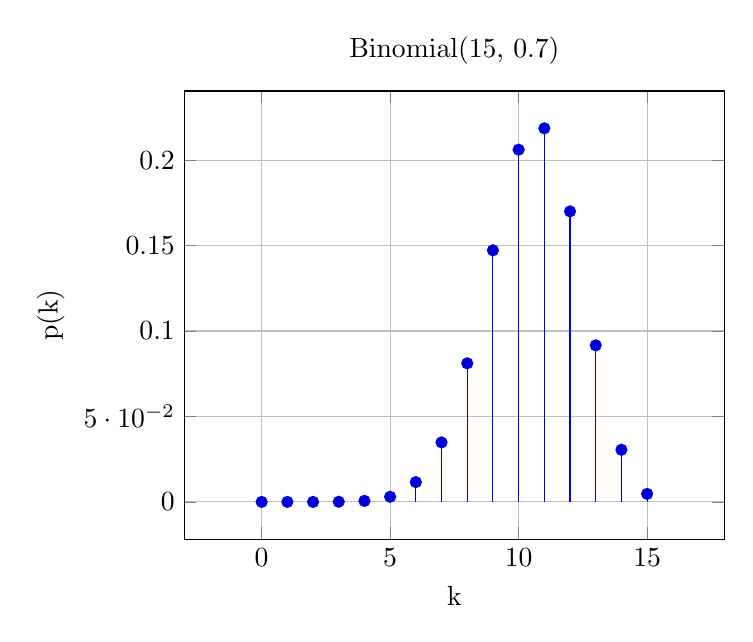
\begin{tikzpicture}
		\begin{axis}[enlarge x limits=0.2, grid = both,
			xlabel = k, ylabel = p(k), title = {Binomial(15, 0.7)}]
			\addplot+[ycomb] plot coordinates {( 0 , 0.0 ) ( 1 , 0.0 ) ( 2 , 0.0 ) ( 3 , 0.0001 ) ( 4 , 0.0006 ) ( 5 , 0.003 ) ( 6 , 0.0116 ) ( 7 , 0.0348 ) ( 8 , 0.0811 ) ( 9 , 0.1472 ) ( 10 , 0.2061 ) ( 11 , 0.2186 ) ( 12 , 0.17 ) ( 13 , 0.0916 ) ( 14 , 0.0305 ) ( 15 , 0.0047 ) };  
		\end{axis} 
	\end{tikzpicture}
\end{figure}


The two defining parameters of a Binomial RV are $ (n, p) $ where $ n $ is the number of trials and $ p $, the probability of each trial being independently a success.

\begin{align}
	P \left\{X = i\right\} &= \binom{n}{i}\ p^i \ (1-p)^{n-i}
\end{align}

Proving the normalization constraint requires the binomial theorem,
\begin{align}
	[p + (1-p)]^n &= 1^n = 1 \nonumber \\
	%
	\sum\limits_{i=0}^{n} P \left\{X = i\right\} &= \sum\limits_{i=0}^{n} \binom{n}{i}\ p^i \ (1-p)^{n-i}  = 1
\end{align}

Using the fact that the $ \mathbb{E}[\sum X] $ when the RVs are independent, reduces to $ \sum \mathbb{E}[X] $, and a similar rule for the variance,

\begin{align}
	\mathbb{E}[X] &= np \\
	%
	\mathrm{Var}(X) &= np(1-p)
\end{align}

If $ X_1, X_2 $ are two binomial RVs with parameters $ (n_1, p) $ and $ (n_2, p) $, then the RV $ X = X_1 + X_2 $ is also a binomial RV with parameters $ (n_1 + n_2, p) $ 

\textbf{Poisson RV} : Consider an RV that takes on non-negative integer values along with a parameter $ \lambda > 0 $, whose PMF is given by


\begin{align}
	P \left\{X = i\right\} &= e^{-\lambda}\ \frac{\lambda^i}{i!}
\end{align}

Using the Taylor series expansion of the exponential function, the normalization constraint is proved as follows,


\begin{align}
	e^x &= 0 + 1 + \frac{x^2}{2!} + \frac{x^3}{3!} + \dots \nonumber \\
	%
	\sum\limits_{i=0}^{\infty} P \left\{X = i\right\} &= e^{-\lambda} \left(\sum\limits_{i=0}^{\infty} \frac{\lambda^i}{i!}\right) = e^{-\lambda} \ e^{\lambda} = 1
\end{align}

\begin{figure}[!h]
	\centering
	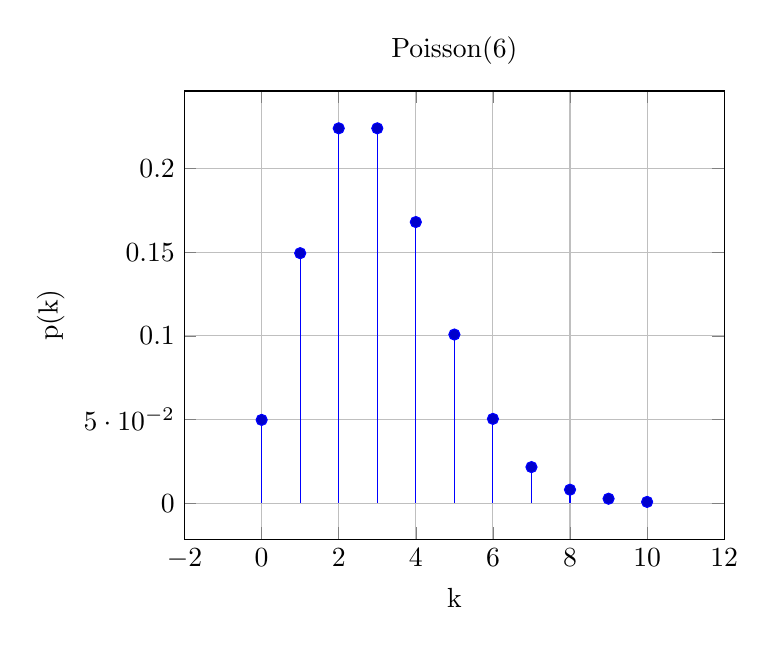
\begin{tikzpicture}
		\begin{axis}[enlarge x limits=0.2, grid = both,
			xlabel = k, ylabel = p(k), title = {Poisson(6)}]
			\addplot+[ycomb] plot coordinates {( 0 , 0.0498 ) ( 1 , 0.1494 ) ( 2 , 0.224 ) ( 3 , 0.224 ) ( 4 , 0.168 ) ( 5 , 0.1008 ) ( 6 , 0.0504 ) ( 7 , 0.0216 ) ( 8 , 0.0081 ) ( 9 , 0.0027 ) ( 10 , 0.0008 ) };  
		\end{axis} 
	\end{tikzpicture}
\end{figure}

Using the derivatives of the moment-generating function $ \phi(t) $, gives the mean and variance,

\begin{align}
	\phi(t) &= \mathbb{E}[e^{tX}] = \exp\left\{\lambda (e^t - 1)\right\}\\
	%
	\mathbb{E}[X] &= \lambda \\
	%
	\mathrm{Var}(X) &= \lambda
\end{align}

In the limit of $ n $ very large and $ p $ very small for a binomial RV with parameters $ (n, p) $, it can be approximated using a Poisson RV with parameter $ \lambda = np $.

\begin{align}
	P \left\{X = i\right\}\ =\ \binom{n}{i}\ p^i\ (1-p)^{n-i}\ \approxeq\ e^{-np}\ \frac{(np)^i}{i!}
\end{align}

An evern more general result, uses $ n $ independent trials each with probability of success $ p_i \ \forall\ i \in \left\{1, \dots, n\right\}$, with the condition that $ n $ is large and all of the $ p_i $ are small. The Poisson RV approximation can then me made with parameter $ \lambda = \sum p_i $.

Weak independence is measured by the conditional probability of one event succeeding given another has already succeeded. If these two values are approximately equal, then this approximation applies.

If $ X_1, X_2 $ are independently Poisson distributed with parameters $ \lambda_1, \lambda_2 $, then their sum $ X = X_1 + X_2 $ is also Poisson distributed with parameter $ \lambda_1 + \lambda_2 $. Since the moment generating function of a distribution uniquely determines it,

\begin{align}
	\phi (t) &= \mathbb{E}[e^{tX}] = \mathbb{E}[e^{t(X_1 + X_2)}] \nonumber \\
	%
	&= \mathbb{E}[e^{tX_1}] \mathbb{E}[e^{tX_2}] \nonumber \\
	%
	&= \exp\left\{(\lambda_1 + \lambda_2) (e^t - 1)\right\}
\end{align}

As an extension of the above, consider a total of $ N $ events, of which $ N_1, N_2 $ represent the number of events of types 1 and 2, with probabilities $ p $ and $ 1-p $ respectively. Also, $ N = N_1 + N_2 $.

If $ N $ is Poisson distributed with mean $\lambda$, then $ N_1, N_2 $ are also Poisson distributed with mean $ p\lambda $ and $ (1-p)\ \lambda $ respectively. This easily extends to more than two possible event types.

\begin{align}
	P\left\{N = n+m\right\} &= e^{-\lambda} \ \frac{\lambda^{n+m}}{(n+m)!} \nonumber \\
	%
	P\left\{N_1 = n\right\} &= e^{-p\lambda} \ \frac{(p\lambda)^{n}}{(n)!} \nonumber \\
	%
	P\left\{N_2 = m\right\} &= e^{-(1-p)\lambda} \ \frac{((1-p)\lambda)^{m}}{(m)!}
\end{align}

\textbf{Hypergeometric RV} : Consider a set of $ N+M $ objects of which $ N $ are acceptable and $ M $ defective. Let an experiment involve choosing $ n $ random objects out of $ N+M $, and then measure the number of acceptable objects picked using the RV $ X $.

$ X \in \left\{0, 1, \dots, \min(n, N) \right\} $, as the number of acceptable objects picked cannot exceed $ N $. This is a hypergeometric RV with PMF given by,

\begin{align}
	P \left\{X = i\right\} &= \ddfrac{\binom{N}{i}\ \binom{M}{n-i}}{\binom{N+M}{n}}
\end{align}

The parameters are $ (N, M, n) $, with the RV taking on non-negative integer values. If the proportion of acceptable objects is $ p $, then,

\begin{align}
	\mathbb{E}[X] &= \frac{nN}{N+M} = np \\
	%
	\mathrm{Var}(X) &= \frac{nNM}{(N+M)^2}\ \left(1 - \frac{n-1}{N+M-1}\right) \nonumber \\
	%
	&=  np\ (1-p)\ \left(1 - \frac{n-1}{N+M-1}\right)
\end{align}

Notice from the variance that the hypergeometric distribution converges to a binomial distribution in the limit $ N+M \to \infty $ and thus $ n \lll N $.

Consider two binomial RVs $ X, Y $ with parameters $ (n, p) $ and $ (m, p) $ respectively. The PMF of $ X $, given $ X+Y = k $ is given by,

\begin{align}
	P \left\{X = i\ |\ X+Y = k\right\} &= \ddfrac{\binom{n}{i}\ \binom{m}{k-i}}{\binom{n+m}{k}}
\end{align}

The denominator uses the fact that $ X+Y $ is also binomial with paramters $ (n+m, p) $, and the expression measures the probability that $ i $ out of the $ k $ successes were contributed by the RV $ X $.

This turns out to be a hypergeomtric RV measuring how many out of $ k $ objects picked were of type $ X $.


\textbf{Uniform RV} : Consider a continuous RV over the closed interval $ \left[\alpha, \beta\right] $, with PDF given by

\begin{align}
	f(x) &= \frac{1}{\beta - \alpha} & \text{if}\ x \in \left[\alpha, \beta\right] \\
	%
	f(x) &= 0 & \text{otherwise} \nonumber
\end{align}

The normalization constriant is easily proven using the Riemann integration of a continuous function.

\begin{align}
	P \left\{a < X < b\right\} &= \int\limits_{a}^{b} f(x)\ \mathrm{d} x = \frac{b - a}{\beta - \alpha} \\
	%
	P \left\{-\infty < X < \infty\right\} &= \int\limits_{-\infty}^{\infty} f(x)\ \mathrm{d} x = 1 \nonumber
\end{align}

Using simple polynomial integrations,

\begin{align}
	\mathbb{E}[X] &= \frac{\alpha + \beta}{2} \\
	%
	\mathrm{Var}(X) &= \frac{(\beta - \alpha)^2}{12} 
\end{align}


By computer science convention, a \textit{random number} is a uniformly distributed real number in the range $ [0, 1] $. A simple linear transformation $ Y = aX + b $ can be used to rescale this random number to the domain $ [b, a+b] $.

An important application of uniform RV sampling is Monte Carlo simulations, often used to estimate a parameter by performing a large number of experiments and using a frequentist approach to assign probabilities.

\textbf{Normal RV} : The most consistent distribution underlying real-world datasets, and as a result the most well-studied. This was originally introduced as an approximation to binomial distributions with extremely large $ n $. Using the mean and variance as parameters, the PDF for $ X \sim \mathcal{N}(\mu, \sigma^2) $ is defined as

\begin{align}
	f(x) = \frac{1}{\sqrt{2 \pi \sigma^2}} \exp \left[\frac{- (x - \mu)^2}{2\sigma^2}\right] \qquad \forall \quad x \in \mathbb{R}
\end{align}

This distribution is also called a bell curve. It is symmetric about $ \mu $, which is also its maximum.

\begin{align}
	\mathbb{E}[X] &= \mu \\
	%
	\mathrm{Var}(X) &= \sigma^2 \\
	%
	\mathbb{E}[aX + b] &= a\ \mu + b \nonumber \\
	%
	\mathrm{Var}(aX + b) &= a^2 \ \sigma^2 \nonumber 
\end{align}

\textit{Standard normal RV} : A normal RV with mean 0 and variance 1. Any normal RV $ X $ can be converted into a standard normal RV ($ \Phi $), using the transform $ Z = (X - \mu) / \sigma$

\begin{align}
	X &\sim \mathcal{N}(\mu, \sigma^2) \nonumber \\
	%
	Z &\sim \mathcal{N}(0, 1) \qquad \text{using} \qquad Z = \frac{X - \mu}{\sigma}
\end{align}

\begin{figure}[H]
	\centering
	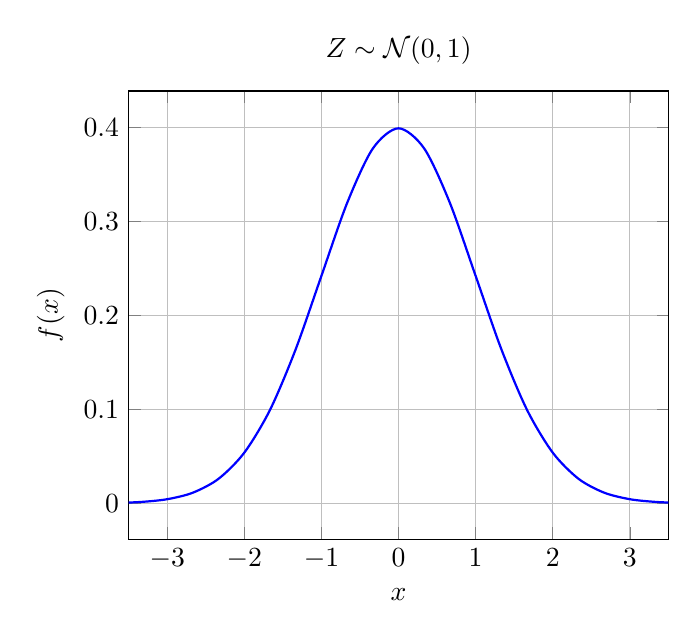
\begin{tikzpicture}
		\begin{axis}[xlabel=$x$, grid = both, xmin = -3.5, xmax = 3.5, ylabel = {$f(x)$}, title = {$ Z \sim \mathcal{N}(0, 1) $}]
			\addplot[thick, smooth, draw=blue][name path = f2, domain = -4:4]{(1/sqrt(2*pi)*exp(-x*x*0.5))};
		\end{axis}
	\end{tikzpicture}
\end{figure}

The numerical value of the standard normal RV $ (\Phi) $ has historically been computed using approximations and the CDF tabulated to a high degree of precision. Such a reference table is used to actually assign probabilities to $ \Phi $ 

\begin{align}
	\Phi(x) &= \int\limits_{-\infty}^{x} \frac{1}{\sqrt{2 \pi}} \exp \left(\frac{-y^2}{2}\right)\ \mathrm{d}y \\
	%
	P\left\{X < b\right\} &= P \left\{\frac{X - \mu}{\sigma} < \frac{b - \mu}{\sigma}\right\} = \Phi \left\{\frac{b - \mu}{\sigma}\right\} \\
	%
	\Phi(-x) &= 1 - \Phi(x)
\end{align}

The moment generating function of a normal RV uses the result for a standard normal RV.

\begin{align}
	\phi_Z (t) &= \mathbb{E}[e^{tZ}] = \exp\left(\frac{t^2}{2}\right)	  \\
	%
	\phi_X (t) &= \mathbb{E}[e^{t\mu}\ e^{t \sigma Z}] = \exp\left(\mu t + \frac{\sigma^2 t^2}{2}\right)
\end{align}

This also leads to the fact that the sum of independent normal RVs is also a normal RV. Consider a set of normal RVs $ \left\{X_i\right\} $ with mean and variance $ \left\{\mu_i\right\},\ \left\{\sigma^2_i\right\} $ respectively. From the moment-generating function,

\begin{align}
	\mathbb{E}[e^{tX}] &= \prod_{i=1}^{n} \mathbb{E}[e^{tX_i}] \nonumber \\
	%
	\mu &= \sum\limits_{i=1}^{n} \mu_i \qquad \text{and} \qquad \sigma^2 = \sum\limits_{i=1}^{n} \sigma_i^2
\end{align}

\textit{Percentile and z-score} : By convention, $ \alpha $ and $ z_\alpha $ are called the \textit{p-value} and \textit{z-score} respectively. The $ 100 \alpha $ percentile of a standard normal RV is that value $ x = z_\alpha $ for which,

\begin{align}
	P \left\{Z > z_\alpha\right\} &= 1 - \Phi(z_\alpha) = \alpha
\end{align}

\begin{figure}[H]
	\centering
	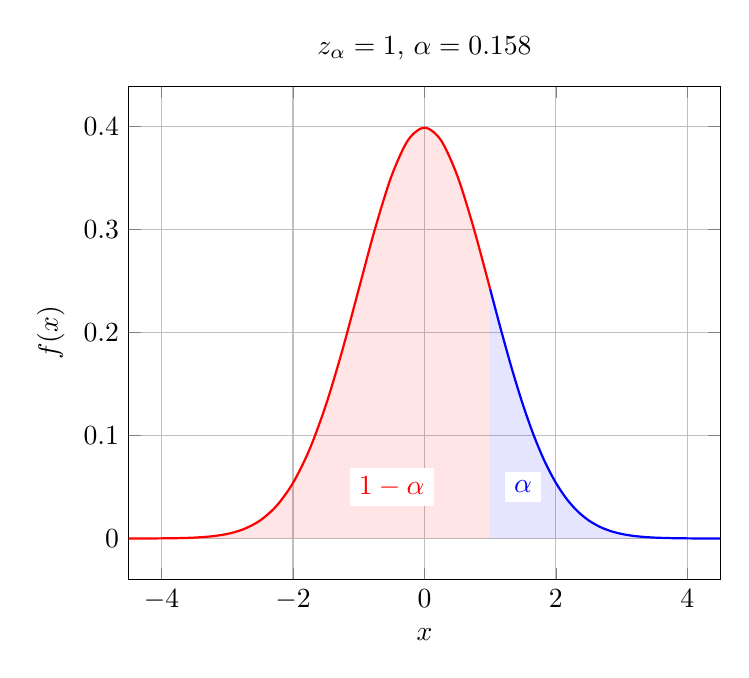
\begin{tikzpicture}
		\begin{axis}[width = 0.75\textwidth,xlabel=$x$, ylabel=$ f(x) $, grid = both, xmin = -4.5, xmax = 4.5, title = {$z_\alpha = 1$, $ \alpha = 0.158 $}]
			\addplot[thick, smooth, draw=red][name path = f1, domain = -5:1]{(1/sqrt(2*pi)*exp(-x*x*0.5))};
			\addplot[thick, smooth, draw=blue][name path = f2, domain = 1:5]{(1/sqrt(2*pi)*exp(-x*x*0.5))};
			
			\path[name path=axis1] (axis cs:-5,0) -- (axis cs:1,0);
			\path[name path=axis2] (axis cs:1,0) -- (axis cs:5,0);
			
			\addplot [thick,color=red,fill=red, fill opacity=0.1] fill between[of=f1 and axis1,];
			\addplot [thick,color=red,fill=blue, fill opacity=0.1] fill between[of=f2 and axis2,];
			
			\node[color=blue, fill=white] at (axis cs: 1.5,.05) {$ \alpha $};
			\node[color=red, fill=white] at (axis cs: -0.5,.05) {$ 1 - \alpha $};
			
		\end{axis}
	\end{tikzpicture}
\end{figure}


\textbf{Exponential RV} :  Consider a continuous RV defined over the real line with PDF and CDF given by

\begin{align}
	f(x) &= \lambda\ e^{-\lambda x} & \text{if}\ x \in \left[0, \infty\right) \\
	%
	f(x) &= 0 & \text{otherwise} \nonumber
\end{align}


\begin{figure}[H]
	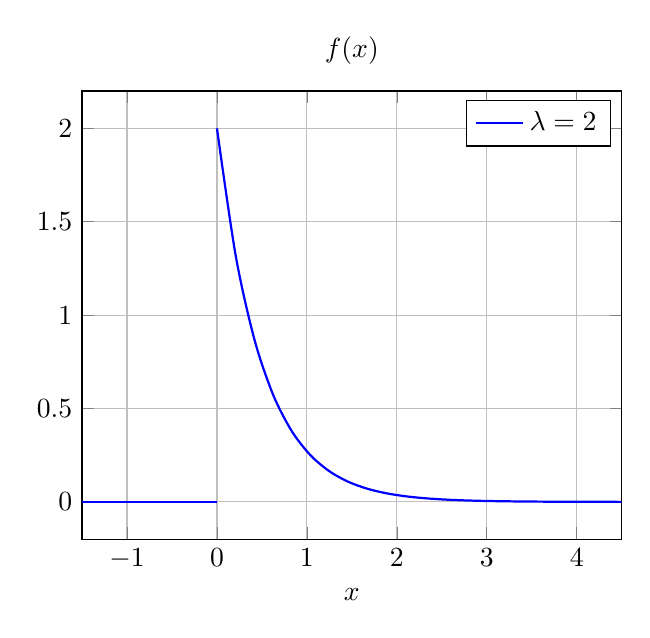
\begin{tikzpicture}
		\begin{axis}[xlabel=$x$, grid = both, xmin = -1.5, xmax = 4.5, title = {$f(x)$}]
			\addplot[thick, smooth, draw=blue][name path = f1, domain = -2:0]{0};
			\addplot[thick, smooth, draw=blue][name path = f1, domain = 0:5]{2*exp(-2*x)};
			\addlegendentry{$ \lambda = 2$}
		\end{axis}
	\end{tikzpicture}
	%
	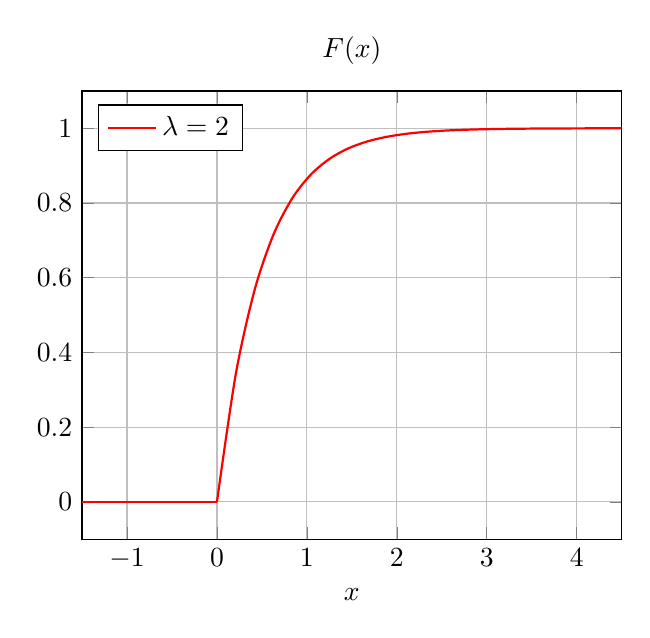
\begin{tikzpicture}
		\begin{axis}[xlabel=$x$, grid = both, xmin = -1.5, xmax = 4.5, title = {$F(x)$}, legend pos = north west]
			\addplot[thick, smooth, draw=red][name path = f1, domain = -2:0]{0};
			\addplot[thick, smooth, draw=red][name path = f1, domain = 0:5]{1 - exp(-2*x)};
			\addlegendentry{$ \lambda = 2$}
		\end{axis}
	\end{tikzpicture}
\end{figure}


The parameter $ \lambda $ , called the \textit{rate}, solely defines the exponential RV with a CDF,

\begin{align}
	F(x) &= 1 - e^{-\lambda x} \qquad \forall \ x \geq 0
\end{align}

The exponential distribution if observed most commonly as the distribution of time intervals between successive occurrences of natural events. The moment-generating function gives the mean and variance as follows

\begin{align}
	\phi(t) &= \frac{\lambda}{\lambda - t} \qquad \forall\ t < \lambda \\
	%
	\mathbb{E}[X] &= \frac{1}{\lambda} \\
	%
	\mathrm{Var}(X) &= \frac{1}{\lambda^2}
\end{align}

An important property exclusive to the exponential function is that it is \textit{memoryless}, or \textit{self-similar} across time. This is mathematically represented as

\begin{align}
	P \left\{X > t+s\ |\ X > t \right\} &= P \left\{X > s \right\} \qquad \forall \ s, t\geq 0
\end{align}

The probability of an item functioning for $ s $ additional time does not depend on the fact that it has functioned for $ t $ time already.

The minimum of a set of independent exponential RVs $ \left\{X_i\right\} $ with parameters $ \left\{\lambda_i\right\} $ is also an exponential RV. This is easily understood as the lifetime of a system with many components all of which are necessary for it to function.

\begin{align}
	P \left\{\mathrm{min}(X_1, X_2, \dots, X_n) > x\right\} &= e^{-\lambda x} \nonumber \\
	%
	\lambda &= \sum_{i=1}^{n} \lambda_i
\end{align}

An independent exponential RV transforming as $ X \to cX $ causes the rate to change as $ \lambda \to \lambda/c $.

\textbf{Poisson process} : Consider a process where events happen randomly such that $ N(t) $ denotes the number of events in the time $ [0, t] $. This is a Poisson process with \textit{rate} $ \lambda $, if

\begin{itemize}
	\item $ N(0) = 0 $, with $ t = 0 $ denoting the start of the process.
	
	\item Disjoint time intervals have an independent number of events occurring in them.
	
	\item The number of events in a given interval has a distribution depending only on the length of the interval.
	
	\item In the limit of a small time interval of length $ h \to 0 $, the probability of event occurrence
	
	\begin{align}
		P \left\{N(h) = 1\right\} &\approx \lambda h \nonumber \\
		%
		P \left\{N(h) \geq 2\right\} &\approx 0
	\end{align}
\end{itemize}

The distribution of the number of events occurring in any interval of length $ t $ in a Poisson process is a Poisson RV with parameter $ \lambda t $.

\begin{align}
	P \left\{N(t) = k\right\} &= e^{-\lambda t} \ \frac{(\lambda t)^k}{k!}
\end{align}

For a Poisson process, let $ Y_n $ denote the time interval between the $ (n-1)^{th} $ and $ n^{th} $ events for all $ n > 1 $. This set $ \left\{Y_n\right\} $ is called \textit{inter-arrival time}. Then, the set $ Y_n $ are all independent RVs having an exponential distribution with parameter $ \lambda $ 

\textbf{Pareto RV} : Using the self-similarity of the exponential RV, the Pareto distribution is used to exmaine the distribution of income among a population and to identify what proportion of the total income earned by a population is contributed by the top earners.

Consider an exponential RV $ X $ with rate $ \lambda $. The Pareto RV with minimum parameter $ \alpha $ and index parameter $ \lambda > 0$, is given by

\begin{align}
	Y &= \alpha\ e^{X} \\
	%
	X &= \lambda\ e^{-\lambda x} & \text{if}\ x \in \left[0, \infty\right) \nonumber
\end{align}

This RV is constrained by $ Y \geq \alpha $. The CDF of the Pareto distribution is

\begin{align}
	P \left\{Y > y\right\} &= \left(\frac{\alpha}{y}\right)^\lambda \nonumber \\
	%
	F_Y(y) &= 1 - \left(\frac{\alpha}{y}\right)^\lambda \qquad \forall \  y \geq \alpha \\
	%
	f_Y(y) &= \frac{\lambda}{y}\ \left(\frac{\alpha}{y}\right)^\lambda \qquad \forall \  y \geq \alpha
\end{align}

\begin{figure}[H]
	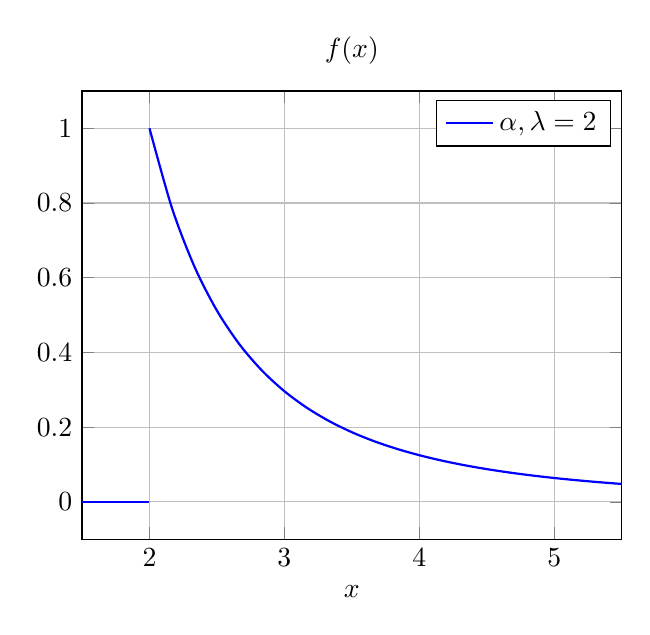
\begin{tikzpicture}
		\begin{axis}[xlabel=$x$, grid = both, xmin = 1.5, xmax = 5.5, title = {$f(x)$}]
			\addplot[thick, smooth, draw=blue][name path = f1, domain = 0:2]{0};
			\addplot[thick, smooth, draw=blue][name path = f1, domain = 2:6]{8/(x^(3))};
			\addlegendentry{$ \alpha, \lambda = 2$}
		\end{axis}
	\end{tikzpicture}
	%
	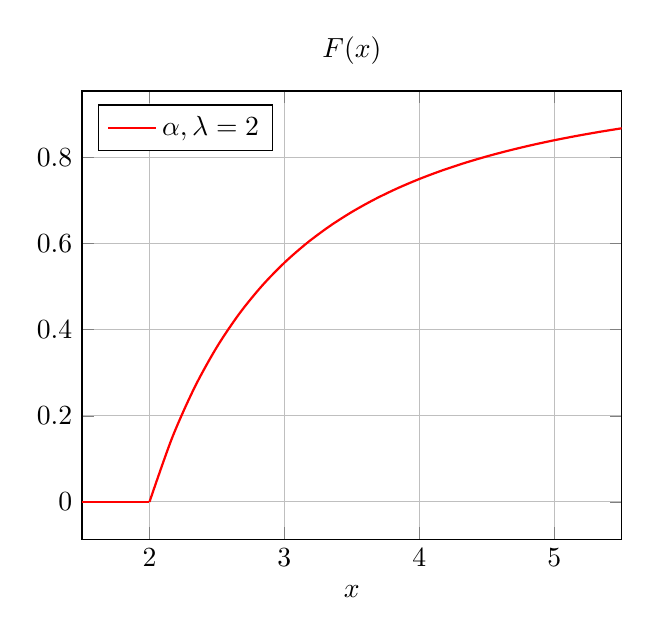
\begin{tikzpicture}
		\begin{axis}[xlabel=$x$, grid = both, xmin = 1.5, xmax = 5.5, title = {$F(x)$}, legend pos = north west]
			\addplot[thick, smooth, draw=red][name path = f1, domain = 0:2]{0};
			\addplot[thick, smooth, draw=red][name path = f1, domain = 2:6]{1 - (2/x)^2};
			\addlegendentry{$ \alpha, \lambda = 2$}
		\end{axis}
	\end{tikzpicture}
\end{figure}

The expected value is finite only for $ \lambda > 1 $,

\begin{align}
	\mathbb{E}(Y) &= \alpha \ \frac{\lambda}{\lambda - 1 }
\end{align}

As a result of the self-similarity of the exponential distribution, the Pareto RV is also self-similar. Given the condition $ Y > y_0 $ for some $ y_0 > \alpha $, this conditional distribution is also Pareto with parameters $ y_0 $ and $ \lambda $.

\begin{align}
	P \left\{Y > y\ |\ Y > y_0 \right\} = \left(\frac{y_0}{y}\right)^\lambda
\end{align}

\textbf{Gamma distribution} : Consider the gamma function $ \Gamma(x) $ defined by an integral which can be recursively related to itself.

\begin{align}
	\Gamma(\alpha) &= \int\limits_{0}^{\infty} e^{-y}\ y^{\alpha -1}\ \mathrm{d}y \\
	%
	\Gamma(\alpha) &= (\alpha - 1)\ \Gamma(\alpha - 1)
\end{align}

For the special case of integer values of $ \alpha $, and using $ \Gamma(1) = 1 $,
\begin{align}
	\Gamma(n) &= (n - 1)\ \Gamma(n - 1) \nonumber \\
	%
	\Gamma(n) &= (n-1)!	
\end{align}

The Gamma RV with parameters $ \alpha, \lambda > 0 $, is now defined using the PDF,

\begin{align}
	f(x) &= \lambda\ e^{- \lambda x}\ \frac{(\lambda x)^{\alpha-1}}{\Gamma(\alpha)} \qquad \forall\ x \geq 0 \\
	%
	&= 0 \qquad \text{otherwise} \nonumber
\end{align}

\begin{figure}[H]
	\centering
	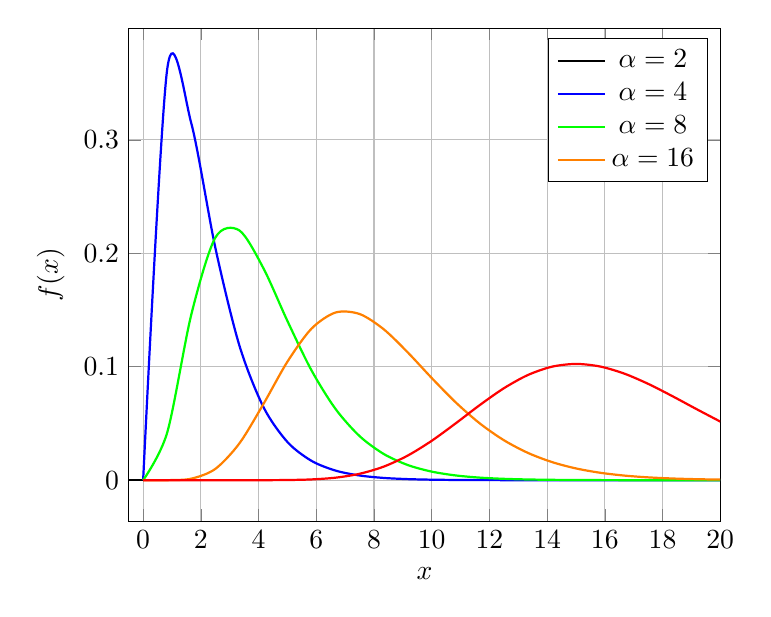
\begin{tikzpicture}
		\begin{axis}[width = 0.75\textwidth,xlabel=$x$, ylabel=$ f(x) $, grid = both, xmin = -0.5, xmax = 20]
			\addplot[thick, smooth, draw=black][name path = f1, domain = -1:0]{0};
			\addplot[thick, smooth, draw=blue][name path = f2, domain = 0:20]{e^(-x)*x};
			\addplot[thick, smooth, draw=green][name path = f3, domain = 0:20]{e^(-x)*(x^3)/6};
			\addplot[thick, smooth, draw=orange][name path = f4, domain = 0:20]{e^(-x)*(x^7)/5040};
			\addplot[thick, smooth, draw=red][name path = f5, domain = 0:20]{e^(-x)*(x^15)/1307674368000};
			\legend{$ \alpha = 2 $, $ \alpha = 4 $, $ \alpha = 8 $, $ \alpha = 16 $}
		\end{axis}
	\end{tikzpicture}
\end{figure}



The moment-generating function gives the mean and variance using

\begin{align}
	\phi(t) &= \left(\frac{\lambda}{\lambda - t}\right)^{\alpha} \\
	%
	\mathbb{E}[X] &= \frac{\alpha}{\lambda} \\
	%
	\mathrm{Var}(X) &= \frac{\alpha}{\lambda^2}
\end{align}

Using the moment-generating function above, the sum of many independent Gamma RVs $ \left\{X_i\right\} $ with parameters $ \left\{\alpha_i\right\} $ and a shared $ \lambda $, then their sum $ X = \sum X_i $ is also a Gamma RV with parameters $ \sum \alpha_i $ and $\lambda$.

This result further simplifies when $ \alpha = 1 $, making the Gamma RVs reduce to exponential RVs with the same rate parameter $ \lambda $. The sum of $ n $ independent exponential RVs $ \left\{X_i\right\} $ with a shared rate $ \lambda $, is a Gamma RV with parameters $ (n, \lambda) $.

Note the effect of multiplying a Gamma RV by a scalar. Let $ X $ be a Gamma RV which is multiplied by scalar $ b $, Now the moment-generating function of the new RV $ bX $ is

\begin{align}
	\mathbb{E}[e^{tX}] &= \left(\frac{\lambda}{\lambda - t}\right)^\alpha \nonumber \\
	%
	\mathbb{E}[e^{t\ bX}] &= \mathbb{E}[e^{bt\ X}] = \left(\frac{\lambda}{\lambda - bt}\right)^\alpha = \left(\frac{\lambda / b}{\lambda / b - t}\right)^\alpha \nonumber \\
	%
	bX &\sim \Gamma(\alpha, \lambda / b)  \qquad \text{if} \qquad X \sim \Gamma(\alpha, \lambda)
\end{align}

\textbf{Chi-square distribution} : Consider a set of independent standard normal RVs $ \left\{Z_i\right\} $. Then the RV defined as $ X \sim \chi_n^2 $ is given by

\begin{align}
	X = Z_1^2 + Z_2^2 + \dots + Z_n^2
\end{align}

$ X $ is a chi-squared RV with $ n $ \textit{degrees of freedom}. Similar to the p-value from the normal RV, $ \chi_{\alpha, n}^2 $ is defined as follows and tabulated using approximate computations.

\begin{align}
	P \left\{X \geq \chi_{\alpha, n}^2 \right\} = \alpha
\end{align}

The equivalence of the chi-squared and Gamma distributions can be seen through the moment-generating functions 

\begin{align}
	\phi(t) &= (1-2t)^{-n/2} \\
	%
	\phi(t) &= \left(\frac{1/2}{1/2 - t}\right)^{n/2} \nonumber
\end{align}

Thus, a chi-squared RV with $ n $ degrees of freedom is the same as a Gamma distribution with parameters $ (n/2, 1/2) $.

\begin{align}
	\mathbb{E}[X] &= \frac{n/2}{1/2} = n \\
	%
	\mathrm{Var}(X) &= \frac{n/2}{(1/2)^2} = 2n
\end{align}

\textbf{t-distribution} : Using a standard normal RV $ Z $ and a chi-square RV $ \chi_n^2 $ with $ n $ degrees of freedom, the t-distribution is defined as,

\begin{align}
	T_n = \frac{Z}{\sqrt{\chi_n^2 / n}}
\end{align}

The t-distribution is also symmetric about $ x=0 $ like $ Z $, but with longer tails. It increasingly resembles $ Z $ as $ n \to \infty $. To prove this, use the weak law of large numbers on the denominator above.

\begin{align}
	\mathbb{E}[X] &= 0 \qquad n>1 \\
	%
	\mathrm{Var}(X) &= \frac{n}{n-2} \qquad n>2
\end{align}

Similar to the p-value from the normal RV, $ t_{\alpha, n} $ is defined as follows and tabulated using approximate computations.

\begin{align}
	P \left\{T_n \geq t_{\alpha, n} \right\} &= \alpha \\
	%
	t_{1-\alpha, n} &= -t_{\alpha, n} \nonumber
\end{align}

\textbf{F-distribution} : Let $ \chi_n^2, \chi_m^2 $ be chi-square RVs with $ n, m $ degrees of freedom respectively. Then,

\begin{align}
	F_{n,m} = \frac{\chi_n^2 / n}{\chi_m^2 / m}
\end{align}

is an F-distribution with$ n,m $ degrees of freedom.

Similar to the p-value from the normal RV, $ F_{\alpha, n, m} $ is defined as follows and tabulated using approximate computations.

\begin{align}
	P \left\{F_{n,m} \geq F_{\alpha, n, m} \right\} &= \alpha \\
\end{align}

\newpage


\chapter{Distributions of Sampling Statistics}


\begin{flushright}
	\textit{``Just find a way to jam it into the Central Limit Theorem"}
\end{flushright}

Most real world populations are intractably large and the statistics of the entire population are impossible to arrive at using brute-force computation. The use of a well-drawn sample to estimate the statistics of the underlying population is the most-used workaround to this problem.

\textbf{Random sample} : A set of random variables which are independent and have a common distribution $ F $. When $ F $ is only specified up to some parameters that are not known, it is possible to estimate these parameters using the statistics of the random sample.

Depending on whether any information about the form of $ F $ is known, this is called either a  \textit{parametric} inference problem, or a \textit{non-parametric} inference problem. An example of the latter is knowing only whether $ F $ is continuous or discrete and nothing further.

\textbf{Statistic} : A RV which is determined by the random sample instead of the underlying population. The two most interesting statistics are the sample mean and the sample variance.

\textbf{Sample mean} : Consider a population with mean $ \mu $ and variance $ \sigma $, without any information about the specific probability distribution. In contrast to the population mean and variance, the \textit{sample mean} of a random sample $ \left\{X_i\right\} $ is defined as

\begin{align}
	\overline{X} &= \frac{X_1 + X_2 + \dots + X_n}{n}
\end{align}

$ \overline{X} $ is also an RV, whose expected value and variance are

\begin{align}
	\mathbb{E}[\overline{X}] &= \frac{1}{n}\ \left(\mathbb{E}[X_1] + \dots + \mathbb{E}[X_n]\right) = \mu \\
	%
	\mathrm{Var}(\overline{X}) &= \frac{1}{n^2}\ \left[\mathrm{Var}(X_1) + \dots + \mathrm{Var}(X_n)\right] = \frac{\sigma^2}{n}
\end{align}

The sample mean from an underlying standard normal population for different values of sample size, is itself a normal RV with spread decreasing as $ n $ increases.

\begin{figure}[H]
	\centering
	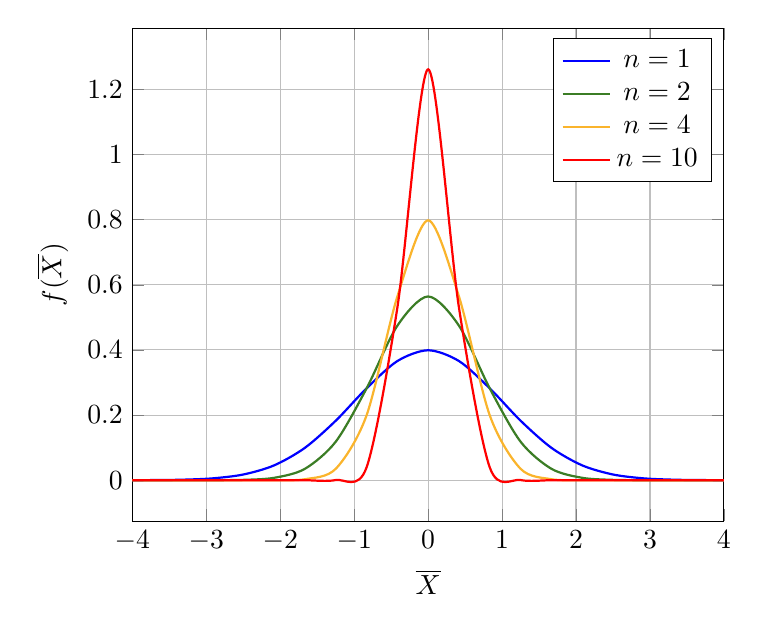
\begin{tikzpicture}
		\begin{axis}[width = 0.75\textwidth,xlabel=$\overline{X}$, ylabel=$ f(\overline{X}) $, grid = both, xmin = -4, xmax = 4]
			\addplot[thick, smooth, draw=blue][name path = f2, domain = -5:5]{(1/sqrt(2*pi))*e^(-0.5*x*x)};
			\addplot[thick, smooth, draw=OliveGreen][name path = f3, domain = -5:5]{(1/sqrt(pi))*e^(-0.5*2*x*x)};
			\addplot[thick, smooth, draw=Dandelion][name path = f4, domain = -5:5]{(1/sqrt(0.5*pi))*e^(-0.5*4*x*x)};
			\addplot[thick, smooth, draw=red][name path = f5, domain = -5:5]{(1/sqrt(0.2*pi))*e^(-0.5*10*x*x)};
			\legend{$n=1$,$n=2$,$n=4$, $n=10$}
		\end{axis}
	\end{tikzpicture}
\end{figure}

\textbf{Central Limit Theorem} : Let $ \left\{X_i\right\} $ be independent identically distributed RV having the same mean $ \mu $ and variance $ \sigma^2 $.

In the limit of large $ n $, the distribution of $ \sum X_i $ is approximately normal with mean $ n\mu $ and variance $ n\sigma^2 $, regardless of the probability distribution of the individual $ X_i $ 

\begin{align}
	\frac{X_1 + X_2 + \dots + X_n - n\mu}{\sqrt{n}\ \sigma} &\sim Z
\end{align}

Consider the specific case of a binomial RV with parameters $ (n, p) $. This is decomposed into a set of $ n $ binary indicator RVs. Then for large $ n $,

\begin{align}
	X &= X_1 + X_2 + \dots + X_n \nonumber \\
	%
	\mathbb{E}[X_i] &= p \nonumber \\
	%
	\mathrm{Var}(X_i) &= (1-p) \nonumber \\
	%
	\frac{X - np}{\sqrt{np(1-p)}} & \sim Z 
\end{align}

\begin{figure}[!h]
	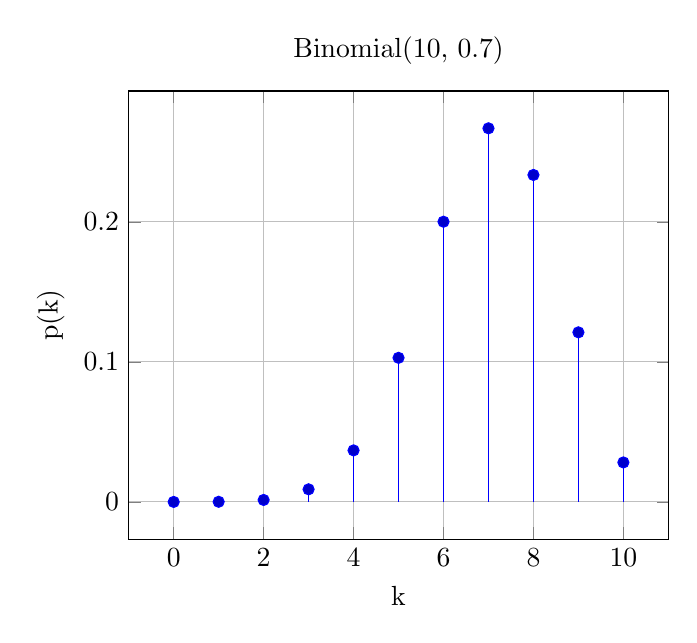
\begin{tikzpicture}
		\begin{axis}[grid = both,
			xlabel = k, ylabel = p(k), title = {Binomial(10, 0.7)}]
			\addplot+[ycomb] plot coordinates {( 0 , 0.0 ) ( 1 , 0.0001 ) ( 2 , 0.0014 ) ( 3 , 0.009 ) ( 4 , 0.0368 ) ( 5 , 0.1029 ) ( 6 , 0.2001 ) ( 7 , 0.2668 ) ( 8 , 0.2335 ) ( 9 , 0.1211 ) ( 10 , 0.0282 ) 
			 };  
		\end{axis} 
	\end{tikzpicture}
	%
	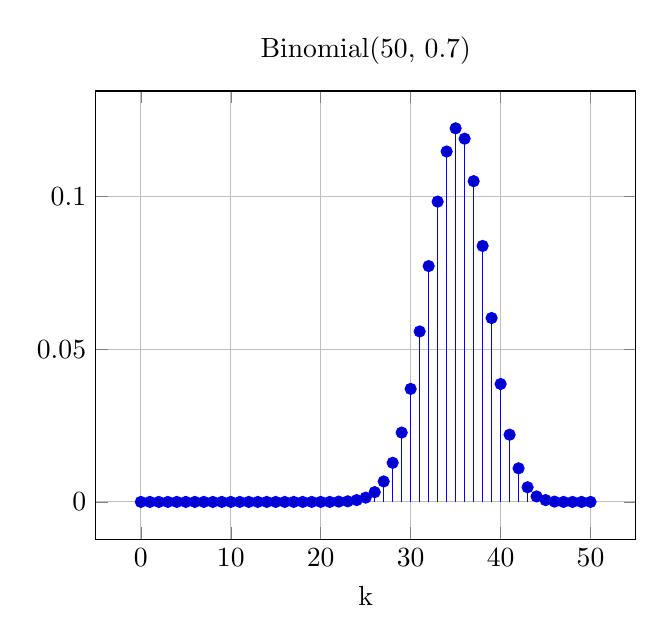
\begin{tikzpicture}
		\begin{axis}[grid = both, yticklabel style={
				/pgf/number format/fixed,
				/pgf/number format/precision=2
			},
			xlabel = k, title = {Binomial(50, 0.7)}]
			\addplot+[ycomb] plot coordinates {( 0 , 0.0 ) ( 1 , 0.0 ) ( 2 , 0.0 ) ( 3 , 0.0 ) ( 4 , 0.0 ) ( 5 , 0.0 ) ( 6 , 0.0 ) ( 7 , 0.0 ) ( 8 , 0.0 ) ( 9 , 0.0 ) ( 10 , 0.0 ) ( 11 , 0.0 ) ( 12 , 0.0 ) ( 13 , 0.0 ) ( 14 , 0.0 ) ( 15 , 0.0 ) ( 16 , 0.0 ) ( 17 , 0.0 ) ( 18 , 0.0 ) ( 19 , 0.0 ) ( 20 , 0.0 ) ( 21 , 0.0 ) ( 22 , 0.0001 ) ( 23 , 0.0002 ) ( 24 , 0.0006 ) ( 25 , 0.0014 ) ( 26 , 0.0032 ) ( 27 , 0.0067 ) ( 28 , 0.0128 ) ( 29 , 0.0227 ) ( 30 , 0.037 ) ( 31 , 0.0558 ) ( 32 , 0.0772 ) ( 33 , 0.0983 ) ( 34 , 0.1147 ) ( 35 , 0.1223 ) ( 36 , 0.1189 ) ( 37 , 0.105 ) ( 38 , 0.0838 ) ( 39 , 0.0602 ) ( 40 , 0.0386 ) ( 41 , 0.022 ) ( 42 , 0.011 ) ( 43 , 0.0048 ) ( 44 , 0.0018 ) ( 45 , 0.0006 ) ( 46 , 0.0001 ) ( 47 , 0.0 ) ( 48 , 0.0 ) ( 49 , 0.0 ) ( 50 , 0.0 ) 
			};  
		\end{axis} 
	\end{tikzpicture}
\end{figure} 

While the Poisson approximation to a Binomial RV is good for large $ n $ and small $ p $, this normal approximation is only good for large values of $ \sqrt{np(1-p)} $, with this value by convention being $ \geq 10 $.

The sample mean also obeys the central limit theorem for large values of sample size $ n $ to give,

\begin{align}
	\frac{\overline{X} - \mu}{\sigma / \sqrt{n}} &\sim Z
\end{align}

By convention, a sample size of at least $ 30 $ is needed to ensure that the sample mean will be approximately normal regardless of the underlying probability distribution. This minimum sample size is much smaller for specific distributions such as a normal RV ($ n \geq 1 $) and an exponential RV ($ n \geq 5 $)


\begin{figure}[H]
	\centering
	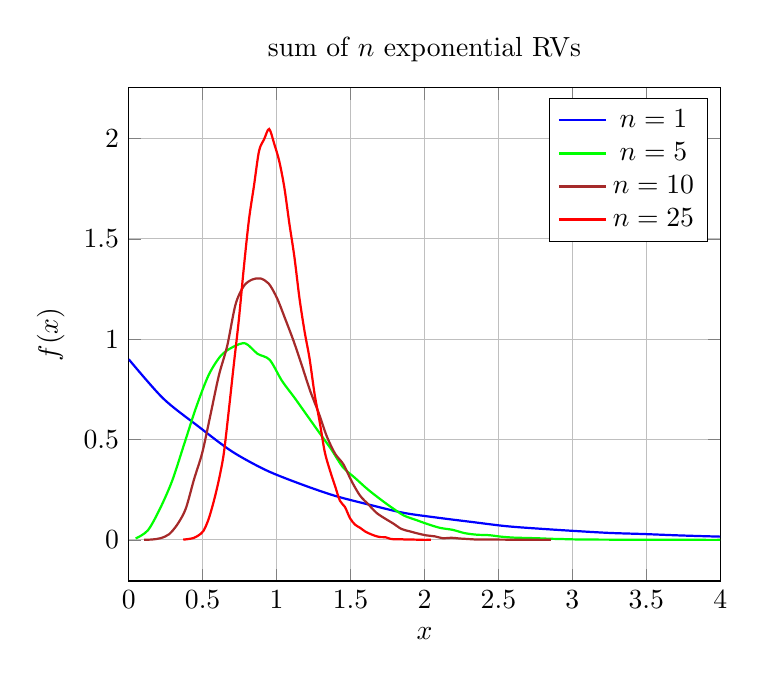
\begin{tikzpicture}
	\begin{axis}[width = 0.75\textwidth,grid = both, xmax = 4.0, xmin = 0,
		xlabel = $ x $, ylabel=$ f(x) $, title = sum of $ n $ exponential RVs]

		\addplot[smooth, thick, color = blue] plot coordinates {
			(0.0, 0.9003) (0.2322, 0.7054) (0.4643, 0.5692) (0.6965, 0.4414) (0.9286, 0.3473) (1.1607, 0.2788) (1.3929, 0.2199) (1.625, 0.1757) (1.8572, 0.1349) (2.0893, 0.1105) (2.3215, 0.0891) (2.5536, 0.0682) (2.7858, 0.0553) (3.0179, 0.0443) (3.2501, 0.0346) (3.4822, 0.0291) (3.7144, 0.0224) (3.9465, 0.0172) (4.1787, 0.013) (4.4108, 0.0109) (4.643, 0.0083) (4.8751, 0.0069) (5.1073, 0.0053) (5.3394, 0.0037) (5.5716, 0.0036) (5.8037, 0.0027) (6.0359, 0.0019) (6.268, 0.0015) (6.5002, 0.0012) (6.7323, 0.0009) (6.9645, 0.0009) (7.1966, 0.0006) (7.4288, 0.0006) (7.6609, 0.0002) (7.8931, 0.0002) (8.1252, 0.0002) (8.3574, 0.0002) (8.5895, 0.0003) (8.8217, 0.0001) (9.0538, 0.0002) (9.286, 0.0001) (9.5181, 0.0002) (9.7502, 0.0) (9.9824, 0.0) (10.2145, 0.0001) (10.4467, 0.0) (10.6788, 0.0) (10.911, 0.0) (11.1431, 0.0) (11.3753, 0.0001)
			
		}; 
		\addplot[smooth, thick, color = green] plot coordinates {
			(0.0473, 0.007) (0.1297, 0.0475) (0.2121, 0.1563) (0.2945, 0.2957) (0.3769, 0.4815) (0.4593, 0.6674) (0.5417, 0.823) (0.6241, 0.9185) (0.7064, 0.9618) (0.7888, 0.9792) (0.8712, 0.9273) (0.9536, 0.897) (1.036, 0.7929) (1.1184, 0.7112) (1.2008, 0.6257) (1.2832, 0.5401) (1.3656, 0.4557) (1.448, 0.3626) (1.5304, 0.3085) (1.6128, 0.254) (1.6952, 0.206) (1.7776, 0.1617) (1.86, 0.1217) (1.9424, 0.0994) (2.0248, 0.0776) (2.1071, 0.0595) (2.1895, 0.0501) (2.2719, 0.0336) (2.3543, 0.0257) (2.4367, 0.0234) (2.5191, 0.0159) (2.6015, 0.0113) (2.6839, 0.0096) (2.7663, 0.008) (2.8487, 0.0055) (2.9311, 0.004) (3.0135, 0.0024) (3.0959, 0.0022) (3.1783, 0.0013) (3.2607, 0.0011) (3.3431, 0.0007) (3.4255, 0.0007) (3.5078, 0.0006) (3.5902, 0.0001) (3.6726, 0.0006) (3.755, 0.0004) (3.8374, 0.0004) (3.9198, 0.0) (4.0022, 0.0001) (4.0846, 0.0002)
		}; 
		\addplot[smooth, thick, color = Brown] plot coordinates {
			(0.1048, 0.0005) (0.1609, 0.002) (0.2171, 0.0087) (0.2732, 0.0282) (0.3293, 0.0773) (0.3854, 0.1545) (0.4416, 0.3015) (0.4977, 0.4353) (0.5538, 0.6265) (0.6099, 0.82) (0.666, 0.9665) (0.7222, 1.1726) (0.7783, 1.2649) (0.8344, 1.2972) (0.8905, 1.3027) (0.9467, 1.2772) (1.0028, 1.2049) (1.0589, 1.1001) (1.115, 0.991) (1.1711, 0.8686) (1.2273, 0.742) (1.2834, 0.635) (1.3395, 0.516) (1.3956, 0.4294) (1.4518, 0.3765) (1.5079, 0.2915) (1.564, 0.2209) (1.6201, 0.1771) (1.6763, 0.1342) (1.7324, 0.1066) (1.7885, 0.0816) (1.8446, 0.0542) (1.9007, 0.0424) (1.9569, 0.0314) (2.013, 0.0223) (2.0691, 0.0176) (2.1252, 0.008) (2.1814, 0.0105) (2.2375, 0.0068) (2.2936, 0.0043) (2.3497, 0.0018) (2.4058, 0.0023) (2.462, 0.0018) (2.5181, 0.0012) (2.5742, 0.0011) (2.6303, 0.0009) (2.6865, 0.0002) (2.7426, 0.0002) (2.7987, 0.0) (2.8548, 0.0004)
		};
		\addplot[smooth, thick, color = red] plot coordinates {
			(0.3687, 0.0012) (0.4029, 0.0041) (0.4371, 0.0091) (0.4712, 0.0219) (0.5054, 0.0448) (0.5396, 0.1021) (0.5738, 0.1884) (0.6079, 0.2929) (0.6421, 0.4258) (0.6763, 0.6417) (0.7105, 0.8726) (0.7446, 1.0961) (0.7788, 1.3592) (0.813, 1.595) (0.8472, 1.7651) (0.8813, 1.938) (0.9155, 1.9959) (0.9497, 2.0477) (0.9839, 1.9737) (1.018, 1.8871) (1.0522, 1.7569) (1.0864, 1.5763) (1.1206, 1.4089) (1.1547, 1.2044) (1.1889, 1.04) (1.2231, 0.903) (1.2573, 0.7251) (1.2914, 0.5879) (1.3256, 0.4386) (1.3598, 0.3485) (1.394, 0.2718) (1.4281, 0.1955) (1.4623, 0.1639) (1.4965, 0.108) (1.5307, 0.0758) (1.5648, 0.06) (1.599, 0.0418) (1.6332, 0.0296) (1.6674, 0.0199) (1.7015, 0.0138) (1.7357, 0.0132) (1.7699, 0.005) (1.804, 0.0029) (1.8382, 0.0035) (1.8724, 0.0015) (1.9066, 0.0015) (1.9407, 0.0012) (1.9749, 0.0003) (2.0091, 0.0) (2.0433, 0.0006)
			
		};
	\legend{$n=1$,$n=5$,$n=10$, $n=25$}		
	\end{axis} 
	\end{tikzpicture}
\end{figure} 

\textbf{Sample variance} : Using the prior definition of the variance $ S^2 $, a sample drawn from an underlying distribution with parameters $ \mu, \sigma $ and sample mean $ \overline{X} $ has the sample variance $ S^2 $ defined as,

\begin{align}
	S^2 &= \ddfrac{\sum\limits_{i=1}^{n}(X_i - \overline{X})^2}{n-1}
\end{align}

The expected value of the sample variance is found using,

\begin{align}
	\sum\limits_{i=1}^{n}(x_i - \overline{x})^2 &= \sum\limits_{i=1}^{n}(x_i^2) - n\overline{x}^2 \nonumber \\
	%
	\mathbb{E}[X^2] &= \mathrm{Var}(X) + (\mathbb{E}[X])^2 \nonumber 
\end{align}

The derivation of $ \mathbb{E}[S^2] $, using the above relations is as follows,

\begin{align}
	(n-1)\mathbb{E}[S^2] &= \mathbb{E}\left[\sum\limits_{i=1}^{n}X_i^2\right] - n\mathbb{E}[\overline{X}^2] \nonumber \\
	%
	&= n\left[\mathrm{Var}(X_1) + (\mathbb{E}[X_1])^2 - \mathrm{Var}(\overline{X}) - (\mathbb{E}[\overline{X}])^2\right] \nonumber \\
	%
	&= n\sigma^2 + n\mu^2 - n(\sigma^2/n) - n\mu^2 \nonumber \\
	%
	\mathbb{E}[S^2] &= \sigma^2
\end{align}

\textbf{Sampling from a normal population} : For the specific case of samples drawn from an underlying population which is normally distributed $ X_i \sim \mathcal{N}(\mu, \sigma^2) $, the distribution of the sample mean and sample variance is of particular interest for real-world applications.

The sample mean $ \overline{X} $ is itself a normal RV, with mean $ \mu $ and variance $ \sigma^2 / n $ 

The sample variance is independent from the sample mean exclusively when the underlying population is a normal RV, with

\begin{align}
	\frac{(n-1)}{\sigma^2}\ S^2 &\sim \chi^2_{n-1}
\end{align}

As a corollary to the above, a t-distribution with $ (n-1) $ DOF, can be observed from the following combination of the sample mean and sample variance,

\begin{align}
	\frac{\overline{X}- \mu}{\sigma / \sqrt{n}}\ \sqrt{\frac{\sigma^2}{S^2}} &\sim \frac{Z}{\sqrt{\chi^2_{n-1} / (n-1)}} \nonumber \\
	%
	\frac{\sqrt{n}\ (\overline{X}- \mu)}{S} &\sim t_{n-1}
\end{align}

\textbf{Sampling from finite population} : Consider a population of size $ N $, which has a proportion $ p $ of its elements possessing a certain property of interest. A random sample of size $ n $ picked from this population would be equally likely to be any of the possible binomial combinations.

The most common method of successively generating a random sample is to simply select one of the remaining members of the population at random at each step until the desired sample size is reached.

A set of binary indicator RVs $ \left\{X_i\right\} $ which indicate whether the $ i^{th} $ member of the sample possesses the property of interest would then sum up to $ X = \sum X_i $. Note that these $ X_i $ are not independent. Independence of the $ X_i $ is a valid assumption only for $ N \ggg n $

\begin{align}
	P\left\{X_i = 1\right\} &= p \qquad \text{and} \qquad P\left\{X_i = 0\right\} = (1-p)
\end{align}

The sample mean $ \overline{X} $ is the proportion of the sample that has the property of interest. In the limit of large $ N $, $ X $ becomes a binomial RV with parameters $ (n, p) $.

When the sample is not a very small fraction of the population, $ X $ is a hyper-geometric random variable with parameters $ (Np, N(1-p), n) $

Proceeding with the $ N \ggg n $ approximation, $ X $ reduces to a binomial RV.

\begin{align}
	\mathbb{E}[\overline{X}] &= p \\
	%
	\mathrm{Var}(\overline{X}) &= \frac{p(1-p)}{n}
\end{align}


\chapter{Parameter Estimation}


\begin{flushright}
	\textit{``Please explain in detail your reasons for choosing this prior distribution"}
\end{flushright}

Consider a distribution $ F_\theta $ from which a random sample $ \left\{X_i\right\} $ is drawn. It is an extremely common problem to estimate the vector of parameters $ \theta $ of the underlying distribution using only the information from the sample.

Estimates of these parameters can either be provided as a \textit{point} or an \textit{interval}, alongside a \textit{confidence} value associated with these estimates.

An important class of such problems is \textit{Bayesian estimation}, which involves estimating an unknown parameter only partial information about it is known.

\textbf{Maximum Likelihood Estimator} : An estimator of an unknown parameter $ \theta $ is any sample-derived statistic used to estimate its value. The observed value of an estimator is called the \textit{estimate}.

As an example consider $ n $ random samples drawn from an underlying exponential distribution whose mean is the unknown parameter $ \theta $. The joint PDF of the RVs $ \left\{X_i\right\} $, which would then be used to estimate $ \theta $ is given by

\begin{align}
	f(x_1, x_2, \dots, x_n) &= f_{x_1} (X_1)\ f_{X_2} (2_1)\ \dots\  f_{X_n} (x_n) \nonumber \\
	%
	&= \frac{1}{\theta} e^{-x_1/\theta} \ \frac{1}{\theta} e^{-x_2/\theta} \dots \ \frac{1}{\theta} e^{-x_n/\theta} \qquad x_i > 0 \nonumber \\
	%
	&= \frac{1}{\theta^n}\ \exp \left\{ \sum_{i=1}^{n} \frac{-x_i}{\theta} \right\}
\end{align}

\textit{Likelihood function} : Define $ f(x_1, x_2,\dots,x_n\ |\ \theta) $ as the joint PDF or PMF of the $ n $ random samples from an underlying distribution with unknown parameter $ \theta $. This term is the likelihood that the values $ \left\{ x_i \right\} $ will actually be observed when $ \theta $ is the true value of the parameter.

The \textit{maximum likelihood estimate} $ \widehat{\theta} $ is that value of the parameter $ \theta $ which maximizes the likelihood function. A useful computational convenience is that log likelihood also has its maximum at the same point as likelihood itself.

The algorithm usually involves identifying the likelihood function after incorporating the unknown parameter $ \theta $, taking logarithm wherever convenient, and then differentiating with respect to $ \theta $ in order to maximize the likelihood.

A sample of size $ n $ from an underlying Bernoulli distribution whose unknown mean $ p $ is to be estimated. The above procedure yields the maximum likelihood estimator of $ p $ to be the sample mean $ \sum X_i / n$.

The above problem when the underlying distribution is Poisson with rate $ \lambda $ yields the MLE as $ \widehat{\lambda} =  \sum X_i / n$.

However, for a uniform distribution on $ [0, \theta] $, the parameter is estimated by $ \widehat{\theta} = \max(\left\{X_i\right\}) $ and not by the sample mean.

The more relevant problem is with an underlying normal distribution with unknown $ \mu $ and $ \sigma $, to be estimated using a sample of size $ n $.

\begin{align}
	\widehat{\mu} = \frac{1}{n}\ \sum\limits_{i=1}^{n} x_i = \overline{X} \qquad \text{and} \qquad \widehat{\sigma} = \left[\frac{1}{n}\  \sum\limits_{i=1}^{n} (X_i - \overline{X})^2 \right] ^{1/2} \\
\end{align}

Note that $ \widehat{\sigma} $ differs from the sample standard deviation $ S $, in the denominator being $ n $ instead of $ (n-1) $.

\textit{Failure and survival rate} : Defining failure rate $ \lambda_i $ and survival rate $ s_i = 1 - \lambda_i $ for an underlying discrete distribution taking values $ i \geq 1 $,

\begin{align}
	\lambda_i &= P \left\{X = i\ |\ X > i-1\right\} = \frac{P \left\{X = i\right\}}{P\left\{X > i-1\right\}} \\
	%
	s_i &= 1 - \lambda_i = \frac{P \left\{X > i\right\}}{P\left\{X > i-1\right\}}
\end{align}

For illustration, let $ X $ denote a human's age at death. Now, failure rate is a measure of the fraction of all people surviving at least $ i-1 $ years who will die at age $ i $.

Using the relations,

\begin{align}
	P \left\{X > i\right\} &= s_1\ s_2\ \dots\ s_i \nonumber \\
	%
	P\left\{X = n\right\} &= \lambda_n\ P \left\{X > n-1\right\} = s_1\ s_2\ \dots\ s_{n-1}\ (1 - s_n) 
\end{align}

Using the above PMF for $ X $ requires estimating the survival rates $ \widehat{s_i} $. This is a simple task of looking at what fraction of the sample who reached age $ i $ one year ago are alive today.

\textbf{Interval estimates} : It is often useful to provide an interval for the estimate of a parameter along with an associated confidence value instead of just a point value. This involves looking at the probability distribution of the estimator itself.

As an example, consider the MLE of the mean of a normal RV from which a sample of size $ n $ is drawn. The MLE $ \overline{X} $ is known to have a normal distribution with mean $ \mu $ and variance $ \sigma^2 / n $.

Rearranging the sample mean to form a standard normal RV $ Z $, and using its CDF to find a $ 95\% $ confidence interval gives,

\begin{align}
	\frac{\overline{X} - \mu}{\sigma / \sqrt{n}} &\sim Z \nonumber \\
	%
	P \left\{ | \overline{X} - \mu | \leq \frac{1.96\ \sigma}{\sqrt{n}} \right\} &= 0.95 \nonumber \\
	%
	\text{with 95 \% confidence, } \mu &\in \left[ \overline{x} - \frac{1.96\ \sigma}{\sqrt{n}}, \ \overline{x} + \frac{1.96\ \sigma}{\sqrt{n}} \right]
\end{align}

The above relation states that if the sample mean $ \overline{X} = \overline{x} $, then the population mean $ \mu $ lies within this interval with $ 95\% $ confidence.

In addition to the \textit{two-sided} confidence interval for $ \mu $ above, the \textit{one-sided upper} and \textit{one-sided lower} $ 95\% $ confidence intervals for $ \mu $ are,

\begin{align}
	\mu \in \left[ \overline{x} - \frac{1.645\ \sigma}{\sqrt{n}}\ ,\  \infty \right) \qquad \text{and} \qquad \mu \in \left( -\infty\ ,\  \overline{x} + \frac{1.645\ \sigma}{\sqrt{n}} \right]
\end{align}

The factors of $ 1.96 $ and $ 1.645 $ used above were obatined using the inverse CDF of the normal distribution for $ p = 0.975 $ and $ p = 0.95 $ respectively. A different confidence interval would involve recalculating the inverse CDF and replacing the pre-factors used above.

\textit{Confidence interval for a normal mean with unknown variance} : Consider a normal RV with unknown $ \mu $ and $ \sigma $, from which a sample of size $ n $ is drawn. Since the above procedure can no longer be used to construct confidence intervals, the sample variance $ S $ is now of interest.

Using the fact that $ \sqrt{n}(\overline{X} - \mu) / S \sim t_{n-1}$, and the symmetry of the t-distribution, for some observed value of sample mean and variance $ \overline{x}, s^2 $


\begin{align}
	1 - \alpha &= P \left\{ | \overline{X} - \mu | \leq \frac{t_{\alpha/2, n-1}\ S}{\sqrt{n}} \right\}  \nonumber \\
	%
	\mu &\in \left[ \overline{x} - \frac{(t_{\alpha/2, n-1})\ s}{\sqrt{n}}, \ \overline{x} + \frac{(t_{\alpha/2, n-1})\ s}{\sqrt{n}} \right]
\end{align}

This becomes the $ 100(1-\alpha) \% $ confidence interval for $ \mu $. As $ n \to \infty $, the t-distribution reduces to the standard normal and the the new confidence interval expression reduces to the old one. It is common, but not necessary that the confidence interval when $ \sigma $ is unknown is larger than when it is known, by virtue of the t-distribution being wider than the standard normal distribution, and the general trend of $ S^2 > \sigma^2 $.

The above methods have assumed an underlying normal distribution. However, for a large enough sample size, they may be used even when the underlying PDF is not a normal RV because of the Central Limit theorem.


\textit{Monte-Carlo simulation} : The process of randomly sampling from a uniform distribution to estimate difficult integrals using the power of the central limit theorem acting on a large sample consisting of \texttt{i.i.d.} RVs.

For example, consider a set of $ n $ uniform RVs $ \left\{U_i\right\} $ in the domain $ [a,b] $ 

\begin{align}
	\theta = \int\limits_{a}^{b}\ g(x)\ \mathrm{d}x = \mathbb{E}[g(x)]
\end{align}

A new set of RVs $ \left\{X_i\right\}  = g(\left\{U_i\right\})$, which are random samples drawn from the PDF $ g(x) $, would now have sample mean and variance $ \overline{x} $ and $ s^2 $. A confidence interval for $ \mathbb{E}[g(x)] $ is now constructed using the t-distribution method described above. 

\textit{Prediction Interval} : The problem of predicting a confidence interval for the next sample $ X_{n+1} $ drawn from a normal distribution with parameters $ \mu, \sigma $ given a set of $ n $ samples already available, is similar to the above procedure.

Let $ S_n^2 $ and $ \overline{X}_n $ be the sample variance and mean using the first $ n $ samples. Since $ \overline{X}_n $ is a normal RV with mean $ \mu $ and variance $ \sigma^2 / n $, whereas $ X_{n+1} $ is also a normal RV independent of $ \overline{X}_n $ ,


\begin{align}
	\frac{X_{n+1} - \overline{X}_n}{\sigma \sqrt{1 + 1/n}} &\sim Z \nonumber \\
	%
	\frac{X_{n+1} - \overline{X}_n}{S_n \sqrt{1 + 1/n}} &\sim t_{n-1} \nonumber \\
\end{align}

Once again, this leads to the confidence intervals using the t-distribution defined above.

\textit{Confidence interval for a normal variance with unknown mean} : Using the fact that $ (n-1) S^2 / \sigma^2 \sim \chi^2_{n-1} $, the $ 100(1-\alpha) \% $ confidence interval for a sample of size $ n $ with sample variance $ S^2 = s^2 $ is calculated as,

\begin{align}
	\sigma^2 &\in \left[\ddfrac{(n-1)s^2}{\chi^2_{\alpha/2, n-1}}\ ,\ \frac{(n-1)s^2}{\chi^2_{1 - \alpha/2, n-1}}\right]
\end{align}

Note the use of $ \chi^2_{\alpha/2, n-1} $ as well as $ \chi^2_{1 - \alpha/2, n-1} $ arising from the fact that the $ \chi_n^2 $ distribution is not symmetric about its mean.

\textbf{Difference in means of two normal populations} : The problem is to estimate $ \mu_1 - \mu_2 $, where two normal RVs $ X, Y $ with means $ \mu_1, \mu_2 $ and variances $ \sigma_1^2, \sigma_2^2 $ respectively are used to generate two sets of samples $ \left\{X_1, \dots, X_n\right\} $ and $ \left\{Y_1, \dots, Y_m\right\} $.

Additionally, the sample sets $ \left\{X_i\right\}, \left\{Y_j\right\} $ are independent.

The point estimator of $ \mu_1 - \mu_2 $ is simply $ \overline{X} - \overline{Y} $, using the previous section. For an interval estimate, the distribution of $ \overline{X} - \overline{Y} $ is needed.

\begin{align}
	\overline{X} - \overline{Y} &\sim \mathcal{N}\left(\mu_1 - \mu_2\ ,\ \frac{\sigma_1^2}{n} + \frac{\sigma_2^2}{m}\right) \nonumber \\
	%
	Z &\sim \ddfrac{\overline{X} - \overline{Y} - (\mu_1 - \mu_2)}{\sqrt{\frac{\sigma_1^2}{n} + \frac{\sigma_2^2}{m}}} 
\end{align}

When the variances $ \sigma_1^2, \sigma_2^2 $ are known, the $ 100(1-\alpha)\% $ confidence interval is,

\begin{align}
	\mu_1 - \mu_2 &\in \left[ \overline{x} - \overline{y} - z_{\alpha / 2} \sqrt{\frac{\sigma_1^2}{n} + \frac{\sigma_2^2}{m}}\ ,\ \overline{x} - \overline{y} + z_{\alpha / 2} \sqrt{\frac{\sigma_1^2}{n} + \frac{\sigma_2^2}{m}} \right] 
\end{align}


Next, consider the special case where $ \sigma_1, \sigma_2 $ are unknown but happen to be equal. Now, using the sample variances $ S_1^2, S_2^2 $, and the additive property of chi-squared distributions, the \textit{pooled estimator} $ S_P^2 $ of this common variance is

\begin{align}
	S_P^2 = \frac{(n-1)\ S_1^2 + (m-1)\ S_2^2}{(n+m-2)} \nonumber
\end{align}

Rearranging the sample statistics into a t-distribution after replacing $ \sigma $ with $ S_P $,

\begin{align}
	Z &\sim \frac{\overline{X} - \overline{Y} - (\mu_1 - \mu_2)}{\sqrt{\sigma^2(1/n + 1/m)}} \nonumber \\
	%
	\chi^2_{n+m-2} &\sim (n+m-2)\ \frac{S_P^2}{\sigma^2} \nonumber \\
	%
	t_{n+m-2} &\sim \frac{\overline{X} - \overline{Y} - (\mu_1 - \mu_2)}{\sqrt{S_P^2(1/n + 1/m)}}
\end{align}

Now, the confidence interval is defined using this t-distribution as


\begin{align}
	\mu_1 - \mu_2 &\in \left[ \overline{x} - \overline{y} - t_{\alpha / 2, n+m-2}\ s_p\ \sqrt{\frac{1}{n} + \frac{1}{m}}\ ,\ \overline{x} - \overline{y} + t_{\alpha / 2, n+m-2}\ s_p\ \sqrt{\frac{1}{n} + \frac{1}{m}} \right] 
\end{align}

\textbf{Mean of a Bernoulli RV - confidence interval} : Consider a sample of size $ n $ drawn from a Bernoulli RV with parameter $ p $. The point estimate for $ p $ is simply $ \widehat{p} = \sum X_i / n $.

For an interval estimate, assume $ X = \sum X_i $ has the observed value $ x $, and define the confidence interval for $ p $ as,

\begin{align}
	Z &\sim \frac{X - np}{\sqrt{n \widehat{p} (1 - \widehat{p})}} \nonumber \\
	%
	p &\in \left[ \widehat{p} - z_{\alpha/2}\sqrt{\frac{\widehat{p}(1-\widehat{p})}{n}}\ ,\ \widehat{p} + z_{\alpha/2}\sqrt{\frac{\widehat{p}(1-\widehat{p})}{n}}  \right]
\end{align}

For a given interval of width $ b $ in the above relation, the number of samples required $ n $ is given by

\begin{align}
	b &= 2 z_{\alpha/2}\ \sqrt{\frac{\widehat{p}(1-\widehat{p})}{n}} \qquad \text{and} \qquad n = (2z_{\alpha/2})^2\  \frac{\widehat{p}(1-\widehat{p})}{b^2}
\end{align}

To guarantee a confidence interval of size $ b $ or smaller, the minimum number of samples needed is $ n^* = (Z_{\alpha/2} / b)^2 $ 

\textbf{Mean of exponential distribution - confidence interval} : Consider a set of samples $ \left\{X_1, \dots, X_n\right\} $ drawn from an exponential RV with unknown mean $ \theta $. The point estimate for $ \theta $ is just the sample mean $ \overline{X} $.

For an interval estimate, consider the following RV transformations,

\begin{align}
	\sum X_i &\sim \Gamma(n, 1/\theta) \nonumber \\
	%
	\frac{2}{\theta}\ \sum X_i &\sim \Gamma(n, 1/2) \sim \chi^2_{2n}
\end{align}

Using the above chi-squared distribution, the confidence interval for $ \theta $ is given by,

\begin{align}
	\theta \in \left[\ddfrac{2 \sum X_i}{\chi^2_{\alpha/2, 2n}}\ ,\ \ddfrac{2 \sum X_i}{\chi^2_{1 - \alpha/2, 2n}}\right]
\end{align}

\textbf{Evaluating point estimators} : The question of how good a proposed point estimator $ d(\textbf{X}) $ for a parameter $ \theta $ drawn from a sample $ \textbf{X} = \left\{X_1, \dots, X_n\right\} $ is often answered by looking at the mean squared error $ r(d, \theta) $ 

\begin{align}
	r(d, \theta) = \mathbb{E}[(d(X) - \theta)^2] 
\end{align}

Generally, there is no universal value of $ d $ that minimizes the error above for all values of $ \theta $.


\textit{Bias of an estimator} : For the definitions used above, the bias $ b_{\theta}(d) $ is expressed as,

\begin{align}
	b_\theta (d) = \mathbb{E}[d(\textbf{X})] - \theta
\end{align}

If an estimator has $ 0 $ bias for all values of $ \theta $, then it is called an \textit{unbiased} estimator of $ \theta $. For example, a weighted sum of the random samples from an unknown distribution with mean $ \theta $ is always an unbiased estimator.

\begin{align}
	\mathbb{E}\left[ \sum \lambda_i X_i \right] &= \sum \mathbb{E}[X_i]\ \lambda_i \nonumber \\
	%
	&= \theta\ \sum \lambda_i = \theta \nonumber \\
	%
	\text{if } \sum \lambda_i &= 1
\end{align}

The mean squared error of an unbiased estimator is equal to its variance.

\begin{align}
	r(d, \theta) &= \mathbb{E}[(d(\textbf{X} - \theta)^2)] = \mathbb{E}[(d(\textbf{X}) - \mathbb{E}[d(\textbf{X})])^2] \nonumber \\
	%
	&= \mathrm{Var}(d(\textbf{X}))
\end{align}

For a given parameter $ \theta $, a linear interpolant between two independent unbiased estimators $ d_1, d_2 $ is also unbiased. If $ \sigma_1^2, \sigma_2^2 $ are the respective known variances of these estimators, then this new estimator has the form 

\begin{align}
	d &= \lambda d_1 + (1-\lambda)d_2 \nonumber \\
	%
	r(d, \theta) &= \mathrm{Var}(d) = \lambda^2 \sigma_1^2 + (1-\lambda)^2 \sigma_2^2 \nonumber \\
	%
	\widehat{\lambda} &= \frac{\sigma_2^2}{\sigma_1^2 + \sigma_2^2} \qquad \text{to minimize } \qquad r(d, \theta)
\end{align}

as a generalization of the above, consider a composite estimator $ d $ made up of many independent unbiased estimators $ d_i $ each with the same mean $ \theta $ and separate variances $ \sigma^2_i $. The best construction of $ d $ would then be,

\begin{align}
	d &= \ddfrac{\sum d_i / \sigma_i^2}{\sum 1/ \sigma_i^2} \\
	%
	r(d, \theta) &= \mathrm{Var}(d) = \ddfrac{1}{\sum (1/ \sigma_i^2)}
\end{align}

For a general estimator with some nonzero bias, its mean-squared error is given by

\begin{align}
	r(d, \theta) = \mathrm{Var}(d) + b_\theta^2 (d)
\end{align}

\textbf{Bayes estimator} : Consider the special case when some information about a parameter $ \theta $ is available even before the observations $ \left\{X_i\right\} $ are obtained. This is called the \textit{prior distribution} of $ \theta $.

However, once the set of $ n $ random variables $ \left\{X_i = x_i\right\} $ have been observed, it is possible to update the prior PDF $ p(\theta) $ using this new information to yield the \textit{posterior distribution} $ f(\theta\ |\ x_1, \dots, x_n) $.

The update procedure uses the \textit{likelihood} $ f(x\ |\ \theta) $ and Bayes' theorem to calcuate the posterior distribution.

\begin{align}
	f(\theta\ |\ x_1, \dots, x_n) &= \frac{f(\theta, x_1, \dots, x_n)}{f(x_1, \dots, x_n)} \nonumber \\
	%
	&= \ddfrac{f(x_1, \dots, x_n\ |\ \theta)\ p(\theta)}{\int\limits f(x_1, \dots, x_n\ |\ \theta)\ p(\theta)\  \mathrm{d}\theta}
\end{align}

The Bayes estimator is simply the mean of the posterior distribution $ \mathbb{E}[\theta\ |\ X_1, \dots, X_n] $, as it minimizes the expected square error in estimating $ \theta $. If the set of RVs take on the values $ \left\{X_i = x_i\right\} $,

\begin{align}
	\mathbb{E}[\theta\ |\ X_1, \dots, X_n] &= \int\limits \theta\ f(\theta\ |\ x_1, \dots, x_n)\ \mathrm{d}\theta
\end{align}

As an example, consider a set of independent normal RVs $ \left\{X_i\right\} $ each with unknown mean $ \theta $ and known variance $ \sigma_0^2 $. Now, suppose the prior distribution of $ \theta $ is itself normal with known parameters $ (\mu, \sigma^2) $. The Bayes estimator of $ \theta $ happens to be a normal RV with

\begin{align}
	\mathbb{E}[\theta\ |\ X_1, \dots, X_n] &= \left(\frac{n\sigma^2}{n\sigma^2 + \sigma_0^2}\right)\ \overline{X} + \left(\frac{\sigma_0^2}{n\sigma^2 + \sigma_0^2}\right)\ \mu \\
	%
	\mathrm{Var}(\theta\ |\ X_1, \dots, X_n) &= \frac{\sigma^2 \sigma_0^2}{n\sigma^2 + \sigma_0^2}
\end{align}

Choosing a normal RV for the prior distribution is justifiable if


\begin{itemize}
	\item The parameter $ \theta $ is likely to be close to a value $ \mu $.
	
	\item $ \theta $ is just as likely to be a certain distance away from $ \mu $ whether larger or smaller. This justifies a symmetric distribution about $ \mu $.
	
	\item There exists some number $ \sigma $ such that \\
	\begin{align}
		P\left\{|\theta - \mu| \leq z_{\alpha/2}\right\} = 1- \alpha \nonumber
 	\end{align}
 	for some conventional choice of $ \alpha $ such as $ 0.05 $. 
\end{itemize}


For an interval estimate of $ \theta $, say in the interval $ [a,b] $, with probability $ 1-\alpha $ use

\begin{align}
	\int\limits_a^b \ f(\theta\ |\ x_1, \dots, x_n)\ \mathrm{d}\theta = 1 - \alpha
\end{align}








\newpage


\chapter{Hypothesis Testing}


\begin{flushright}
	\textit{``\dots beyond a reasonable doubt."} 
\end{flushright}

In addition to the problem of estimating the unknown parameters of an underlying distribution from which samples are drawn, it is also useful to test some assertions about the sample itself.

\textbf{Hypothesis} : A statement about the parameters of the underlying distribution from which a sample has been drawn. Direct information about these parameters is most often unavailable. A hypothesis is \textit{accepted} if a random sample from the population is consistent with the assertion made.

Statistical tests to \textit{accept} a hypothesis do not conclude that it is true. They merely conclude that the sample used to test it is consistent with the hypothesis. In other words, a hypothesis, if true, might have reasonably led to the sample having the observed values.


\textbf{Significance levels} : Consider a distribution $ F_\theta $ where $ \theta $ is an unknown parameter. In order to test some hypothesis about $ \theta $, it is useful to define a \textit{null hypothesis} $ H_0 $. A null hypothesis is \textit{simple} or \textit{composite}, depending on whether or not it completely specifies the probability distribution when true.

\textit{Critical region} : When a sample $ \{X_i\} $ of size $ n $ is drawn to test a null hypothesis, the condition for rejecting it is for the sample to lie in some region of $ n -$dimensional space $ C \in \mathbb{R}^n $, called the critical region.

\textit{Errors in testing a hypothesis} : The two possible types of errors when testing a hypothesis are the false rejection (\textit{Type I}) and the false acceptance (\textit{Type II}). Depending on the real-world application, one of these types of errors might be considered a much bigger issue than the other.

\textit{Level of significance} : Define a scalar $ \alpha $, such that whenever $ H_0 $ is true, the probability of being rejected is never greater than $ \alpha $. This is called the significance level of the test. Conventional values of $ \alpha = 0.1, 0.05, 0.005 $ are common in science literature.

\begin{align}
	P  \left\{\text{Type I error}\right\} \leq \alpha 
\end{align}

The general procedure to develop a null hypothesis is as follows

\begin{itemize}
	\item Determine a point estimator $ d(\textbf{X}) $ of the parameter $ \theta $.
	\item Find the probability distribution of $ d(\textbf{X}) $ provided $ H_0 $ is true.
	\item Determine the critical region correspoding to the required level of significance $ \alpha $.
	\item For a null hypothesis which asserts that the parameter $ \theta $ lies in some region $ w $,
	 $ H_0 : \theta \in w $ is rejected if $ d(\textbf{X}) $ lies in the critical region $ C $ or equivalently is 'far away' from $ w $.
\end{itemize}


\textbf{Tests - Mean of a normal RV} : A normal RV is extremely common in many real-world applications which makes the problem of testing hypotheses about its mean value very important, with strategies differing based on knowledge of its variance.

\textit{Known Variance} : Using the usual sample notation, consider the null hypothesis $ H_0 : \mu = \mu_0 $ proposed against the alternative hypothesis $ H_1 : \mu \neq \mu_0 $. Here $ \mu_0 $ is some assumed constant.

Rearranging the sample mean $ \overline{X} $, which is the point estimator of $ \mu $, to yield a standard normal distribution gives the critical region and thus the hypothesis rejection condition.
\begin{align}
	P_{\mu_0} \left\{ \Big|\overline{X} - \mu_0\Big|  > c\right\} &= \alpha \\
	%
	\frac{\overline{X} - \mu_0}{\sigma / \sqrt{n}} &\sim Z \nonumber \\
	%
	P \left\{Z > z_{\alpha/2}\right\} &= \alpha/2 \nonumber \\
	%
	\text{reject $ H_0 $ if } \qquad & \frac{\sqrt{n}}{\sigma}\ \Big| \overline{X} - \mu_0 \Big| > z_{\alpha/2} \nonumber \\
	%
	\text{accept $ H_0 $ if } \qquad & \frac{\sqrt{n}}{\sigma}\ \Big| \overline{X} - \mu_0 \Big| \leq z_{\alpha/2}
\end{align}

The above notation $ P_{\mu_0} $ denotes the probability given that $ \mu = \mu_0 $.

\textit{p-value} : The probability that a standard normal in absolute value $ |Z| $ will exceed the quantity above on the LHS, is called the p-value of a test.
\begin{align}
	P \left\{ |Z| > \frac{\sqrt{n}}{\sigma} \Big| \overline{X} - \mu_0 \Big| \right\} &= p \nonumber \\
	%
	\text{reject $ H_0 $ if } \qquad & p \leq \alpha \nonumber \\
	%
	\text{accept $ H_0 $ if } \qquad & p > \alpha	
\end{align}

\textit{Power function of a test} : In order to measure the probability of a type-II error, define the \textit{Operating Characteristic} (OC) curve $ \beta(\mu) $ as,

\begin{align}
	\beta(\mu) &= P_{\mu} \left\{\text{acceptance of $ H_0 $}\right\} \\
	%
	&= P_{\mu} \left\{ Z \in \frac{\mu_0 - \mu}{\sigma/\sqrt{n}} \pm z_{\alpha/2} \right\} \nonumber \\
	%
	&= \Phi\left(\frac{\mu_0 - \mu}{\sigma/\sqrt{n}} + z_{\alpha/2}\right) - \Phi\left( \frac{\mu_0 - \mu}{\sigma/\sqrt{n}} - z_{\alpha/2} \right)
\end{align}

The probability of rejection when $ \mu $ is the true value is $ 1 - \beta(\mu) $. This is called the power-function of the test.

Using the power-function, the probability of hypothesis acceptance when the true mean is $ \mu_1 $ is expressed as $ \beta(\mu_1) \approx \beta $. The sample size $ n $ needed to ensure this is calculated as

\begin{align}
	\beta &= \Phi\left(\frac{\mu_0 - \mu_1}{\sigma/\sqrt{n}} + z_{\alpha/2}\right) - \Phi\left( \frac{\mu_0 - \mu_1}{\sigma/\sqrt{n}} - z_{\alpha/2} \right) \nonumber \\
	%
	&\approx \Phi\left(\frac{\mu_0 - \mu_1}{\sigma/\sqrt{n}} + z_{\alpha/2}\right) = P\left\{Z > z_\beta\right\}\nonumber
\end{align}

The second term above is considered so small as to be close to zero and thus ignored.

\begin{align}
	\Phi(-z_\beta) &= \Phi\left(\frac{\mu_0 - \mu_1}{\sigma/\sqrt{n}} + z_{\alpha/2}\right) \nonumber \\
	%
	n &\approx \frac{\sigma^2\ (z_{\alpha/2} + z_\beta)^2}{(\mu_1 - \mu_0)^2}
\end{align}

\textit{One-sided tests} : Using the same reasoning as the two-sided tests above, the two possible kinds of one-sided testing problem are defined as

\begin{align}
	H_0 : \mu = \mu_0 \qquad &\text{vs.} \qquad H_1 : \mu > \mu_0 \nonumber \\
	%
	H_0 : \mu \leq \mu_0 \qquad &\text{vs.} \qquad H_1 : \mu > \mu_0 \nonumber \\
	%	
	\text{reject $ H_0 $ if } \qquad & \frac{\sqrt{n}}{\sigma}\ (\overline{X} - \mu_0)  > z_{\alpha} \nonumber \\
	%
	\text{accept $ H_0 $ if } \qquad & \frac{\sqrt{n}}{\sigma}\  (\overline{X} - \mu_0)  \leq z_{\alpha}
\end{align}

This leads to the corresponding power function and OC curve being a decreasing function of $ \mu $. In the above one-sided tests, a reversal of the inequalities reverses the sign of $ z_\alpha $

\begin{align}
	\beta(\mu) &= \Phi\left(\frac{\mu_0 - \mu}{\sigma/\sqrt{n}} + z_{\alpha}\right) \\
	%
	\beta(\mu_0) &= 1 - \alpha
\end{align}

\begin{align}
	H_0 : \mu = \mu_0 \qquad &\text{vs.} \qquad H_1 : \mu < \mu_0 \nonumber \\
	%
	H_0 : \mu \geq \mu_0 \qquad &\text{vs.} \qquad H_1 : \mu < \mu_0  \nonumber \\
	%	
	\text{reject $ H_0 $ if } \qquad & \frac{\sqrt{n}}{\sigma}\ (\overline{X} - \mu_0)  < -z_{\alpha} \nonumber \\
	%
	\text{accept $ H_0 $ if } \qquad & \frac{\sqrt{n}}{\sigma}\  (\overline{X} - \mu_0)  \geq -z_{\alpha}
\end{align}

A test is robust if it functions well even when the underlying assumptions enabling the test are violated. The Central Limit theorem is often the root cause of such robustness.

Notice the direct similarity between the calculation of $ 100(1-\alpha)\% $ confidence intervals and the $ \alpha $-level significance test. The probability distributions used to justify both of these procedures are the exact same.

\textit{Unknown Variance (the t-test) } : The much more common real-world case of a normal distribution with both mean and variance unknown requires the t-distribution to enable significance tests. Using the sample variance $ S^2 $ to estimate the population variance $ \sigma^2 $,

\begin{align}
	\frac{\overline{X} - \mu_0}{S / \sqrt{n}} &\sim t_{n-1} \nonumber \\
	%
	P \left\{ -t_{\alpha/2, n-1} \leq \frac{\overline{X} - \mu_0}{S / \sqrt{n}} \leq t_{\alpha/2, n-1} \right\} &= 1- \alpha \nonumber \\
	%
	H_0 : \mu = \mu_0 \qquad &\text{vs.} \qquad H_1 : \mu \neq \mu_0 \nonumber \\
	%
	\text{reject $ H_0 $ if } \qquad & \frac{\sqrt{n}}{S}\ \Big| \overline{X} - \mu_0 \Big| > t_{\alpha/2, n-1} \nonumber \\
	%
	\text{accept $ H_0 $ if } \qquad & \frac{\sqrt{n}}{S}\ \Big| \overline{X} - \mu_0 \Big| \leq t_{\alpha/2, n-1}
\end{align}

The corresponding one-sided t-tests also resemble the one-sided z-tests outlined above, with the only changes being the replacement of $ \sigma $ with $ S $ and the distribution changing from $ z_\alpha $ to $ t_{\alpha, n-1} $.

\textbf{Equality of means of two normal populations} : To test if the means $ \mu_x $ and $ \mu_y $ of two normal RVs with variances $ \sigma_x^2 $ and $ \sigma_y^2 $ which may or may not be known, samples of size $ n, m $ are drawn and the difference of sample means $ \overline{X} - \overline{Y} $ is rearranged to create standard probability distributions.

The real-world problem requiring this procedure is the testing of whether or not two different approaches to solving the same problem yield similar-enough results.

\textit{Known variances} : Following the earlier z-test defined above,

\begin{align}
	\overline{X} - \overline{Y} &\sim \mathcal{N}\left( \mu_x - \mu_y, \frac{\sigma_x^2}{n} + \frac{\sigma_y^2}{m} \right) \nonumber \\
	%
	H_0 : \mu_x = \mu_y \qquad &\text{vs.} \qquad H_1 : \mu_x \neq \mu_y \nonumber \\
	%
	\text{reject $ H_0 $ if } \qquad & \ddfrac{| \overline{X} - \overline{Y} |}{\sqrt{\sigma_x^2/n + \sigma_y^2/m}} > z_{\alpha/2}  \nonumber \\
	%
	\text{accept $ H_0 $ if } \qquad & \ddfrac{| \overline{X} - \overline{Y} |}{\sqrt{\sigma_x^2/n + \sigma_y^2/m}} \leq z_{\alpha/2}
\end{align}

The one-sided test results are not repeated here as they are similar to earlier results above.

\textit{Unknown but equal variances} : Using the sample variances $ S_x^2, S_y^2 $ to calculate the pooled estimator $ S_P^2 $, the difference between the sample means can be reanrranged into a t-RV with $ n+m-2 $ DOF.

Assuming the unknown variances are equal, $ \sigma_x^2 = \sigma_y^2 = \sigma^2$,

\begin{align}
	S_P^2 &= \frac{(n-1)\ S_1^2 + (m-1)\ S_2^2}{(n+m-2)} \nonumber \\
	%
	\ddfrac{\overline{X} - \overline{Y} - (\mu_x - \mu_y)}{\sqrt{S_P^2(1/n + 1/m)}} &\sim t_{n+m-2} \nonumber \\
	%	
	H_0 : \mu_x = \mu_y \qquad &\text{vs.} \qquad H_1 : \mu_x \neq \mu_y  \nonumber\\
	%
	\text{reject $ H_0 $ if } \qquad & \ddfrac{| \overline{X} - \overline{Y} |}{\sqrt{S_P^2(1/n + 1/m)}} > t_{\alpha/2, n+m-2}  \nonumber \\
	%
	\text{accept $ H_0 $ if } \qquad & \ddfrac{| \overline{X} - \overline{Y} |}{\sqrt{S_P^2(1/n + 1/m)}} \leq t_{\alpha/2, n+m-2}
\end{align}

The one-sided tests are not stated here as they are similar to the earlier one-sided t-tests above.

\textit{Unknown and unequal variances} : The exact formulation of an $ \alpha $-level significance test when the variances are unknown and unequal is not a solved problem. However, under the assumption of very large sample sizes $ n, m $, an approximately standard normal test can be constructed as

\begin{align}
	\overline{X} - \overline{Y} &\approx \mathcal{N}\left( \mu_x - \mu_y, \frac{S_x^2}{n} + \frac{S_y^2}{m} \right) \nonumber \\
	%
	H_0 : \mu_x = \mu_y \qquad &\text{vs.} \qquad H_1 : \mu_x \neq \mu_y \nonumber \\
	%
	\text{reject $ H_0 $ if } \qquad & \ddfrac{| \overline{X} - \overline{Y} |}{\sqrt{S_x^2/n + S_y^2/m}} > z_{\alpha/2} \nonumber \\
	%
	\text{accept $ H_0 $ if } \qquad & \ddfrac{| \overline{X} - \overline{Y} |}{\sqrt{S_x^2/n + S_y^2/m}} \leq z_{\alpha/2}
\end{align}

\textit{paired t-test} : Consider the real-world case where each of the $ n $ items are not independent. The problem of measuring the change in each element of the set after some action cannot be done using the above procedures because of the lack of independence.

If $ \{X_n\} $ and $ \{Y_n\} $ are the set of observations for each of the $ n $ objects before and after an experiment, then a new variable $ W_i = X_i - Y_i $ can still be used to perform significance tests on the effects of this experiment.

\begin{align}
	\frac{\overline{W} - \mu_w}{S_w / \sqrt{n}} &\sim t_{n-1} \nonumber \\
	%
	H_0 : \mu_w = 0 \qquad &\text{vs.} \qquad H_1 : \mu_w \neq 0 \nonumber \\
	%
	\text{reject $ H_0 $ if } \qquad & \frac{\sqrt{n}}{S_w}\ \Big| \overline{W} \Big| > t_{\alpha/2, n-1} \nonumber \\
	%
	\text{accept $ H_0 $ if } \qquad & \frac{\sqrt{n}}{S_w}\ \Big| \overline{W} \Big| \leq t_{\alpha/2, n-1}
\end{align}

The paired t-test is powerful in terms of not requiring independence of the $ n $ samples or knowledge of the variances $ \sigma_x^2, \sigma_y^2 $. A similar one-sided test can be constructed imitating earlier t-tests and is not stated here.

\textbf{Tests - Variance of a normal RV} : Given an underlying normal RV with unknown parameters $ (\mu, \sigma^2) $, hypothesis testing on the variance exploits the fact that for some specific value $ \sigma_0 $,

\begin{align}
	(n-1)\ \frac{S^2}{\sigma_0^2} &\sim \chi^2_{n-1} \nonumber \\
	%
	H_0 : \sigma^2 = \sigma_0^2 \qquad &\text{vs.} \qquad H_1 : \sigma^2 \neq \sigma_0^2 \\
	%
	\text{accept $ H_0 $ if } \qquad & (n-1)\ \frac{S^2}{\sigma_0^2} \in \left[ \chi^2_{1 - \alpha/2, n-1}\ ,\ \chi^2_{\alpha/2, n-1} \right] \\
	%
	\text{reject $ H_0 $} \qquad & \text{otherwise}
\end{align}

\textbf{Equality of variances of two normal populations} : Using the sample variances $ S_x^2, S_y^2 $ for two samples with $ n, m $ elements and rearranging them into an F-distribution,

\begin{align}
	\frac{S^2_x}{S^2_y} &\sim F_{n-1, m-1} \nonumber \\
	%
	H_0 : \sigma_x^2 = \sigma_y^2 \qquad &\text{vs.} \qquad H_1 : \sigma_x^2 \neq \sigma_y^2 \nonumber \\
	%
	\text{accept $ H_0 $ if } \qquad & \frac{S^2_x}{S^2_y} \in \left[ F_{1 - \alpha/2, n-1, m-1}\ ,\ F_{\alpha/2, n-1, m-1} \right] \nonumber \\
	%
	\text{reject $ H_0 $} \qquad & \text{otherwise}
\end{align}

\textbf{Tests - Bernoulli populations} : Since the Bernoulli RV is a discrete RV, it is treated differently from the continuous RV approaches above. For a Bernoulli RV with parameters $ (n, p) $, a one-sided significance test is constructed for a specific value $ p_0 $ as follows,

\begin{align}
	H_0 : p  \leq p_0 \qquad &\text{vs.} \qquad H_1 : p  > p_0 \\
	%
	P \{X \geq k\} &\leq \sum\limits_{i=k}^{n} \binom{n}{i}\ p_0^i\ (1-p_0)^{n-i}
\end{align}

The above relation holds true when $ H_0 $ is true and $ p \leq p_0 $. Now, the null hypothesis will be rejected when the number of samples possessing the property of interest $ X $, is larger than some threshold $ k^* $

\begin{align}
	\text{reject $ H_0 $ if } \qquad & X \geq k^*  \nonumber \\
	%
	k^* &= \min \left\{k\ :\ \sum\limits_{i=k}^{n} \binom{n}{i}\ p_0^i\ (1-p_0)^{n-i} \leq \alpha \right\} \nonumber \\
	%
	\text{accept $ H_0 $} \qquad & \text{otherwise}
\end{align}

The normal approximation to the Bernoulli RV when $ n $ is large and $ p $ is small also enables the use of the z-test on the transformed variable as outlined above.

\begin{align}
	\frac{X - np_0}{\sqrt{np_0(1-p_0)}} &\sim Z \nonumber
\end{align}

The corresponding two sided significance test involves rejection of the null hypothesis if $ X $ is either much larger or much smaller than the expected value of the Binomial RV with $ p = p_0 $, and observed value of the RV $ X = x $,

\begin{align}
	H_0 : p  = p_0 \qquad &\text{vs.} \qquad H_1 : p  \neq p_0 \nonumber \\
	%
	\text{reject $ H_0 $ if } \qquad & P\{\texttt{binom}(n, p_0) \geq x\} \leq \alpha/2  \nonumber \\
	%
	\text{or }& P\{\texttt{binom}(n, p_0) \leq x\} \leq \alpha/2 \nonumber \\
	%
	\text{accept $ H_0 $} \qquad & \text{otherwise}
\end{align}

\textbf{Equality of parameters in two Bernoulli RVs} : Consider two samples of size $ n, m $ each with elements that independently have a probability $ p, q $ of having a desired property.

Let $ X, Y $ be binomial RVs measuring the number of desirable elements from each population. They have Bernoulli parameters $ (n,p) $ and $ (m, q) $ respectively. Let $ k = X + Y $ be the total number of desirable elements from the combined sample pool $ n+m $.

\begin{align}
	H_0 : p  = q \qquad &\text{vs.} \qquad H_1 : p  \neq q \nonumber \\
	%
	\text{reject $ H_0 $ if } \qquad & P\{X \geq x_1\} \leq \alpha/2  \nonumber \\
	%
	\text{or }& P\{X \leq x_1\} \leq \alpha/2 \nonumber \\
	%
	\text{accept $ H_0 $} \qquad & \text{otherwise}
\end{align}

Under the assumption that the null hypothesis is true, the number of desirable elements contributed by the first sample is a hyper-geometric RV with parameters $ (n, m, k) $

The p-value is simply the sum of the all PMF values lesser than or equal to the test statistic.

\begin{align}
	T &= P_{H_0}(X = i\ |\ X+Y = k) = \ddfrac{\binom{n}{i}\ \binom{m}{k-i}}{\binom{n+m}{k}} \qquad \forall \ i \in \{0, k\} \nonumber \\[1ex]
	%
	p &= \sum\limits_{j} P_{H_0}(X = j)\  \qquad \forall \qquad \ P_{H_0}(X = j)\leq P_{H_0}(X = i)
\end{align}

This test is called the \textit{Fisher-Irwin} test with associated p-value given by the smaller of the two rejection conditions.

\textit{Observational Study} : When it is not possible to perform an experiment on one half of a testing group in order to measure its effects using a double-blind system, studies that involve identifying and observing pre-existing examples of such an experiment are useful.

The two groups, called the \textit{test} and \textit{control} group consist of two sample sets, one of which does and the other does not show the effects of the desired experiment already.

\textbf{Tests - Mean of a Poisson RV} : This follows the above test for a Bernoulli RV very closely. Let the mean of a Poisson RV be an unknown $ \lambda $. Under the assumption that the null hypothesis is true,

\begin{align}
	H_0 : \lambda  = \lambda_0 \qquad &\text{vs.} \qquad H_1 : \lambda  \neq \lambda_0 \nonumber \\
	%
	\text{reject $ H_0 $ if } \qquad & P_{\lambda_0}\{X \geq x\} \leq \alpha/2  \nonumber \\
	%
	\text{or }& P_{\lambda_0}\{X \leq x\} \leq \alpha/2 \nonumber \\
	%
	\text{accept $ H_0 $} \qquad & \text{otherwise} \\
	%
	p &= 2\ \min(P\{X \geq x_1\}, P\{X \leq x_1\})
\end{align}

\textbf{Tests - relation between two Poisson RV means} : If $ X, Y $ are two Poisson RVs with means $ \lambda_1, \lambda_2 $, then the test to check if one of the means is a scalar multiple of the other is designed using a conditional distribution as follows,

\begin{align}
	P \{X = k\ |\ X+Y = n\} &= \frac{P\{X = k\ \cap X+Y = n\}}{P \{X+Y = n\}} \nonumber \\
	%
	&= \frac{P\{X = k\}\ P\{Y = n-k\}}{P \{X+Y = n\}} \nonumber \\
	%
	&= \binom{n}{k}\ \left(\frac{\lambda_1}{\lambda_1+ \lambda_2}\right)^k\ \left(\frac{\lambda_2}{\lambda_1+ \lambda_2}\right)^{1-k} \nonumber \\
	%
	&\sim \texttt{Binom}(n, 1/(1+c))
\end{align}

Using the above relation, the test can be designed resembling the above test for Bernoulli parameter comparisons.

\begin{align}
	H_0 : \lambda_1  = c\lambda_0 \qquad &\text{vs.} \qquad H_1 : \lambda_1  \neq c\lambda_0 \nonumber \\
	%
	\text{reject $ H_0 $ if } \qquad & P\{X \geq x_1\} \leq \alpha/2  \nonumber \\
	%
	\text{or }& P\{X \leq x_1\} \leq \alpha/2 \nonumber \\
	%
	\text{accept $ H_0 $} \qquad & \text{otherwise} \\
	%
	p &= 2\ \min(P\{X \geq x_1\}, P\{X \leq x_1\})
\end{align}
\newpage


\chapter{Regression}


\begin{flushright}
	\textit{``Are you sure you've gotten rid of any multicollinearity in the inputs?"}
\end{flushright}

\section{Introduction}

The problem of determining the relationship between a set of inputs $ \{x_i\} $ and the resulting output $ Y $ is a frequent problem in engineering. This is further complicated by the lack of prior knowledge about the nature of this dependence.

A simplistic model of response depending on a set of inputs uses a linear combination of these inputs along with some noise $ e $, which is assumed to have zero mean.

\begin{align}
	Y &= \beta_0 + \beta_1 x_1 + \dots + \beta_r x_r + e\\
	%
	\mathbb{E}[Y|\textbf{x}] &= \beta_0 + \beta_1 x_1 + \dots + \beta_r x_r	
\end{align}

The set of inputs $ \{x_i\} $ are called \textit{independent variables} and the response $ Y $ which is some function of the inputs is called the \textit{dependent variable}.

The set of coefficients $ \{\beta_i\} $ are called the \textit{regression coefficients}, and are to be determined based on an observed data-set. The special case of $ r = 1 $ is called a \textit{simple} regression, while $ r > 1 $ is the much more complicated \textit{multiple} regression problem.

\begin{align}
	Y = \alpha + \beta x + e
\end{align}

The choice of a simple linear regression model is appropriate when the data appears to follow a straight line relationship subject to random error when visualized as a scatter plot.

\section{Least squares estimators of regression parameters}

In a simple regression problem, let the estimators of $ \alpha, \beta $ be $ A, B $. For a given set of inputs $ \{x_i\} $ and responses $ \{Y_i\} $, the estimated response is

\begin{align}
	\widehat{Y_i} &= A + Bx_i
\end{align}

Using an expression for the squared difference between the observed and estimated responses, it is possible to find an estimator that minimizes the sum of these squares.

\begin{align}
	SS = \sum\limits_{i = 1}^{n} (Y_i - \widehat{Y_i})^2 = \sum\limits_{i = 1}^{n} (Y_i - A - Bx_i)^2
\end{align}

The usual method of setting partial derivatives to zero in order to find the minimum, yields a system of 2 linear equations in $ A, B $ called the \textit{normal equations}

\begin{align}
	\sum Y_i & = A\ n +B \sum x_i\\
	%
	\sum x_i Y_i & = A \sum x_i +B \sum x_i^2
\end{align}

Using the shorthand notation $ \overline{Y},\ \overline{x} $ for their sample means, and solving for the least squares estimators gives the estimated regression line as $ y = A + Bx $, where 

\begin{align}
	A &= \overline{Y} - B \overline{x} & B &= \frac{\sum (x_i - \overline{x}) Y_i}{\sum x_i^2  - n\overline{x}^2 }
\end{align}

\section{Distribution of the estimators}

In order to determine the distribution of the estimators $ A, B $, an additional assumption about the random errors $ e $ is used. For some value $ \sigma^2 $ which is a constant independent of the input,

\begin{align}
	e &\sim \mathcal{N}(0,\ \sigma^2) & Y_i &\sim \mathcal{N}(\alpha + \beta x_i,\ \sigma^2)
\end{align}

From the above expression for the estimator $ B $, it is some linear combination of normal RVs $ \{Y_i\} $. Substituting $ B $ into $ A $ shows that $ A $ is also a normal RV,

\begin{align}
	\mathbb{E}[B] &= \beta & \mathrm{Var}(B) &= \frac{\sigma^2}{\sum x_i^2  - n\overline{x}^2} \\
	%		
	\mathbb{E}[A] &= \alpha & \mathrm{Var}(A) &= \frac{\sigma^2}{\sum x_i^2  - n\overline{x}^2}\ \frac{\sum x_i^2}{n}
\end{align}

From the above expectation values, $ A, B $ are both unbiased estimators of $ \alpha, \beta $.

\textit{Residuals} : The difference between each observed value and its estimate is called the residual. To determine the variance of the error, the sum of squares of these residuals can be rearranged into a known RV.

\begin{align}
	r_i &= Y_i - \widehat{Y_i} = Y_i - A - B x_i \\
	%
	SS_R &= \sum r_i^2 = \sum (Y_i - A - B x_i)^2
\end{align}

Rearranging the $ SS_R $ into a chi-square distribution gives an unbiased estimator of $ \sigma^2 $

\begin{align}
	\frac{SS_R}{\sigma^2} &\sim \chi^2_{n-2} & \mathbb{E}\left[ \frac{SS_R}{n-2} \right] &= \sigma^2
\end{align}

Similar to the sample mean and sample variance from a normal population being independent, the variance of the noise $ \sigma^2 $ is independent of the estimators $ A, B $.

The MLE of $ \alpha, \beta $ also happen to be the least squares estimators $ A, B $.

\textit{Shorthand notation for sums of squares} : For convenience, some shorthand expressions for the sums of squares are listed here.

\begin{align}
	S_{xY} &= \sum (x_i - \overline{x})\ (Y_i - \overline{Y}) = \sum x_i Y_i - n \overline{x} \overline{Y} \\
	%
	S_{xx} &= \sum (x_i - \overline{x})^2 = \sum x_i^2 - n\overline{x}^2 \\
	%
	S_{YY} &= \sum (Y_i - \overline{Y})^2 = \sum Y_i^2 - n\overline{Y}^2
\end{align}

Using the above shorthand, the estimators $ A, B $ can be described as

\begin{align}
	B &= \frac{S_{xY}}{S_{xx}} &&\sim \mathcal{N}\left( \beta,\ \frac{\sigma^2}{S_{xx}} \right) \\
	%
	A &= \overline{Y} - B\overline{x} &&\sim  \mathcal{N}\left( \alpha,\ \frac{\sigma^2}{S_{xx}}\ \frac{\sum x_i^2}{n} \right) \\
	%
	SS_R &= \frac{S_{xx}\ S_{YY} - S_{xY}^2}{S_{xx}}
\end{align}

The above relation for the $ SS_R $ can only be established using brute-force computations, so a theoretical justification is not outlined here.

\section{Statistical Inferences about regression parameters}

The problem of constructing hypothesis tests is straightforward given the transformation into known RVs outlined above.

\textit{Inferences on $ \beta $} : A hypothesis that the average response is independent of the input requires rearranging the estimator $ B $ into a t-RV and then defining the hypothesis test as

\begin{align}
	\frac{B - \beta}{\sigma/\sqrt{S_{xx}}} \sim Z \qquad &\text{and} \qquad \frac{SS_R}{\sigma^2} \sim \chi^2_{n-2} \nonumber \\
	%
	\sqrt{\frac{(n-2) S_{xx}}{SS_R}}\ (B - \beta) &\sim t_{n-2} \\
	%
	Y &= \alpha + \beta x + e \nonumber
\end{align}

Define a hypothesis test of significance level $ \gamma $ as

\begin{align}
	H_0 : \beta = 0 \qquad &\text{vs.} \qquad H_1 : \beta \neq 0 \nonumber \\
	%
	\text{reject $ H_0 $ if } \qquad & \sqrt{\frac{(n-2) S_{xx}}{SS_R}}\ |B| > t_{\gamma/2, n-2} \nonumber \\
	%
	\text{accept $ H_0 $  } \qquad & \text{otherwise}
\end{align}

The corresponding $ 100(1-\gamma)\% $ confidence interval for $ \beta $ is given by

\begin{align}
	\beta \in \left[B \pm \sqrt{{\frac{SS_R}{(n-2) S_{xx}}}}\ t_{\gamma/2, n-2}  \right]
\end{align}

\textit{Regression to the mean} : A linear simple regression with the parameter $ \beta \in [0, 1] $, displays the following property,

\begin{align}
	\mathbb{E}[Y] &= \alpha + \beta x \qquad \nonumber \\
	%
	\mathbb{E}[Y] &< x \qquad \forall\ x > \frac{\alpha}{1 - \beta} \nonumber \\
	%
	\mathbb{E}[Y] &> x \qquad \text{otherwise}
\end{align}

This trend is very common in real-world datasets and was first observed in the comparison of height at a given age between successive generations of a family. Even though the variables are positively correlated, $ \beta \in [0, 1] $ causes the extreme values to regress towards the $ y = x $ line.

A test of the hypothesis $ \beta \geq 1 $ can be rejected in such real-world datasets as confirmation of regression to the mean.

\textit{Regression fallacy} : The false attribution to some outside influence on the observed phenomenon of regression to the mean, when it might be happening simply because of chance.

\textit{Inferences on $ \alpha $} : Similar to the previous results for $ B $, the confidence interval for $ \alpha $ is given by,

\begin{align}
	\sqrt{\frac{n(n-2) S_{xx}}{SS_R\ \sum x_i^2}}\ (A - \alpha) &\sim t_{n-2} \\
	%
	\alpha &\in \left[ A \pm  \sqrt{\frac{SS_R\ \sum x_i^2}{n(n-2) S_{xx}}}\ t_{\gamma/2, n-2} \right] 
\end{align}

Similar to the hypothesis tests on $ \beta $, the tests on $ \alpha $ are constructed as follows. 

\begin{align}
	H_0 : \alpha = 0 \qquad &\text{vs.} \qquad H_1 : \alpha \neq 0 \nonumber \\
	%
	\text{reject $ H_0 $ if } \qquad & \sqrt{\frac{n(n-2) S_{xx}}{SS_R\ \sum x_i^2}}\ |A| > t_{\gamma/2, n-2} \nonumber \\
	%
	\text{accept $ H_0 $  } \qquad & \text{otherwise}
\end{align}

\textit{Inferences on the mean response} : A point estimator for $ Y(x_0) $ in a simple linear regression model is clearly $ \widehat{Y} = A + Bx_0$. This is additionally an unbiased estimator since $ \mathbb{E}[A] = \alpha,\ \mathbb{E}[B] = \beta $.

Since $ A, B $ are themselves normal RVs with pre-calculated mean and variance,

\begin{align}
	\mathbb{E}[A + B x_0] &= \alpha + \beta x_0 \\
	%
	\mathrm{Var}(A + B x_0) &= \sigma^2\ \left[\frac{1}{n} + \frac{(\overline{x} - x_0)^2}{S_{xx}}\right] \\
	%
	A + B x_0 &\sim N\left( \alpha + \beta x_0,\ \sigma^2 \left[\frac{1}{n} + \frac{(\overline{x} - x_0)^2}{S_{xx}} \right]\right)
\end{align}

Using the fact that the mean response is independent of the random error, which can be rearranged to form a chi-square RV, a t-RV can be formulated and then used to define a confidence interval.

\begin{align}
	\alpha + \beta x_0 &\in A + B x_0 \pm t_{\gamma/2, n-2}\ \sqrt{\left(\frac{SS_R}{n-2}\right)\ \left( \frac{1}{n} + \frac{(x_0  - \overline{x})^2}{S_{xx}}\right)}
\end{align}

Note that the lack of direct knowledge about $ \sigma^2 $, forced the use of a t-RV instead of the naive choice of a normal-RV when defining the confidence interval.

\textit{Prediction interval of a future response} : Unlike the mean response, a point estimate of the response to a new input $ x_0 $ is defined as $ Y(x_0)  = \alpha + \beta x_0 + e$. A point prediction of $ Y(x_0) $ is simply $ A + B x_0 $, since $ A, B $ are the unbiased point estimators of $ \alpha, \beta $ respectively.

Given that the mean, median and mode of a normal RV are all equal, the question of choosing one over the other does not arise here. Using the fact that both the next response $ Y $ and the predicted value $ A + B x_0 $ are normal RVs, gives

\begin{align}
	Y - A - B x_0 &\sim N\left( 0,\ \sigma^2 \left[1 + \frac{1}{n} + \frac{(\overline{x} - x_0)^2}{S_{xx}} \right]\right)
\end{align}

Once again rearranging the $ Y - A - B x_0 $ and the known chi-square RV $ SS_R / \sigma^2 $ into a t-RV gives the confidence interval for the prediction as

\begin{align}
	Y &\in A + B x_0 \pm t_{\gamma/2, n-2}\ \sqrt{\left(\frac{SS_R}{n-2}\right)\ \left( 1 + \frac{1}{n} + \frac{(x_0  - \overline{x})^2}{S_{xx}}\right)}
\end{align}

Note that the results of a linear simple regression cannot be used to make predictions about the response to an input very different from the data used initially to perform the regression.

\section{Coefficient of Determination and Sample correlation coefficient}

The variation in successive values of the response $ \{Y_i\} $ can result from the variation in the corresponding inputs $ \{x_i\} $ as well as the variance of the random noise $ e $ which can cause even the same input to produce different responses.

The coefficient of determination $ R^2 $ is defined as the proportion of the variation that is explained by the change in input values.

\begin{align}
	R^2 &= \frac{S_{YY} - SS_R}{S_{YY}}
\end{align}

$ R^2 \in [0, 1] $ with values close to $ 1 $ implying that the variation in response is almost fully explained by the change in input. A large value of $ R $ indicates that the linear regression is a good fit.


\textit{Relation to sample correlation coefficient} : $ r $ has been defined previously as

\begin{align}
	r^2 &= \frac{S^2_{xY}}{S_{xx}\ S_{YY}} = \frac{S_{xx} \ S_{YY} - SS_R \ S_{xx}}{S_{xx}\ S_{YY}} = R^2 \\
	%
	|r| &= \sqrt{R}
\end{align}

While $ r \in [-1, 1] $ denotes the correspondence between increase in values of one variable and another, its square represents the extent to which a simple linear regression can explain the set of two data points.

\section{Analysis of residuals:assessing the model}

Even thought visual inspection of the scatter plot is a good method to determine how appropriate the choice of linear simple regression model is, any further doubts can be taken care of using the residuals $ Y_i - (A + B x_i) $.

\textit{Standardized residuals} are obtained by transforming the residuals into standard normal RVs as follows,

\begin{align}
	Z &\sim \frac{Y_i - (A + B x_i)}{\sqrt{SS_R / (n-2)}} \qquad \forall\ i\in \{1,\dots, n\}
\end{align}

Any observable pattern in a plot of the residuals that indicates deviation from $ Z $ is immediate evidence against choosing a simple linear regression model.

\section{Transforming to linearity}

In cases where the response is not a linear function of the input, it is useful to transform the relation using logarithms, exponentiation or other tools into a linear equation. This extends the power of the linear regression method to systems governed by non-linear relations.

For example, consider an exponential decay relationship between the number of items $ N $ and time $ t $,

\begin{align}
	N(t) &= u\ \exp(-vt) \nonumber \\
	%
	\log(N) &= \log(u) - v\ \log(t) \nonumber \\
	%
	\text{substituting }Y &= \log(N) \qquad \alpha = \log(u) \qquad \beta = -v \qquad x = \log(t) \nonumber \\
	%
	Y &= \alpha + \beta x + e \nonumber
\end{align}

\section{Weighted Least Squares}

When the assumption that the variance in the response is a constant independent of the input is no longer reasonable, the above procedure has to be modified to incorporate a weighting term in the variance,

\begin{align}
	\mathrm{Var}(Y_i) = \frac{\sigma^2}{w_i}
\end{align}

The estimators $ A,B$ must now minimize the sum of squares with these weights $ \{w_i\} $. This is once again solved by setting the partial derivatives to zero and obtaining the \textit{normal equations}.

\begin{align}
	SS_w &= \frac{1}{\sigma^2}\ \sum\limits_{i = 1}^{n} w_i\ (Y_i - A - Bx_i)^2 \\
	%
	\sum w_i Y_i & = A\ \sum w_i +B \sum w_i x_i\\
	%
	\sum w_i x_i Y_i & = A \sum w_i x_i +B \sum w_i x_i^2
\end{align}

The least squares estimator, even if unbiased, need not be the best estimator of the mean of a normal RV.

For a sample from a normal RV, the weighted least squares estimators of $ \alpha, \beta $ happen to also be the MLE. Alternatively, consider the transformation to the error $ e $, which removes its dependence on the input.

\begin{align}
	Y &= \alpha + \beta x + e \nonumber \\
	%
	Y \sqrt{w} &= \alpha \sqrt{w} + \beta x \sqrt{w} + e \sqrt{w}\nonumber \\
\end{align}

The new error term $ e \sqrt{w} $ is now independent of the input. It has mean $ 0 $ and constant variance. Now, the least squares estimators of $ \alpha, \beta $ would be the ones that minimize

\begin{align}
	\text{minimize } &\sum\limits_{i = 1}^{n} (Y_i \sqrt{w_i} - \alpha \sqrt{w_i} - \beta x_i \sqrt{w_i})^2 \nonumber \\
	%
	\text{minimize } &\sum\limits_{i = 1}^{n} w_i\ (Y_i - \alpha - \beta x_i )^2 \nonumber
\end{align}

The weighted least squares method has the added advantage of giving greater emphasis to data points with the lower variance (and thus greater $ w_i $).

For the special case when $ Y $ is a Poisson RV, a common transformation is to model $ \sqrt{Y} $ as a linear simple regression, with the added approximation that $ \mathrm{Var}(\sqrt{Y}) \approx 0.25 $ regardless of the parameter $ \lambda $.

\section{Polynomial Regression}

The extension of the linear regression model to include terms corresponding to higher powers of the single input is straightforward, despite the heavy use of matrix operations.

Polynomial regression follows the same outline as simple regression with the minimization of $ SS_R $ leading to a set of \textit{normal equations}.

For convenience, define $ \sum_1^n (x_i)^{j} = K_j$ and for the RHS, $ \sum_i^n (x_i)^j\ Y_i = M_j $
 
\begin{align}
	\begin{bmatrix}
		K_0 & K_1 & K_2 & \dots & K_r\\
		K_1 & K_2 & K_3 & \dots & K_{r+1}\\
		K_2 & K_3 & K_4 & \dots & K_{r+2}\\
		\vdots & \vdots & \vdots & \vdots & \vdots \\
		K_r & K_{r+1} & K_{r+2} & \dots & K_{2r}\\
	\end{bmatrix} 
	\ 
	\begin{bmatrix}
		B_0 \\
		B_1 \\
		B_2 \\
		\vdots \\
		B_r
	\end{bmatrix}
	\quad = \quad  
	\begin{bmatrix}
		M_0 \\
		M_1 \\
		M_2 \\
		\vdots \\
		M_r
	\end{bmatrix}
\end{align}

Since the sets $ \{K_i\},\ \{M_i\} $ are both fixed for a given dataset, the above system of linear equations is uniquely solved using matrix inversion. The value of $ r $ chosen should be as small as possible in order to avoid overfitting. This choice is usually made through visual inspection of the scatter diagram.

An unnecessarily large choice of degree $ r $ makes the regression model significantly worse at predicting the response to inputs far from the set of data points used to calculate it. In real-world problems, this also leads to incorrect inferences about the underlying physical mechanisms.

\section{Multiple Linear Regression}

Most real-world systems of interest are not governed by a single input. This requires generalizing the simple linear regression problem to deal with multiple inputs $ \{x_i\} $.

\begin{align}
	Y &= \beta_0 + \beta_1 x_1 + \beta_2 x_2 + \dots + \beta_k x_k + e \\
	%
	e &\sim \mathcal{N}(0, \sigma^2) \nonumber \\
	%
	\mathbb{E}[Y_i] &= \beta_0 + \beta_1 x_{i1} + \beta_2 x_{i2} + \dots + \beta_k x_{ik} \nonumber
\end{align}

Once again, minimizing the $ SS_R $ by setting the derivative to zero yields a system of normal equations.

\begin{align}
	\text{minimizing }\sum\limits_{i = 1}^n (Y - B_0 - B_1 x_{i1} - B_2 x_{i2} - \dots - B_k x_{ik})^2 \nonumber \\
	%
\end{align}

Defining the matrices for shorthand notation as follows,

\begin{align}
	\textbf{e} = 
	\begin{bmatrix}
		e_1 \\
		e_2 \\
		e_3 \\
		\vdots \\
		e_n
	\end{bmatrix}
	\ \textbf{B} = 
	\begin{bmatrix}
		B_0 \\
		B_1 \\
		B_2 \\
		\vdots \\
		B_k
	\end{bmatrix}
	\ \boldsymbol{\beta} = 
	\begin{bmatrix}
		\beta_0 \\
		\beta_1 \\
		\beta_2 \\
		\vdots \\
		\beta_k
	\end{bmatrix}
	\ \textbf{Y} = 
	\begin{bmatrix}
		Y_1 \\
		Y_2 \\
		Y_3 \\
		\vdots \\
		Y_n
	\end{bmatrix}
	\ \textbf{X} = 
	\begin{bmatrix}
		1 & x_{11} & x_{12} & \dots & x_{1k}\\
		1 & x_{21} & x_{22} & \dots & x_{2k}\\
		1 & x_{31} & x_{32} & \dots & x_{3k}\\
		\vdots & \vdots & \vdots & \ddots & \vdots \\
		1 & x_{n1} & x_{n2} & \dots & x_{nk}\\
	\end{bmatrix} 
\end{align}

The regression model and thus the normal equations can now be written as

\begin{align}
	\textbf{Y} &= \textbf{X} \boldsymbol{\beta} + \textbf{e} \\
	%	
	\textbf{X}^\intercal \textbf{X} \textbf{B} &= \textbf{X}^\intercal \textbf{Y} 
\end{align}

Since the existence of the inverse $ (\textbf{X}^\intercal \textbf{X})^{-1}  $ is not an issue in most real world datasets, simple matrix operations can be used to obtain the estimator matrix $ \textbf{B} $.

The set of least squares estimators $ \textbf{B} $ also happen to be unbiased estimators of $ \boldsymbol{\beta} $. The variance of these estimators requires further analysis of the matrix $ \textbf{C} = (\textbf{X}^\intercal \textbf{X})^{-1}\  \textbf{X}^\intercal$

\begin{align}
	\textbf{B} &= \textbf{C}\textbf{Y} \nonumber \\
	%
	B_{i-1} &= \sum\limits_{m = 1}^{n}\ C_{im} Y_m \\
	%
	\mathrm{Cov}(B_{i-1}, B_{j-1}) &= \sigma^2\ (\textbf{C} \textbf{C}^\intercal)_{ij} \\
	%	
	\mathrm{Cov}(\textbf{B}) &= \sigma^2\ (\textbf{X}^\intercal \textbf{X})^{-1} 
\end{align}

Since $ \mathrm{Cov}(B_i, B_i) = \mathrm{Var}(B_i) $, the diagonal elements of the matrix of covariances $ \mathrm{Cov}(\textbf{B}) $, give the variances of the least squares estimators (scaled by $ \sigma^2 $).

The value of $ \sigma^2 $ can be estimated by rearranging the sum of squares of residuals $ SS_R $ into a chi-squared RV.

\begin{align}
	SS_R &= \sum\limits_{i = 1}^{n} (Y - B_0 - B_1 x_{i1} - B_2 x_{i2} - \dots - B_k x_{ik})^2 \nonumber \\
	%
	\frac{SS_R}{\sigma^2} &\sim \chi^2_{n-(k+1)} \\
	%
	\mathbb{E}\left[\frac{SS_R}{n- (k+1)}\right] &= \sigma^2
\end{align}

The above expression is an unbiased estimator of $ \sigma^2 $ and is also independent of the set of estimators $ \textbf{B} $.

Defining the residual as $ r_i $ along with the column matrix of the set of residuals $ \textbf{r} $ yields a useful computational formula for $ SS_R $ 

\begin{align}
	\textbf{r} &= \textbf{Y} - \textbf{X} \textbf{B} \\
	%
	SS_R &= \textbf{r}^\intercal \textbf{r} \\
	%
	&= \textbf{Y}^\intercal \textbf{Y} - \textbf{B}^\intercal \textbf{X}^\intercal \textbf{Y}
\end{align}

\textit{Coefficient of multiple determination} : The quantity $ R^2$ is defined as follows. It measures the decrease in the sum of squares of residuals $ SS_r $ when using a multiple regression model.

\begin{align}
	R^2 &= 1 - \frac{SS_R}{\sum (Y_i - \overline{Y})^2}\\
	%
	Y = \beta_0 + \beta_1 x_1 + \dots + \beta_n x_n + e \qquad &\text{vs} \qquad Y = \beta_0 + e
\end{align}

\textit{Predicting future responses} : A point estimate of the mean response is simply 

\begin{align}
	\mathbb{E}[Y|\textbf{x}] &= \beta_0 + \beta_1 x_1 + \dots + \beta_k x_k \nonumber \\
	%
	\widehat{\mathbb{E}[Y|\textbf{x}]} &= \sum\limits_{i = 0}^{k} B_i x_i
\end{align}

Here the first term is special because $ x_o \equiv 1 $. In order to find an interval estimate, consider the distribution of the above point estimator, which is a linear combination of normal RVs $ \{Y_i\} $.

\begin{align}
	\mathbb{E}\left[\sum\limits_{i = 0}^{k} B_i x_i\right] = \sum\limits_{i = 0}^{k} \beta_i x_i \\
	%
	\mathrm{Var}\left(\sum\limits_{i = 0}^{k} B_i x_i\right) = \textbf{x}^\intercal \ (\textbf{X}^\intercal \textbf{X})^{-1}\ \textbf{x}\ \sigma^2 \\
\end{align}

Here, \textbf{x} is the column matrix composed of the set of input variables $ \{x_0, \dots, x_k\} $. Additionally, replacing $ \sigma $ with its estimator $ \sqrt{SS_R / (n-k-1)} $, yields a t-RV with $ n-k-1 $ DOF.

\begin{align}
	\ddfrac{\sum\limits_{i = 0}^{k} B_i x_i - \sum\limits_{i = 0}^{k} \beta_i x_i}{\sqrt{\textbf{x}^\intercal \ (\textbf{X}^\intercal \textbf{X})^{-1}\ \textbf{x}\ \left(\frac{SS_R}{n-k-1}\right)}} &\sim t_{n-k-1}
\end{align}

The above distribution can be used to construct confidence intervals for $ \mathbb{E}[Y|\textbf{x}] $.

As opposed to predicting the mean value of the response, when the experiment is to be performed only once in order to generate a single data point, it is more relevant to predict the response $ Y(\textbf{x}) $ itself.

\begin{align}
	Y(\textbf{x}) &= \sum\limits_{i = 0}^{k} \beta_i x_i + e \qquad \text{where} \qquad x_0 \equiv 1
\end{align}

The point estimator is clearly just $ \sum B_i x_i $ based on the previous $ n $ data points. Since $ \sum B_i x_i $ are thus independent of $ Y(\textbf{x}) $,


\begin{align}
	\mathrm{Var}\left[ Y(\textbf{x}) - \sum\limits_{i = 0}^{k} B_i x_i \right] = \sigma^2 + \textbf{x}^\intercal \ (\textbf{X}^\intercal \textbf{X})^{-1}\ \textbf{x}\ \sigma^2 \\
	%
	\ddfrac{Y(\textbf{x}) - \sum\limits_{i = 0}^{k} B_i x_i}{\sqrt{\left(1 + \textbf{x}^\intercal \ (\textbf{X}^\intercal \textbf{X})^{-1}\ \textbf{x}\right)\ \left(\frac{SS_R}{n-k-1}\right)}} &\sim t_{n-k-1}
\end{align}

\textit{Dummy variables for categorical data} : A binary categorical variable can be represented as a dummy variable in the regression that takes values of $ \{0, 1\} $ depending on the data point belonging to the category or not. This is only necessary when the dataset is too small to be fragmented into multiple datasets each analyzed separately.

For large enough datasets, it is better to avoid the use of dummy variables and simply perform many separate regression analyses on the different data-subsets.

\textit{Logistic regression models for binary response data} : Consider an experiment which only gives a binary response, with the probability of success $ p(x) $ governed by the distribution. Additionally define the odds of success $ o(x) $ as the ratio of the win to loss probabilities.

\begin{align}
	p(x) &= \frac{\exp(a + bx)}{1 + \exp(a + bx)}  \\
	%
	o(x) &= \frac{p(x)}{1 - p(x)} = \exp(a + bx) \\
	%
	\log(o(x)) &= a + bx
\end{align}

From the plot below, the asymptotic values of this function at $ -\infty, \infty $ are $ 0, 1 $ depending on the sign of $ b $.


\begin{figure}[H]
	\centering
	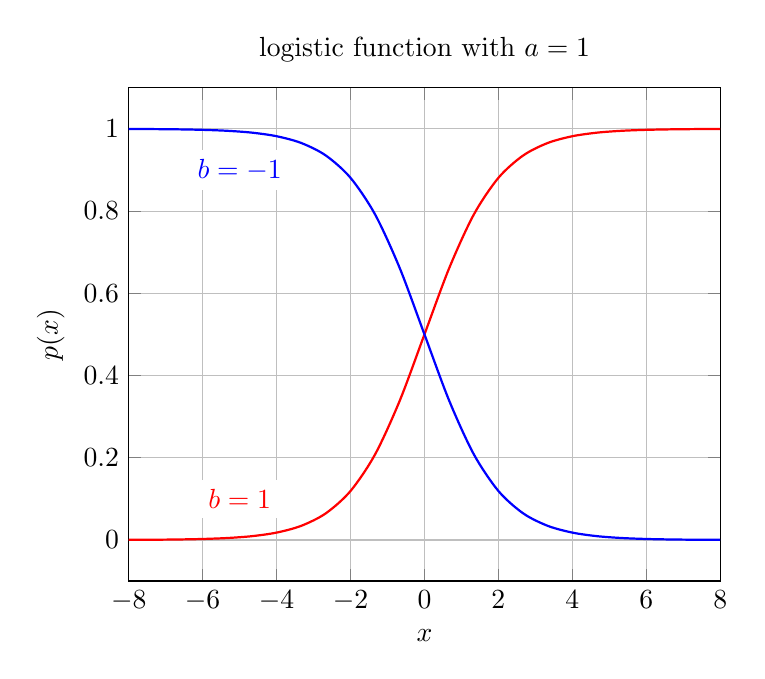
\begin{tikzpicture}
		\begin{axis}[width = 0.75\textwidth,xlabel=$x$, ylabel=$ p(x) $, grid = both, xmin = -8, xmax = 8, title = {logistic function with $ a = 1 $}]
			\addplot[thick, smooth, draw=red][name path = f1, domain = -8:8]{exp(x)/(1 + exp(x))};
			\addplot[thick, smooth, draw=blue][name path = f2, domain = -8:8]{exp(-x)/(1 + exp(-x))};
			
			
			\node[color=red, fill=white] at (axis cs: -5,.1) {$ b = 1 $};
			\node[color=blue, fill=white] at (axis cs: -5,.9) {$ b = -1 $};
			
			
		\end{axis}
	\end{tikzpicture}
\end{figure}


In order to find the maximum likelihood estimators, consider the joint PDF of a set of binary responses $ \{Y_1, \dots, Y_k\} $,

\begin{align}
	\log(P\{Y_i = y_i;\ i = 1,\dots,k\}) &= \sum\limits_{i = 1}^{k} y_i (a + bx_i) - \sum\limits_{i = 1}^{k} \log(1 + \exp(a +b x_i))
\end{align}

Even though an analytical minimization of the above expression is not possible, there are several iterative computational approaches possible.



\chapter{Analysis of Variance}


\begin{flushright}
	\textit{``What do you mean `Its a method used to compare mean values'?"} 
\end{flushright}

\section{Introduction}

Consider the problem of testing whether alternative approaches to solving a problem are equivalent. A simple null hypothesis is to ask if the average benefit of each problem-solving approach is the same.
	
A standard procedure to test this would be to randomly divide a population into many subgroups, each subjected to a different solution. The null hypothesis, under the assumption that the response of each individual tested has a variance independent of the solution itself, is simply the subgroup-means being equal.

\section{Overview of the procedure}

Consider a set of $ m $ populations from which samples of size $ n $ are drawn. Proving the equality of the means of these populations, which only depend on one parameter, namely the population the sample was from, is called a \textit{one-way} analysis of variance.

This can also be extended to the more general case of the $ m $ different samples not being of equal size.

The more complex case of the variance of each variable depending on two factors, the population index as well as the sample index, can be visually represented as a two-dimensional array with row and column indices both determining the variance. This is called the \textit{two-way} analysis of variance problem.

The above problem assumes no interaction between the two factors affecting the mean of the variable. Removing this assumption makes for a significantly more complicated problem, with possible non-linear interactions among the factors affecting the mean.

For the rest of this chapter, a general procedure can be outlined as follows,

\begin{itemize}
	\item Assume samples are drawn from a normal population with unknown (but common) variance $ \sigma^2 $
	\item Find a valid estimator of $ \sigma^2 $, which is true regardless of the specific null hypothesis being true.
	\item Fina another estimator of $ \sigma^2 $ which is true only when $ H_0 $ holds.
	\item Design a test that rejects $ H_0 $ when the second estimator is sufficiently larger than the first (since it tends to always be larger). 
\end{itemize}


Consider a set of $ N $ independent normal RVs $ \{X_i\} $ with possibly different means but a common unknown variance. 

\begin{align}
	\frac{X_i - \mu_i}{\sigma} &\sim Z_i \nonumber \\
	%
	\sum\limits_{i = 1}^{N} \frac{(X_i - \mu_i)^2}{\sigma^2} &\sim \chi^2_{N} \nonumber \\
\end{align}

If each $ \mu_i  = \mathbb{E}[X_i]$ can be estimated using a linear combination of $ k $ parameters, then the resulting estimate of the means $ \{\widehat{\mu_i}\} $, can be substituted into the above expression to make a $ \chi^2 $ distribution with $ (N-k) $ DOF.

\section{One-way ANOVA}

Consider a set of $ m $ samples, each of size $ n $ (\textit{balanced samples}). The members of each sample are independent normal RVs and a hypothesis testing the equality of their means,

\begin{align}
	X_{ij} &\sim \mathcal{N}(\mu_i, \sigma^2) \qquad i = 1,\dots,m \qquad j = 1,\dots,n \\
	%
	H_0 &: \mu_1 = \mu_2 = \dots = \mu_m \qquad \text{vs} \qquad H_1 : \text{not all means are equal}
\end{align}

Using the set of sample means $ \{X_{i\bullet}\} $ of the $ n $ populations as the estimators for $ \{\mu_i\} $,

\begin{align}
	\sum\limits_{i = 1}^{m} \sum\limits_{j = 1}^{n} \frac{(X_{ij} - \mathbb{E}[X_{ij}])^2}{\sigma^2} &\sim \chi^2_{nm} \\
	%
	\sum\limits_{i = 1}^{m} \sum\limits_{j = 1}^{n} \frac{(X_{ij} - X_{i\bullet})^2}{\sigma^2} &\sim \chi^2_{nm - m} 
\end{align}

Defining the \textit{within-samples sum of squares} ($ SS_W $) as 

\begin{align}
	SS_W &= \sum_{i} \sum_{j} (X_{ij} - X_{i\bullet})^2 \\
	%
	\sum_{i} \sum_{j} \frac{SS_W}{\sigma^2} &\sim \chi^2_{nm-m} \\
	%
	\mathbb{E}\left[\frac{SS_W}{\sigma^2}\right] &= nm - m \\
	%
	\sigma^2 &= \frac{SS_W}{nm-m}
\end{align}

The above estimator of $ \sigma^2 $ is free of any assumptions about the $ H_0 $. Next, under the assumption that $ H_0 $ holds, and thus the set of population means $ \{X_{i\bullet}\} $ are all normal RVs with common mean $ \mu $ and common variance $ \sigma^2 / n $,

\begin{align}
	n\ \sum\limits_{i = 1}^{m} \frac{(X_{i\bullet} - \mu)^2}{\sigma^2} &\sim \chi^2_{m} \\
	%
	X_{\bullet \bullet} &= \frac{\sum_{i} \sum_{j} X_{ij}}{nm} = \frac{\sum_{i} X_{i\bullet}}{m} \\
\end{align}

Since the above mean of all variables $ X_{\bullet \bullet} $ is an estimator of the common mean $ \mu $ which requires only $ 1 $ parameter to calculate, the \textit{between-samples sum of squares} ($ SS_b $) can be used to simplify the above expression,

\begin{align}
	SS_b &= n\ \sum\limits_{i = 1}^{m} (X_{i\bullet} - X_{\bullet\bullet})^2 \\
	%
	\frac{SS_b}{\sigma^2} &\sim \chi^2_{m-1} \nonumber \\
	%
	\frac{SS_b}{(m-1)} &= \sigma^2
\end{align}

Since the conditional estimator of $ \sigma^2 $ tends to be larger and these two estimators are independent when $ H_0 $ holds, the ratio of these two $ \chi^2 $ RVs to define an f-RV, the hypothesis test can be formulated as,

\begin{align}
	\frac{SS_b}{SS_W}\ \frac{(nm-m)}{(m-1)} &\sim F_{m-1, nm-m} \nonumber \\
	%
	H_0 : \text{all means are equal} \qquad &\text{vs.} \qquad H_1 : \text{not all means are equal} \nonumber \\
	%
	\text{reject $ H_0 $ if } \qquad & \frac{SS_b}{SS_W}\ \frac{(nm-m)}{(m-1)} > F_{\alpha, m-1, nm-m}  \nonumber \\
	%
	\text{accept $ H_0 $} \qquad & \text{otherwise}
\end{align}

A computational identity relating the two terms $ SS_b $ and $ SS_W $ is as follows,

\begin{align}
	\sum\limits_{i = 1}^{m} \sum\limits_{j = 1}^{n} X^2_{ij} &= nm\ X^2_{\bullet \bullet} + SS_b + SS_W
\end{align}

A proof of the relation between the two estimates of $ \sigma^2 $, uses the following variable transformation,

\begin{align}
	\mathbb{E}\left[\frac{SS_b}{(m-1)}\right] &\geq \sigma^2 \qquad \text{equality only if $H_0$ holds} \\
	%
	Y_i &= X_{i\bullet} -\mu_i + \mu_{\bullet} \nonumber \\
	%
	\mathbb{E}\left[\frac{\sum_{i} (X_{i\bullet} - X_{\bullet\bullet})^2}{(m-1)}\right] &= \frac{\sigma^2}{n} + \sum_{i} \frac{(\mu_i - \mu_{\bullet})^2}{(m-1)}
\end{align}

\textit{Multiple comparisons of sample means} : When the null hypothesis above is rejected, a measure of how the different sample means are related is the T-method. This gives a confidence interval for the difference between all possible pairs $ \mu_i - \mu_j $. 

\begin{align}
	\mu_i - \mu_j &\in X_{i\bullet} - X_{j\bullet} \pm W \\
	%
	\forall \ i\neq j &\qquad \text{with probability $ 1-\alpha $} \nonumber \\
	%
	W &= \frac{1}{\sqrt{n}} \ q(m, nm-m, \alpha)\ \sqrt{\frac{SS_W}{(nm-m)}}
\end{align}

Here, the studentized range distribution $ q $ has pre-calculated CDF tables. Further information in article - \textit{Tukey's range test}.

\textit{Unequal sample sizes (unbalanced)} : Since the assumption of sample sizes all being equal to $ n $ is no longer valid, it is replaced with sample sizes $ \{n_1, n_2, \dots, n_m\} $ for each of the $ m $ samples.

For convenience, define $ N = \sum_i n_i $.

\begin{align}
	\sum\limits_{i = 1}^{m} \sum\limits_{j = 1}^{n_i} \frac{(X_{ij} - \mu_i)^2}{\sigma^2} &\sim \chi^2_{N} \\
	%
	\sum\limits_{i = 1}^{m} \sum\limits_{j = 1}^{n_i} \frac{(X_{ij} - X_{i\bullet})^2}{\sigma^2} &\sim \chi^2_{N - m} \\
\end{align}

Once again, defining $ SS_W $ and simplifying yields an unbiased estimator of $ \sigma^2 $ not dependent on $ H_0 $.

\begin{align}
	SS_W &= \sum\limits_{i = 1}^{m} \sum\limits_{j = 1}^{n_i} (X_{ij} - X_{i\bullet})^2 \\
	%
	\frac{SS_W}{N-m} &= \sigma^2
\end{align}

Next, under the assumption that $ H_0 $ holds, and the means are equal to a common value $ \mu $.

\begin{align}
	\mathbb{E}[X_{i\bullet}] &= \mu & \mathrm{Var}(X_{i\bullet}) &= \frac{\sigma^2}{n_i} \nonumber \\
	%
	\sum\limits_{i = 1}^{m} \frac{(X_{i\bullet} - \mu)^2}{\sigma^2 / n_i} &\sim \chi^2_{m} & \sum\limits_{i = 1}^{m} \frac{(X_{i\bullet} - X_{\bullet\bullet})^2}{\sigma^2 / n_i} &\sim \chi^2_{m-1} \\
	%
	SS_b &= \sum\limits_{i = 1}^{m} n_i\ (X_{i\bullet} - X_{\bullet\bullet})^2
\end{align}

When $ H_0 $ is true, both the estimators of $ \sigma^2 $ are unbiased and independent. This enables the construction of a level $ \alpha $ hypothesis test

\begin{align}
	\frac{SS_b}{SS_W}\ \frac{(N-m)}{(m-1)} &\sim F_{m-1, N-m} \nonumber \\
	%
	H_0 : \text{all means are equal} \qquad &\text{vs.} \qquad H_1 : \text{not all means are equal} \nonumber \\
	%
	\text{reject $ H_0 $ if } \qquad & \frac{SS_b}{SS_W}\ \frac{(N-m)}{(m-1)} > F_{\alpha, m-1, N-m}  \nonumber \\
	%
	\text{accept $ H_0 $} \qquad & \text{otherwise}
\end{align}

Balanced samples are more robust to violations of the assumption of equal variances of the different populations and thus preferred over unbalanced samples.

\section{Two-factor ANOVA}

Consider the more complex where each data value in the data-set is affected by two factors, with ($ m, n $) \textit{levels} respectively. The dataset can be arranged into a two-dimensional array along these two indices.

\begin{align}
	\begin{bmatrix}
		X_{11} & X_{12} & X_{13} & \dots & X_{1n} \\
		X_{21} & X_{22} & X_{23} & \dots & X_{2n} \\
		\vdots & \vdots & \vdots & \ddots & \vdots \\
		X_{i1} & X_{i2} & X_{i3} & \dots & X_{in} \\
		\vdots & \vdots & \vdots & \ddots & \vdots \\
		X_{m1} & X_{m2} & X_{m3} & \dots & X_{mn} \\
	\end{bmatrix}
\end{align}

By convention the factors are called the \textit{row-factor} and \textit{column-factor} respectively. The mean value of a data point depends additively on both its row and column index.

Let $ \mu_{ij} = \mathbb{E}[X_{ij}] $, where $ i \in \{1, \dots, m\} $ and $ j \in \{1, \dots, n\} $.

\begin{align}
	\mu_{ij} &= a_i + b_j & \mu = \mu_{\bullet\bullet} &= \sum\limits_{i = 1}^{m} \sum\limits_{j = 1}^{n} \frac{\mu_{ij}}{nm} \\
	%
	\mu_{\bullet j} &= a_{\bullet} + b_j & \mu_{i \bullet} &= a_{i} + b_{\bullet} \\
	%
	\alpha_i &= a_i - a_{\bullet} & \beta_j &= b_j - b_{\bullet}
\end{align}

The \textit{grand mean} is defined as the mean of all terms $ \mu \coloneqq \mu_{\bullet \bullet} $, and the terms $ \alpha_i, \beta_j $ are the row and column \textit{deviations} from the grand mean.

The model can now be rewritten as

\begin{align}
	\mu_{ij} = \mathbb{E}[X_{ij}] &= \mu + \alpha_i + \beta_j \\
	%
	\sum_{i} \alpha_i &= \sum_{j} \beta_j = 0 
\end{align}

Using the row-average, column-average and overall-average of the data points, $ X_{i\bullet},\ X_{\bullet j},\ X_{\bullet \bullet} $ to calculate the estimators of $ \alpha_i, \beta_j, \mu $ respectively,

\begin{align}
	\mathbb{E}[X_{i\bullet}] &= \mu + \alpha_i & \mathbb{E}[X_{\bullet j}] &= \mu + \beta_j \\
	%
	\mathbb{E}[X_{i\bullet} - X_{\bullet \bullet}] &= \alpha_i & \mathbb{E}[X_{\bullet j} - X_{\bullet \bullet}] &=  \beta_j 
\end{align}

This leads to the following unbiased estimators of the model parameters.

\begin{align}
	\widehat{\mu} &= X_{\bullet \bullet} \nonumber \\
	%
	\widehat{\alpha_i} &= X_{i\bullet} - X_{\bullet \bullet} \nonumber \\
	%
	\widehat{\beta_j} &= X_{\bullet j} - X_{\bullet \bullet}
\end{align}

\section{Two-factor ANOVA : Hypothesis testing} 

The most common hypothesis to be tested is the absence of any effect due to the row-factors or the column-factors.

\begin{align}
	H_0 : \text{all $ \alpha_i $ are zero} \qquad \text{vs} \qquad H_1 : \text{not all $ \alpha_i $ are zero} \nonumber \\
	H_0 : \text{all $ \beta_j $ are zero} \qquad \text{vs} \qquad H_1 : \text{not all $ \beta_j $ are zero} \nonumber
\end{align}

Using the usual ANOVA procedure of comparing two different estimators of the variance,

\begin{align}
	\sum\limits_{i = 1}^{m} \sum\limits_{j = 1}^{n} \frac{(X_{ij} - \mathbb{E}[X_{ij}])^2}{\sigma^2} &\sim \chi^2_{mn} \nonumber \\
	%
	\sum\limits_{i = 1}^{m} \sum\limits_{j = 1}^{n} \frac{(X_{ij} - \widehat{\mu} - \widehat{\alpha_i} - \widehat{\beta_j})^2}{\sigma^2} &= \sum\limits_{i = 1}^{m} \sum\limits_{j = 1}^{n} \frac{(X_{ij} + X_{\bullet \bullet} - X_{i \bullet} - X_{\bullet j})^2}{\sigma^2}
\end{align}

The number of parameters required to estimate the above 3 parameters is $ 1 + (m-1) + (n-1) = (m+n-1)$. This leaves a $ \chi^2 $ RV with $ mn - (m+n-1) = (m-1)(n-1) $ DOF. Using the definiton of the \textit{error sum of squares},

\begin{align}
	SS_e &=	\sum\limits_{i = 1}^{m} \sum\limits_{j = 1}^{n} (X_{ij} - X_{\bullet \bullet} - X_{i \bullet} - X_{\bullet j})^2\\
	%
	\frac{SS_e}{(m-1)(n-1)} &= \sigma^2
\end{align}

To find the $ H_0 $ conditioned estimator of $ \sigma^2 $, first consider the case where all of the row-factors are zero.

\begin{align}
	\mathbb{E}[X_{i\bullet}] &= \mu + \alpha_i = \mu & \mathrm{Var}(X_{i\bullet}) &= \frac{\sigma^2}{n} \nonumber \\
	%
	\text{if $ H_0 $ is true, } && n\sum\limits_{i = 1}^{m} \frac{(X_{i\bullet}  - \mu)^2}{\sigma^2} &\sim \chi^2_{m} \\
	%
	n\sum\limits_{i = 1}^{m} \frac{(X_{i\bullet}  - X_{\bullet \bullet})^2}{\sigma^2} &\sim \chi^2_{m-1}
\end{align}

Defining the \textit{row sum of squares} and analogously the \textit{column sum of squares},

\begin{align}
	SS_r &= n\sum\limits_{i = 1}^{m} (X_{i\bullet}  - X_{\bullet \bullet})^2 & SS_c &= m\sum\limits_{j = 1}^{n} (X_{\bullet i}  - X_{\bullet \bullet})^2 
\end{align}

Using the above definitions, a second estimator for $ \sigma^2 $ conditioned on $ H_0 $ being true is,

\begin{align}
	\frac{SS_r}{(m-1)} &= \sigma^2 & \frac{SS_r}{SS_e}\ \frac{(m-1)(n-1)}{(m-1)} &\sim F_{m-1, (m-1) (n-1)}
\end{align}

The hypothesis test can now be constructed using this F-RV as follows,

\begin{align}
	H_0 : \text{all row-factors are zero} \qquad &\text{vs.} \qquad H_1 : \text{not all row-factors are zero} \nonumber \\
	%
	\text{reject $ H_0 $ if } \qquad & \frac{SS_r}{SS_e}\ \frac{(m-1)(n-1)}{(m-1)} > F_{\alpha, m-1, (m-1) (n-1)} \nonumber \\
	%
	\text{accept $ H_0 $} \qquad & \text{otherwise}
\end{align}

\section{Two-way ANOVA with interaction} 

Extending the model in the previous section to allow the possibility of some interaction between the row and column factors governing a particular data-point,

\begin{align}
	\mu_{ij} &= \mathbb{E}[X_{ij}] & \mu_{ij} &= \mu + \alpha_i + \beta_j + \gamma_{ij} \\
	%
	\mu &= \mu_{\bullet \bullet} & \gamma_{ij} &= \mu_{ij} - \mu_{i\bullet} - \mu_{\bullet j} + \mu_{\bullet \bullet} \\
	%
	\alpha_i &= \mu_{i\bullet} - \mu_{\bullet \bullet} & \beta_j &= \mu_{\bullet j} - \mu_{\bullet \bullet} \\
	%
	\sum\limits_{i = 1}^{m} \gamma_{ij} &= 0 & \sum\limits_{j = 1}^{n} \gamma_{ij} &= 0
\end{align}

In addition, the usual constraints on the set of $ \{\alpha_i\} $ and $ \{\beta_j\} $ summing to zero still apply. In this extended mode, the term $ \gamma_{ij} $ is called the \textit{interaction of row i and column j}. It measures the difference between the mean of $ X_{ij} $ and the three terms indicating the grand mean, row effect and column effect.

For mathematical reasons, it is no longer sufficient to have just one observation for a given row and column index. Assume there are a set of $ l $ such observations corresponding to every possible pair of $ \{i, j\} $. Since each data point $ X_{ijk} $ is still a normal RV with common unknown variance $ \sigma^2 $,

\begin{align}
	X_{ijk} &\sim \mathcal{N}(\mu + \alpha_i + \beta_j + \gamma_{ij},\ \sigma^2) & k &\in \{1, \dots, l\} \\
	%
	i &\in \{1, \dots, m\} & j &\in \{1, \dots n\} \nonumber 
\end{align}

To find the estimators for the three sets of parameters defined above, use,

\begin{align}
	\mathbb{E}[X_{ij\bullet}] &= \mu_{ij} & \mathbb{E}[X_{\bullet \bullet \bullet}] &= \mu \\
	%
	\mathbb{E}[X_{i\bullet \bullet}] &= \mu + \alpha_i & \mathbb{E}[X_{\bullet j \bullet}] &= \mu + \beta_j
\end{align}

Using the fact that substituting the parameters above with their unbiased estimators will lead to a reduction in DOF of the $ \chi^2 $ RV,

\begin{align}
	\widehat{\mu} &= X_{\bullet \bullet \bullet} \nonumber \\
	%
	\widehat{\alpha_i} &= X_{i\bullet \bullet} - X_{\bullet \bullet \bullet} \nonumber \\
	%
	\widehat{\beta_j} &= X_{\bullet j \bullet} - X_{\bullet \bullet \bullet} \nonumber \\
	%
	\widehat{\gamma_{ij}} &= X_{ij\bullet} - X_{i\bullet \bullet} - X_{\bullet j \bullet} + X_{\bullet \bullet \bullet} 
\end{align}

For hypothesis tests asking whether one of the three sets of parameters are all zeros, arrange $ \chi^2 $RVs as follows,

\begin{align}
	\sum\limits_{i = 1}^{m} \sum\limits_{j = 1}^{n} \sum\limits_{k = 1}^{l}\frac{(X_{ijk} - \mathbb{E}[X_{ijk}])^2}{\sigma^2} &\sim \chi^2_{mnl} \nonumber \\
	%
	\sum\limits_{i = 1}^{m} \sum\limits_{j = 1}^{n} \sum\limits_{k = 1}^{l} \frac{(X_{ij} - \widehat{\mu} - \widehat{\alpha_i} - \widehat{\beta_j} - \widehat{\gamma_{ij}})^2}{\sigma^2} &\sim \chi^2_{mnl - mn}
\end{align}

The number of parameters needed to estimate $ \widehat{\mu},\ \widehat{\alpha_i},\ \widehat{\beta_j},\  \widehat{\gamma_{ij}} $ are $ 1,\ (m-1),\ (n-1),\ (m-1)(n-1) $ respectively. This means that the loss in DOF is $ mn $.

Now, defining the \textit{error sum of squares} $ SS_e $ as

\begin{align}
	SS_e &= \sum\limits_{i = 1}^{m} \sum\limits_{j = 1}^{n} \sum\limits_{k = 1}^{l} (X_{ijk} - X_{ij\bullet})^2 \\
	%
	\frac{SS_e}{(mnl  - mn)} &= \sigma^2
\end{align}

Having found the true estimator of the variance, now consider the estimator conditioned on the null hypothesis that there are no interaction terms. Now, each of the variables $ X_{ij\bullet} $ is averaged over $ l $ data points, and thus

\begin{align}
	H_0^{\textit{int}} : \gamma_{ij} &= 0 & \forall\ &i,j \nonumber \\
	%
	\mathbb{E}[X_{ij\bullet}] &= \mu + \alpha_i + \beta_j & \mathrm{Var}(X_{ij\bullet}) &= \frac{\sigma^2}{l} \\
	%
	\sum\limits_{i = 1}^{m} \sum\limits_{j = 1}^{n} \frac{(X_{ij\bullet} - \mu - \alpha_i - \beta_j)^2}{\sigma^2 / l} &\sim \chi^2_{mn}
\end{align}

From an earlier section, replacing the parameters above with their estimators involes an $ m+n-1 $ loss in DOF. Defining the \textit{non-interaction sum of squares} ($ SS_{int} $) \\

\begin{align}
	SS_{int} &= \sum\limits_{i = 1}^{m} \sum\limits_{j = 1}^{n}\ l\ (X_{ij\bullet} - X_{i\bullet \bullet} - X_{\bullet j \bullet} + X_{\bullet \bullet \bullet})^2 \\
	%
	\frac{SS_{int}}{(n-1)(m-1)} &= \sigma^2 \qquad \text{if $ H_0^{int} $ holds}
\end{align}

Using the two estimators of $ \sigma^2 $ above, an F-RV can be created to test the null hypothesis at significance level $ a $ as follows,

\begin{align}
	H_0^{int} : \text{all $ \gamma{ij} $ are zero} \qquad &\text{vs.} \qquad H_1^{int} \nonumber \\
	%
	\text{reject $ H_0 $ if } \qquad & \frac{SS_{int}}{SS_e}\ \frac{(mnl - mn)}{(n-1)(m-1)} > F_{a,(m-1)(n-1), mnl-mn} \nonumber \\
	%
	\text{accept $ H_0 $} \qquad & \text{otherwise}
\end{align}

Similar hypothesis tests for row-factors or column-factors being all zero, involve the \textit{row sum of squares} and \textit{column sum of squares} respectively. For example the null hypothesis $ H_0^r : \text{all $ \alpha_i $ are zero} $ can be tested using

\begin{align}
	SS_r &= \sum\limits_{i = 1}^{m} \ nl\ (X_{i\bullet \bullet} - X_{\bullet \bullet \bullet})^2 \\
	%
	\frac{SS_{r}}{SS_e}\ \frac{(mnl - mn)}{(m-1)} &\sim F_{m-1, mnl-mn} 
\end{align}

An analogous expression can be written for the null hypothesis $ H_0^c : \text{all $ \beta_j $ are zero} $.

Note that the procedure in the later sections is a straightforward increase in complexity from the same procedure in earlier sections which was outlined in the introduction as the general ANOVA approach.
\chapter{Goodness of Fit Tests and Categorical Data Analysis}


\begin{flushright}
	\textit{``You are going to have to refer to published p-value tables for this test unfortunately."}
\end{flushright}

\section{Introduction}

The \textit{a priori} assumption of a probability model governing an observed phenomenon is central to the analysis of samples from an underlying population. The measure appropriateness for this assumed probability model is done through \textit{goodness-of-fit} tests.

The null hypothesis to be tested is that a sample has the specified probability distribution. The parameters of this probability distribution may not be fully specified, leading to a more complex problem.

\section{Goodness of fit tests with all parameters specified}

Consider a set of $ n $ independent random variables $ \{Y_j\} $ each of which can take on discrete values in the integer set $ \{1, \dots , k\} $. The null hypothesis to test is that they all have the same underlying PMF, specified as

\begin{align}
	H_0 &: P\{Y = i\} = p_i \qquad \forall \ i \in \{1, \dots , k\} \\
	%
	H_1 &: P\{Y = i\} \neq p_i \qquad \text{for some}\  i \in \{1, \dots , k\} \nonumber
\end{align}

Defining the set $ \{X_i\} $ as the number of RVs $ \{Y_j\} $ which have the value $ i $, it follows that the set $ \{X_i\} $ are independent binomial RVs with parameters $ \{(n, p_i)\} $ under $ H_0 $\\

\begin{align}
	X_i &\sim \texttt{Binom} (n,\ p_i) \\
	%
	\mathbb{E}[X_i] &= np_i
\end{align}

A method of judging how close $ p_i $ is to the actual probability $ P\{Y = i\} $, is to look at a standardized sum of squared errors, and use it to define a test statistic.

Using a significance threshold $ \alpha $, and the fact that $ T $ approaches a $ \chi^2 $ RV with $ (k-1) $ DOF as $ n \to \infty $,


\begin{align}
	T &= \sum\limits_{i=1}^{k} \frac{(X_i - np_i)^2}{np_i}  \\
	%
	\lim\limits_{n \to \infty} T &\to \chi^2_{k-1} \\[1ex]
	%
	\text{reject $ H_0 $ if } \qquad & T > \chi^2_{\alpha, k-1}  \nonumber \\
	%
	\text{accept $ H_0 $} \qquad & \text{otherwise}
\end{align}

A rule of thumb for sample sizes in the test above is to ensure that in the set $ \{np_i\} $, all values exceed 1 and most exceed 5.

A simpler expression for $ T $ exploits the fact that $ \sum X_i = n $ and $ \sum p_i = 1 $. This constraint on the $ {X_i} $ is also responsible for the $ \chi^2 $ RV having $ (k-1) $ DOF.

\begin{align}
	T = \sum\limits_{i=1}^{k} \frac{(X_i - np_i)^2}{np_i} = \sum\limits_{i=1}^{k} \frac{X_i^2}{np_i}\ -\ n
\end{align}

\textit{Simulation-based methods of determining critical region} : Until the modern computer age led to computing power being cheap and widely available, the above $ \chi^2 $ approximation was the only method of defining critical regions for the goodness-of-fit test.

Consider a set of randomly generated variables $ \{Y_1^{(1)}, \dots, Y_n^{(1)}\} $, each having the PMF $ P\{Y_j^{(1)} = i\} = p_i $ for $ i \in \{1, \dots, k\} $.

Defining the set $ \{X_i^{(1)}\} $ and test statistic $ T^{(1)} $ as above,

\begin{align}
	X_i^{(1)} &= \text{number of} \ j : Y_j^{(1)} = i \\
	%
	T^{(1)} &= \sum\limits_{i=1}^{k} \frac{(X_i^{(1)} - np_i)^2}{np_i}
\end{align}

Using the above procedure to generate a large number of test statistics $ \{T^{(1)}, \dots, T^{(r)}\} $ by repetition of the above procedure yields an approximation to the probability distribution of $ T $.

\begin{align}
	P_{H_0} (T \geq t) &\approxeq \frac{\text{number of}\ l : T^{(l)} \geq t}{r}
\end{align}

The above approximation becomes very accurate for large $ r $ and can also be used then to calculate a p-value for the test. The generation of a random set $ \{Y^{(r)}\} $ exploits the Monte-Carlo system of using a standard uniform RV transformed using the set of probabilities $ \{p_i\} $ to output the discrete value of $ Y^{(r)}_j $.

\section{Goodness of fit tests with some parameters unspecified}

When the underlying probability distribution is not fully specified, a general strategy is to divide the possible continuous set of outcomes into a few discrete regions. Using the observed set of data points to calculate an estimate for the unspecified parameters, an estimated test statistic can then be calculated.

\begin{align}
	P\{Y_j = i\} &= p_i \qquad \text{where} \qquad \widehat{p_i} \approx p_i \\
	%
	T &= \sum\limits_{i=1}^{k} \frac{(X_i - n\widehat{p_i})^2}{n\widehat{p_i}} \\
	%
	\lim\limits_{n \to \infty} & T \to \chi^2_{k-1-m} \\[1ex]
	%
	\text{reject $ H_0 $ if } \qquad & T > \chi^2_{\alpha, k-1-m}  \nonumber \\
	%
	\text{accept $ H_0 $} \qquad & \text{otherwise}
\end{align}

In the calculation of $ \widehat{p_i} $ above, the CDF of the underlying probability distribution assumed by $ H_0 $, with estimated parameters $ \{\widehat{\lambda}\} $ is used along with the user-defined discrete outcomes. The $ \chi^2 $ RV has $ (k-1-m) $ DOF if there are $ m $ unspecified parameters to be estimated.

For example, a set of observed data with a null hypothesis of the underlying distribution being Poisson, would involve estimating the unspecified mean of the Poisson distribution $ \widehat{\lambda} $ using the observations and then calculating the test statistic and p-value.

\section{Tests of independence in contingency tables}

Consider a population whose members are governed by two characteristics ($ X, Y $) each of which can take $ (r, s) $ possible values. The marginal probabilities can then be calculated as,

\begin{align}
	P_{ij} &= P\{X = i, Y = j\} \qquad i \in \{1, \dots, r\} \qquad j \in \{1, \dots, s\} \\[1ex]
	%
	p_i &= P\{X = i\} = \sum_j\ P_{ij} \qquad i \in \{1, \dots, r\} \\
	%
	q_j &= P\{Y = j\} = \sum_i\ P_{ij} \qquad j \in \{1, \dots, s\}
\end{align}

The null hypothesis of interest here is to test the independence of the $ X $ and $ Y $ characteristics.

\begin{align}
	H_0 &: P_{ij} = p_i q_j \qquad \forall \ \text{possible pairs $ (i, j) $}\\
	%
	H_1 &: P_{ij} \neq p_i q_j \qquad \text{for some pair $ (i, j) $}
\end{align}

Let the set of $ n $ observations be arranged into a  \textit{contingency table} where each element $ N_{ij} $ represents the number of observations with $ X=i, Y=j $. The marginal probabilities can be estimated from the data set as

\begin{align}
	N_i &= \sum_j N_{ij} & \widehat{p_i} &= \frac{N_i}{n} \\
	%
	M_j &= \sum_i N_{ij} & \widehat{q_j} &= \frac{M_j}{n}
\end{align}

When $ H_0 $ is true, a test statistic can be set up as,

\begin{align}
	\mathbb{E}[N_{ij}] &= nP_{ij} = p_i q_j \qquad \text{assuming $ H_0 $ true} \\
	%
	T &= \sum\limits_{i=1}^{r} \sum\limits_{j=1}^{s} \ddfrac{(N_{ij} - n\widehat{p}_i \widehat{q}_j)^2}{n\widehat{p}_i \widehat{q}_j} \nonumber \\
	%
	&= \sum\limits_{i=1}^{r} \sum\limits_{j=1}^{s} \ddfrac{N_{ij}^2}{n\widehat{p}_i \widehat{q}_j}\ -\ n
\end{align}

The reduction in DOF is $ (1 + (r-1) + (s-1)) $. This leads to $ T \sim \chi^2_{(r-1)(s-1)} $ since there are a total of $ r \times s $ possible categories into which each observation can belong.

\begin{align}
	\lim\limits_{n \to \infty} & T \to \chi^2_{(r-1)(s-1)} \\[1ex]
	%
	\text{reject $ H_0 $ if } \qquad & T > \chi^2_{\alpha, (r-1)(s-1)}  \nonumber \\
	%
	\text{accept $ H_0 $} \qquad & \text{otherwise}
\end{align}

\section{Tests of independence in contingency tables with fixed marginal totals}

If the sample is chosen such that the row sum and/or column sum is fixed across all rows and/or columns, the procedure used in the above section is largely unchanged. Defining the sample incidence of each pair of characteristics $ \widehat{e}_{ij} $, and then a test statistic,

\begin{align}
	\widehat{e}_{ij} &= n\widehat{p}_i \widehat{q}_j = \frac{N_i M_j}{n} \\
	%
	T &= \sum_{i} \sum_{j} \frac{(N_{ij} - \widehat{e}_{ij})^2}{\widehat{e}_{ij}}
\end{align}

Here, $ N_i $ and $ M_j $ are the row-sums and column-sums respectively. The rest of the test is also unchanged with the use of a $ \chi^2 $ RV with $ (r-1)(s-1) $ DOF used to calculate the critical regions.


An extension of the above procedure can be used to test the hypothesis that $ m $ populations with each member taking on one of $ n $ possible values, all have the same discrete population distribution.

\begin{table}[H]
	\renewcommand{\arraystretch}{2}
	\centering
	\begin{tabular}{@{}rrrrrr|l@{}}
		\toprule
		Value 	& \multicolumn{5}{c}{Population}	& Row Sum\\ 
		\midrule
		{} & $ 1 $	& $ 2 $	& \dots & $ j $ & $ n $ & {} \\
		\midrule
		$ 1 $ & $ N_{11} $ & $ N_{12} $ & \dots &  $ N_{1j} $ & $ N_{1n} $ & $ M_{1} $ \\
		$ 2 $ & $ N_{21} $ & $ N_{22} $ & \dots &  $ N_{2j} $ & $ N_{2n} $ & $ M_{2} $ \\
		$ \vdots $ & $ \vdots $ & $ \vdots $ & $ \ddots $ &  $ \vdots $ & $ \vdots $ & $ \vdots $ \\
		$ i $ & $ N_{i1} $ & $ N_{i2} $ & \dots &  $ N_{ij} $ & $ N_{in} $ & $ M_{i} $ \\
		$ m $ & $ N_{m1} $ & $ N_{m2} $ & \dots &  $ N_{mj} $ & $ N_{mn} $ & $ M_{m} $ \\
		\midrule
		Column Sum & $ N_1 $ & $ N_2 $ & \dots &  $ N_j $ & $ N_n $ & {} \\ 
		\bottomrule
	\end{tabular}
	
	\bigskip
\end{table}

The hypothesis above now reduces to the absence of a row effect in the table of observations. $ H_0 : p_{1j}  = p_{2j} = \dots  = p_{mj}$\\

\section{Kolmogorov-Smirnov goodness of fit test for continuous data}

Given a set of samples $ \{Y_i\} $ from an underlying population distribution, the hypothesis testing whether this distribution is some continuous CDF given by $ F $ can be performed using the discretization procedure from the previous section.

Let the range $ (-\infty, \infty) $ be broken up into $ k $ parts. Now, the observations can belong to one of these $ k $ categories as

\begin{align}
	Y^d_j &= i & \text{if}\ Y_j &\in (y_{i-1}, y_i) \\
	%
	P\{Y_j^d = i\} &= F(y_i) - F(y_{i-1}) & \forall \ i &\in \{1,\dots,k\}
\end{align}

This creates a model that is amenable to the $ \chi^2 $ goodness-of-fit test outlined in the above sections.

Consider the alternative approach which involves estimating the CDF as an empirical distribution function $ F_e $,

\begin{align}
	F_e(x) &= \frac{\text{number of}\ i : Y_i \leq x}{n}
\end{align}

Here, $ F_e (x) $ is the proportion of observations that are less than or equal to $ x $. Since $ F_e (x) $ is an estimator of $ F(x) $ when $ H_0 $ is true, the \textit{Kolmogorov-Smirnov} test statistic is

\begin{align}
	D \equiv \max_{x}\  \Big|F_e (x) - F(x)\Big|
\end{align}

$ F_e (x) $ is a step-like function with step size $ 1/n $ and jumps at each of the data points $ \{Y_j\} $ after they have been rearranged into ascending order as $ \{Y_{(j)}\} $.

\begin{align}
	F_e (x) = 
	\begin{cases}
		0 & \text{if}\ x \in (-\infty,\ Y_{(1)}) \\
		%
		1/n & \text{if}\ x \in (Y_{(1)},\ Y_{(2)}) \\
		%
		\dots \\
		%
		(n-1) / n & \text{if}\ x \in (Y_{(n-1)},\ Y_{(n)}) \\
		%
		1 & \text{if}\ x \in (Y_{(n)},\ \infty) \\
	\end{cases}
\end{align}

Since $ F(x) $ itself is a monotonically increasing function, the expression $ |F_e (x) - F(x)| $ must have its maximum close to one of the points $ x = \{Y_{(j)}\} $. 

\begin{align}
	D = \max_j \left\{ \frac{j}{n} - F(y_{(j)}),\ F(y_{(j)}) - \frac{j-1}{n} \right\}
\end{align}

A p-value defined using this statistic does not depend on the choice of underlying distribution $ F $,

\begin{align}
	p = P_F (D \geq d) &= P_F \left\{ \max_x \Bigg| \frac{\#i : Y_i \leq x}{n}  - F(x)\Bigg| \geq d \right\}\\
	%	
	&= P \left\{ \max_x \Bigg| \frac{\#i : U_i \leq F(x)}{n}  - F(x)\Bigg| \geq d \right\}
\end{align}

The above uses the fact that if $ Y $ has a continuous CDF $ F $, then $ F(Y) $ is a standard uniform RV. This enables the use of independent standard uniform RVs $ \{U_i\} $ to ease the Monte-Carlo simulation of the p-value.

The Monte-Carlo procedure involves defning $ y = F(x) $ for the hypothesized CDF $ F $ and then performing many repeats of checking whether the following inequality holds,

\begin{align}
	\text{MC iteration } & \text{is}\ \max_{0 \leq y \leq 1} \Bigg| \frac{\#i : U_i \leq y}{n}  - y\Bigg| \geq d \\
	%
	\max_{y} \Bigg| \frac{\#i : U_i \leq y}{n}  - y\Bigg| &= \max_{j} \Bigg| \frac{j}{n} - U_{(j)},\ U_{(j)} - \frac{j-1}{n} \Bigg|
\end{align}


% bibliography, glossary and index would go here.

\end{document}